% -*- Mode:TeX -*-

%% IMPORTANT: The official thesis specifications are available at:
%%            http://libraries.mit.edu/archives/thesis-specs/
%%
%%            Please verify your thesis' formatting and copyright
%%            assignment before submission.  If you notice any
%%            discrepancies between these templates and the 
%%            MIT Libraries' specs, please let us know
%%            by e-mailing thesis@mit.edu

%% The documentclass options along with the pagestyle can be used to generate
%% a technical report, a draft copy, or a regular thesis.  You may need to
%% re-specify the pagestyle after you \include  cover.tex.  For more
%% information, see the first few lines of mitthesis.cls. 

%\documentclass[12pt,vi,twoside]{mitthesis}
%%
%%  If you want your thesis copyright to you instead of MIT, use the
%%  ``vi'' option, as above.
%%
%\documentclass[12pt,twoside,leftblank]{mitthesis}
%%
%% If you want blank pages before new chapters to be labelled ``This
%% Page Intentionally Left Blank'', use the ``leftblank'' option, as
%% above. 

\documentclass[12pt,twoside]{mitthesis}
\usepackage{lgrind}
\usepackage{graphicx}
\usepackage{amsmath}
\usepackage{booktabs}
\usepackage{float}
\usepackage{ amssymb }

\RequirePackage{doi}
\usepackage{hyperref}
\usepackage{url}
\usepackage{graphicx}
\usepackage[graphicx]{realboxes}
\usepackage{rotating}
\usepackage{CJKutf8}

\usepackage[labelformat=simple]{subcaption}
\renewcommand\thesubfigure{\alph{subfigure})}

\usepackage{comment}
\usepackage{natbib}
\setcitestyle{numbers}
\usepackage[compat=1.1.0]{tikz-feynman}

\usepackage{ifthen}
\pagestyle{plain}
\graphicspath{{figures/}}

\DeclareUnicodeCharacter{00A0}{ }
%% This bit allows you to either specify only the files which you wish to
%% process, or `all' to process all files which you \include.
%% Krishna Sethuraman (1990).
%
%\typein [\files]{Enter file names to process, (chap1,chap2 ...), or `all' to process all files:}
%\def\all{all}
%\ifx\files\all \typeout{Including all files.} \else \typeout{Including only \files.} \includeonly{\files} \fi

\begin{document}

% -*-latex-*-
% 
% For questions, comments, concerns or complaints:
% thesis@mit.edu
% 
%
% $Log: cover.tex,v $
% Revision 1.8  2008/05/13 15:02:15  jdreed
% Degree month is June, not May.  Added note about prevdegrees.
% Arthur Smith's title updated
%
% Revision 1.7  2001/02/08 18:53:16  boojum
% changed some \newpages to \cleardoublepages
%
% Revision 1.6  1999/10/21 14:49:31  boojum
% changed comment referring to documentstyle
%
% Revision 1.5  1999/10/21 14:39:04  boojum
% *** empty log message ***
%
% Revision 1.4  1997/04/18  17:54:10  othomas
% added page numbers on abstract and cover, and made 1 abstract
% page the default rather than 2.  (anne hunter tells me this
% is the new institute standard.)
%
% Revision 1.4  1997/04/18  17:54:10  othomas
% added page numbers on abstract and cover, and made 1 abstract
% page the default rather than 2.  (anne hunter tells me this
% is the new institute standard.)
%
% Revision 1.3  93/05/17  17:06:29  starflt
% Added acknowledgements section (suggested by tompalka)
% 
% Revision 1.2  92/04/22  13:13:13  epeisach
% Fixes for 1991 course 6 requirements
% Phrase "and to grant others the right to do so" has been added to 
% permission clause
% Second copy of abstract is not counted as separate pages so numbering works
% out
% 
% Revision 1.1  92/04/22  13:08:20  epeisach

% NOTE:
% These templates make an effort to conform to the MIT Thesis specifications,
% however the specifications can change.  We recommend that you verify the
% layout of your title page with your thesis advisor and/or the MIT 
% Libraries before printing your final copy.


\begin{CJK}{UTF8}{min}
\large
\centering
博士論文\\
\end{CJK}

\begin{center}
\large
Doctoral Dissertation
\vspace{0.6cm}

Time Dependent Charge-Parity Violation in $B^0 \to K^0_s K^0_s K^0_s $ in Belle II early operation\\
\end{center}
\begin{CJK}{UTF8}{min}
	\large
	\centering
	(Belle II 初期データを使った$B^0 \to K_S^0  K_S^0  K_S^0$ 崩壊の時間に依存する荷電・パリティ非保存の研究)\\
	\vspace{1cm}
\end{CJK}
\begin{CJK}{UTF8}{min}
	\large
	\centering{令和2年12月博士(理学)申請\\}
\end{CJK}
\begin{center}
	\large
A Dissertation Submitted for the Degree of Doctor of Philosophy
\\
December 22nd,
2020
\vspace{1cm}
\end{center}
\begin{CJK}{UTF8}{min}
	\large
	\centering
東京大学大学院理学系研究科物理学専攻\\
\end{CJK}
\begin{center}
	\large
	Department of Physics, Graduate School of Science,
\\
	The University of Tokyo
	\vspace{0.6cm}
\end{center}

\begin{CJK}{UTF8}{min}
	\large
	\centering
	万 琨\\
\end{CJK}
\begin{center}
	\large
	Wan Kun 
\end{center}


\title{Time Dependent Charge-Parity Violation in $B^0 \to K^0_s K^0_s K^0_s $ in Belle II early operation}

\author{Kun Wan}
% If you wish to list your previous degrees on the cover page, use the 
% previous degrees command:
%       \prevdegrees{A.A., Harvard University (1985)}
% You can use the \\ command to list multiple previous degrees
%       \prevdegrees{B.S., University of California (1978) \\
%                    S.M., Massachusetts Institute of Technology (1981)}
\department{Department of Physics}

% If the thesis is for two degrees simultaneously, list them both
% separated by \and like this:
% \degree{Doctor of Philosophy \and Master of Science}
\degree{Doctor of Philosophy}

% As of the 2007-08 academic year, valid degree months are September, 
% February, or June.  The default is June.
\degreemonth{December}
\degreeyear{2020}
\thesisdate{December 22nd, 2020}

%% By default, the thesis will be copyrighted to MIT.  If you need to copyright
%% the thesis to yourself, just specify the `vi' documentclass option.  If for
%% some reason you want to exactly specify the copyright notice text, you can
%% use the \copyrightnoticetext command.  
%\copyrightnoticetext{\copyright }

% If there is more than one supervisor, use the \supervisor command
% once for each.
\supervisor{Hiroaki Aihara}{Professor}

% This is the department committee chairman, not the thesis committee
% chairman.  You should replace this with your Department's Committee
% Chairman.
\chairman{...}{Chairman, Department Committee on Graduate Theses}

% Make the titlepage based on the above information.  If you need
% something special and can't use the standard form, you can specify
% the exact text of the titlepage yourself.  Put it in a titlepage
% environment and leave blank lines where you want vertical space.
% The spaces will be adjusted to fill the entire page.  The dotted
% lines for the signatures are made with the \signature command.
%\maketitle
% The abstractpage environment sets up everything on the page except
% the text itself.  The title and other header material are put at the
% top of the page, and the supervisors are listed at the bottom.  A
% new page is begun both before and after.  Of course, an abstract may
% be more than one page itself.  If you need more control over the
% format of the page, you can use the abstract environment, which puts
% the word "Abstract" at the beginning and single spaces its text.

%% You can either \input (*not* \include) your abstract file, or you can put
%% the text of the abstract directly between the \begin{abstractpage} and
%% \end{abstractpage} commands.

% First copy: start a new page, and save the page number.
\cleardoublepage
% Uncomment the next line if you do NOT want a page number on your
% abstract and acknowledgments pages.
% \pagestyle{empty}
\setcounter{savepage}{\thepage}
%\begin{abstractpage}
%% $Log: abstract.tex,v $
% Revision 1.1  93/05/14  14:56:25  starflt
% Initial revision
% 
% Revision 1.1  90/05/04  10:41:01  lwvanels
% Initial revision
% 
%
%% The text of your abstract and nothing else (other than comments) goes here.
%% It will be single-spaced and the rest of the text that is supposed to go on
%% the abstract page will be generated by the abstractpage environment.  This
%% file should be \input (not \include 'd) from cover.tex.
Belle II experiment is a next-generation B-factory experiment that is aimed to search for New Physics. Most of data will be collected at the $\Upsilon(4S)$ resonance using SuperKEKB facility. It's designed at luminosity of $8 \times 10^{35}~ \text{cm}^{-2}\text{s}^{-1}$ which is 40 times higher than its predecessor KEKB.

The thesis is based on the time dependent $\it{CP}$ violation study of $B^0 \to K_S^0 K_S^0 K_S^0$ decay. The purpose is to precisely measure the $\it{CP}$ parameters $\mathcal{S}$ and $\mathcal{A}$ in penguin-dominated $b \to s$ transition. It's sensitive to New Physics effects and quite interesting compared to other modes with tree-level contamination. Any undisputed deviation on $\it{CP}$ parameters could be a signal beyond the Standard Model. Such precise measurements mainly require clean signal extraction, $B^0$ vertex reconstruction, flavor tagging and proper decay time resolution modeling. This thesis covers the development and optimization of analysis tools on the four aspects above. The blind fit and toy MC study are also included before using data, which show a reasonably good consistence in $\it{CP}$ parameter measurements. By using data from Belle II 2019 and 2020 (Spring and Summer) operation at about 62.8 fb$^{-1}$ integral luminosity, the measurement results of $\mathcal{S}$ and $\mathcal{A}$: $\mathcal{S}= - \text{sin}(2\phi_1) = -0.82 \pm 0.85 \: (\text{stat}) \pm 0.07 \: (\text{syst})$ and $\mathcal{A}= -0.21 \pm 0.28 \: (\text{stat}) \pm 0.06 \: (\text{syst})$ are obtained. The result is dominated by statistical uncertainty and currently consistent with the Standard Model and the previous results in Babar and Belle. 




 


%\end{abstractpage}
% Additional copy: start a new page, and reset the page number.  This way,
% the second copy of the abstract is not counted as separate pages.
% Uncomment the next 6 lines if you need two copies of the abstract
% page.
% \setcounter{page}{\thesavepage}
% \begin{abstractpage}
% % $Log: abstract.tex,v $
% Revision 1.1  93/05/14  14:56:25  starflt
% Initial revision
% 
% Revision 1.1  90/05/04  10:41:01  lwvanels
% Initial revision
% 
%
%% The text of your abstract and nothing else (other than comments) goes here.
%% It will be single-spaced and the rest of the text that is supposed to go on
%% the abstract page will be generated by the abstractpage environment.  This
%% file should be \input (not \include 'd) from cover.tex.
Belle II experiment is a next-generation B-factory experiment that is aimed to search for New Physics. Most of data will be collected at the $\Upsilon(4S)$ resonance using SuperKEKB facility. It's designed at luminosity of $8 \times 10^{35}~ \text{cm}^{-2}\text{s}^{-1}$ which is 40 times higher than its predecessor KEKB.

The thesis is based on the time dependent $\it{CP}$ violation study of $B^0 \to K_S^0 K_S^0 K_S^0$ decay. The purpose is to precisely measure the $\it{CP}$ parameters $\mathcal{S}$ and $\mathcal{A}$ in penguin-dominated $b \to s$ transition. It's sensitive to New Physics effects and quite interesting compared to other modes with tree-level contamination. Any undisputed deviation on $\it{CP}$ parameters could be a signal beyond the Standard Model. Such precise measurements mainly require clean signal extraction, $B^0$ vertex reconstruction, flavor tagging and proper decay time resolution modeling. This thesis covers the development and optimization of analysis tools on the four aspects above. The blind fit and toy MC study are also included before using data, which show a reasonably good consistence in $\it{CP}$ parameter measurements. By using data from Belle II 2019 and 2020 (Spring and Summer) operation at about 62.8 fb$^{-1}$ integral luminosity, the measurement results of $\mathcal{S}$ and $\mathcal{A}$: $\mathcal{S}= - \text{sin}(2\phi_1) = -0.82 \pm 0.85 \: (\text{stat}) \pm 0.07 \: (\text{syst})$ and $\mathcal{A}= -0.21 \pm 0.28 \: (\text{stat}) \pm 0.06 \: (\text{syst})$ are obtained. The result is dominated by statistical uncertainty and currently consistent with the Standard Model and the previous results in Babar and Belle. 




 


% \end{abstractpage}

\cleardoublepage

%\section*{Acknowledgments}

%I would first like to thank my thesis advisor Prof. Hiroaki Aihara of the Department of Physics. The door to Prof. Aihara office was always open whenever I ran into a trouble spot or had a question about my research or writing. He consistently allowed this paper to be my own work, but steered me in the right the direction whenever he thought I needed it.

%I would also like to thank the experts who were involved in this study with their exceedingly important knowledge: Takeo Higuchi-san, Masashi Yokoyama-san, Yoshiyuki Onuki-san, and especially thank many members in Belle II TDCPV working group for their valuable feedback and joint effort.
%%%%%%%%%%%%%%%%%%%%%%%%%%%%%%%%%%%%%%%%%%%%%%%%%%%%%%%%%%%%%%%%%%%%%%
% -*-latex-*-

% Some departments (e.g. 5) require an additional signature page.  See
% signature.tex for more information and uncomment the following line if
% applicable.
%% -*- Mode:TeX -*-
%
% Some departments (e.g. Chemistry) require an additional cover page
% with signatures of the thesis committee.  Please check with your
% thesis advisor or other appropriate person to determine if such a 
% page is required for your thesis.  
%
% If you choose not to use the "titlepage" environment, a \newpage
% commands, and several \vspace{\fill} commands may be necessary to
% achieve the required spacing.  The \signature command is defined in
% the "mitthesis" class
%
% The following sample appears courtesy of Ben Kaduk <kaduk@mit.edu> and
% was used in his June 2012 doctoral thesis in Chemistry. 

\begin{titlepage}
\begin{large}
This doctoral thesis has been examined by a Committee of the Department
of Physics as follows:

\signature{Professor XXXXXX}{Chairman, Thesis Committee \\
   Professor of Physics}

\signature{Professor Hiroaki Aihara}{Thesis Supervisor \\
   Professor of Physics}


\end{large}
\end{titlepage}


\begin{abstractpage}
	% $Log: abstract.tex,v $
% Revision 1.1  93/05/14  14:56:25  starflt
% Initial revision
% 
% Revision 1.1  90/05/04  10:41:01  lwvanels
% Initial revision
% 
%
%% The text of your abstract and nothing else (other than comments) goes here.
%% It will be single-spaced and the rest of the text that is supposed to go on
%% the abstract page will be generated by the abstractpage environment.  This
%% file should be \input (not \include 'd) from cover.tex.
Belle II experiment is a next-generation B-factory experiment that is aimed to search for New Physics. Most of data will be collected at the $\Upsilon(4S)$ resonance using SuperKEKB facility. It's designed at luminosity of $8 \times 10^{35}~ \text{cm}^{-2}\text{s}^{-1}$ which is 40 times higher than its predecessor KEKB.

The thesis is based on the time dependent $\it{CP}$ violation study of $B^0 \to K_S^0 K_S^0 K_S^0$ decay. The purpose is to precisely measure the $\it{CP}$ parameters $\mathcal{S}$ and $\mathcal{A}$ in penguin-dominated $b \to s$ transition. It's sensitive to New Physics effects and quite interesting compared to other modes with tree-level contamination. Any undisputed deviation on $\it{CP}$ parameters could be a signal beyond the Standard Model. Such precise measurements mainly require clean signal extraction, $B^0$ vertex reconstruction, flavor tagging and proper decay time resolution modeling. This thesis covers the development and optimization of analysis tools on the four aspects above. The blind fit and toy MC study are also included before using data, which show a reasonably good consistence in $\it{CP}$ parameter measurements. By using data from Belle II 2019 and 2020 (Spring and Summer) operation at about 62.8 fb$^{-1}$ integral luminosity, the measurement results of $\mathcal{S}$ and $\mathcal{A}$: $\mathcal{S}= - \text{sin}(2\phi_1) = -0.82 \pm 0.85 \: (\text{stat}) \pm 0.07 \: (\text{syst})$ and $\mathcal{A}= -0.21 \pm 0.28 \: (\text{stat}) \pm 0.06 \: (\text{syst})$ are obtained. The result is dominated by statistical uncertainty and currently consistent with the Standard Model and the previous results in Babar and Belle. 




 


\end{abstractpage}
\pagestyle{plain}

  % -*- Mode:TeX -*-
%% This file simply contains the commands that actually generate the table of
%% contents and lists of figures and tables.  You can omit any or all of
%% these files by simply taking out the appropriate command.  For more
%% information on these files, see appendix C.3.3 of the LaTeX manual. 
\tableofcontents
\newpage
%\listoffigures
%\newpage
%\listoftables


% !TEX TS-program = pdflatexmk
%% This is an example first chapter.  You should put chapter/appendix that you
%% write into a separate file, and add a line \include{yourfilename} to
%% main.tex, where `yourfilename.tex' is the name of the chapter/appendix file.
%% You can process specific files by typing their names in at the 
%% \files=
%% prompt when you run the file main.tex through LaTeX.
\chapter{Introduction}

\section{The Standard Model}
The Standard Model (SM) was built in the late 70th of 20th century to  describe the matter compositions and interactions using a group of fundamental particles - fermions and bosons. 
In the Standard Model, there are three generations of quarks and leptons, along with their anti-particles, which are all fermions. On the other hand, the bosons in the Standard Model consist of gluons, photons, $W^{\pm}$ and $Z^0$ bosons that are all gauge bosons and one Higgs boson that is a scalar boson. This group of particles are summarized in Figure \ref{fig:sm-table}. The Standard Model depicts the interactions between elementary particles as the exchange of the bosons. The strong interaction requires the exchange of gluons. Photons, $W^{\pm}$ and $Z^0$ bosons carry the electromagnetic force and weak force, which are unified as electroweak interaction in the Standard Model. Higgs boson is responsible for the generation of masses for the gauge bosons through electroweak symmetry breaking\cite{aad2012observation}. The Standard Model has been proved to be an excellent theoretical model that can be used to explain many experimental observations, but sadly not all of them. For instance, neutrino mass is expected to be zero in the Standard Model but the flavor oscillation indicates non-zero mass of neutrinos. The observation of Charge-Parity ($\it{CP}$) asymmetry in universe presented by the absence of antimatter can not be fully explained by the $\it{CP}$ violation sources within the Standard Model. These experimental observations require further researches beyond the Standard Model, which is called New Physics (NP) studies. 
\begin{figure}[H]
	\centering
	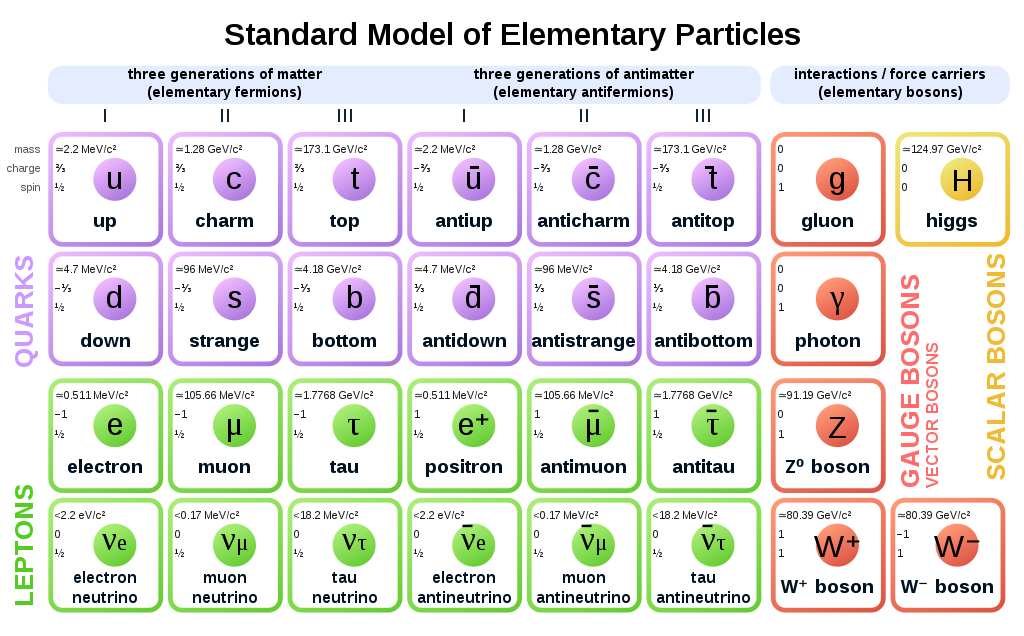
\includegraphics[height=9cm]{1024px-Standard_Model_of_Elementary_Particles_Anti.png}
	\caption{Elementary particles in the Standard Model.\cite{sm_particles}}
	\label{fig:sm-table}
\end{figure}

\begin{comment}
 in a picture where they interact through exchange of certain force carriers which are bosons as well. More specifically, each set of these carriers mediate one type of fundamental interaction. The force in which most of classical objects interact is electromagnetic interaction and it's mediated by photons. The force that plays a role in the $\beta$ decay is weak interaction, of which the mediators are $\textit{W}$ and $\textit{Z}$ bosons. When a proton and a neutron interact within a nuclei transforming into each other, the actual force carriers are 8 types of gluons (or $\pi$ mesons between nucleus), and it's called strong force. Last but not least, in the quantum field theory, all of these particles has zero mass if there's no spontaneous symmetry breaking by introducing one another boson - Higgs boson, in the Lagrangian formalism of all interactions. With this being said, the ``mass'' is taken as the weight of how strong all these particles interact with Higgs field.
 
 However, the S prediction does not perfectly match with experimental observations. Since the day theory was built, generations of particle physics experiments have been searching for evidences beyond the SM, as known as New Physics (NP). New Physics is expected to unfold a more profound truth of nature which hopefully explains these observed mismatches. The studies on these fields naturally draw a large attention from modern physicists, focusing on discovering and explaining the mismatches between the SM predictions and experiments. Among these research fields, the studies of symmetry violations (or called as asymmetries) plays an important role. The studies of symmetries was once the driving force for physicists when building the modern theory about particle physics. It is no wonder that now the violation of symmetries, which  physicists didn't expect to happen , has become the cutting edge research topics for New Physics. 
 
\end{comment}





\section{Symmetry Violation}
Symmetry violation has been one of the focuses in NP studies due to the internal link between symmetries and conservation laws, which makes it a good probe for possible NP theories beyond the SM. When a known symmetry is found to be broken, it usually leads to the discovery of a new theory.


There are three types of discrete symmetric operations which play important roles in particle physics. Charge-conjugation $\textit{C}$ is the operation that turns particle to its anti-particle. Parity transformation $\textit{P}$  is the one that puts a negative sign before all the spatial related vector such as $\overrightarrow{r} \to -\overrightarrow{r}$. The time-reversing operation $\textit{T}$ is to reversely proceed a physical process backward time.  Physicists were convinced that each of these three symmetric operations makes no change to any physics system. However, in 1950s, Lee and Yang \cite{PhysRev.104.254} first questioned that parity symmetry might be broken in weak interactions. They offered a few possible ways to test it and then by Wu \cite{Wu_exp}, an observation on the $\beta$ decay of $^{60}$Co was presented that the electrons emitted from  $^{60}$Co decay prefers the direction of nuclear spin that can be controlled by the external magnetic field. The violation of $P$ symmetry was discovered by this clear evidence. 

\begin{comment}
\begin{figure}[htbp]
\centering
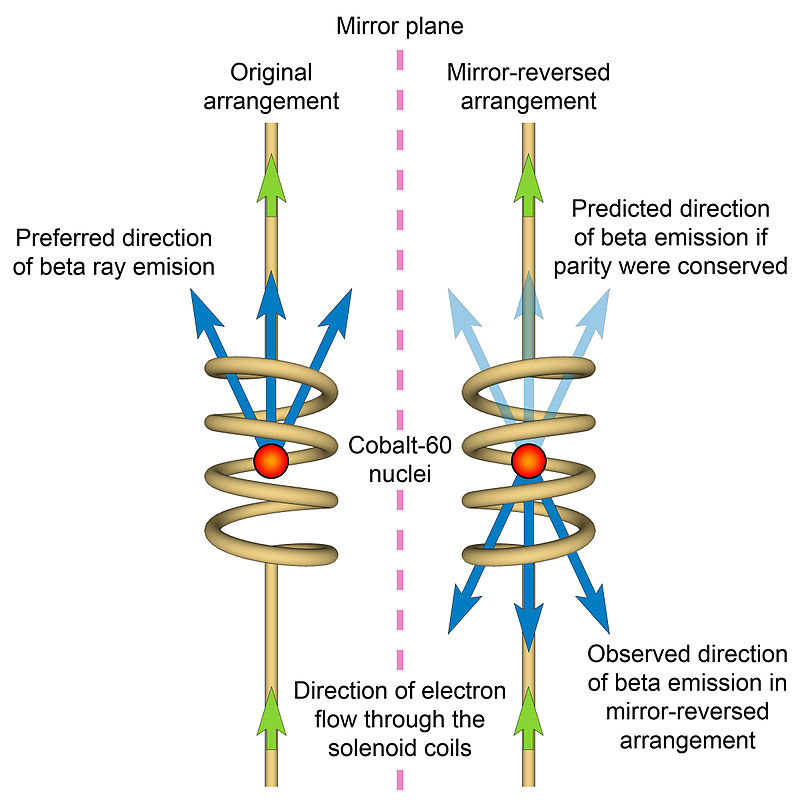
\includegraphics[height=8cm]{DsBxU.jpg}
\caption{$^{60}$Co decay violates the parity because of the unbalance of electron emissions\cite{wu_exp}}
\label{fig:Co60}
\end{figure}
\end{comment}

The first evidence of $CP$ violation was discovered in neutral $K^0$ system by Cronin and Fitch's experiment\cite{christenson1964evidence}. The neutral $K^0$ mesons can be observed as two states that have significantly different lifetime (called as ``$K_S^0$" and ``$K_L^0$" for short and long lifetime particles) with opposite $\it{CP}$ eigenvalue. The experiment measured the decay products at 57 foot of a neutral $K^0$ beamline assuming all the particle at the end of the beam should be long lifetime $K_L^0$, nearly no $K_S^0$. But 0.002\% of $K^0_L$ were found to decay into $\pi^+\pi^-$ which is the main decay process of $K_S^0$.($CP$ eigenvalue $=1$ in $\pi^+\pi^-$ final states, while $K_L$ has  $CP$ eigenvalue $=-1$ ). Given that the expected distance to have 0.002\% of $K_S^0$ at about speed of light is no more than 1 meter in the beamline, such a deviation at 57 foot is an obvious evidence that $K_L^0 \to \pi^+\pi^- $ exists and therefore $CP$ symmetry is violated in the neutral $K^0$ system.

In 1973, Kobayashi and Maskawa introduced a quark mixing matrix called CKM matrix for three or more generations of quarks before the discovery of the third generation of the quark family\cite{CKM}. The theory naturally explained an irreducible complex phase in CKM matrix and it accounts for the origin of $CP$ asymmetries of weak interactions in the Standard Model. The experimental evidence of $CP$ violation in $B$ meson system was observed in 2001 by Belle and BaBar experiments\cite{teramoto2002cp}\cite{langestudy}. They measured the time-dependent decay time difference of $B$ and $\bar{B}$ in the decay of $B\to J/\psi K_S^0$. This channel provided a good clearness in theoretical prediction and has relatively large branching fraction, thus it's called the ``golden mode"\cite{bigi1989question}. In 2008, Kobayashi and Maskawa were rewarded the Nobel Prize to highly value their contribution to $CP$ violation mechanism in the SM, to which Belle experiment contributes greatly. Later in 2010, the upgrade of Belle, Belle II and the upgrade of KEK accelerator, SuperKEKB, were approved to further push the understanding of $CP$ violation along with other topics in New Phsyics researches. 

\section{CKM mechanism}
\begin{comment}
Three kinds of fundamental interaction: weak, strong and electromagnetic interactions have been included in the SM. The SM can inherently solve the origin of the symmetries and asymmetries, with the theoretical support from quantum field theory (QFT). In QFT, the particles are treated as the excitation of its field and the interaction between particles can also be treated as the exchange of energy and momentum between particles. Enlighten by many aspects in classical mechanism, QFT is also built on a formalism in which the Lagrangian plays an essential role. The difference is field, as a physical entity, is universally distributed in space-time, whereas classical objects can only exist with a local position. Given this fact, it is natural to define the Lagrangian of field as a ``density" of Lagrangian of particles. In the SM, for instance, a fermion field $\it{\Psi}$ with mass $m$ is described by a field as follows:

\begin{equation}
\mathcal{L}_0 = \it{\overline{\Psi}(i\gamma^\mu \partial_\mu-m)\Psi}
\end{equation}

Such form presents a field which will fit in Lorentz transition and space-time transition. Then gauge theory is used to describe the interaction of fermions so that the Lagrangian should be invariant under the local gauge transformation. There are different types of local gauge transformations, as well as their invariance. 
Group is the mathematical term used to describe transformation invariance. Each group has a basic presentation of matrix. If every elements in a group can find a corresponding matrix which keeps their relations in multiplying operation,then the smallest dimension of such matrix is called basic matrix presentation. If the matrix elements are Unitary, n dimension, such group is called$\it{U}$(n), 
specially if the anti-matrix is the conjugation-transverse of itself, such group is called Special Unitary.($\it{SU}$(n)) 


For instance, in the U(1) gauge transition, if one requires the invariance of electromagnetism by adding $\it{U}$(1) gauge, the Maxwell formalism naturally fits in the quantum electroweak dynamics (QED), along with the weak interaction which is invariant under not only $\it{U}$(1) transformation but also $\it{SU}$(2). The symmetry of electromagnetic force and weak force is spontaneously broken due to the non-zero expected value of Higgs field of the vacuum. That makes the coupling of different field varied so the carriers of electromagnetic field and weak field diverged. Massless particle $\gamma$ is carrying the electromagnetic force. $W^{+/-}$ and neutral $Z$ deliver the force of weak interaction. They have different coupling strength to the Higgs field, which excites a neutral particle, Higgs boson $H$. The quarks, however, not only coupling to $W^{+/-},Z$ by weak interaction, they directly interact with each other by exchanging gluons by strong force. The strong interaction is described by $SU$(3) with eight types of different gluons, and every gluon has 3 colors. The mechanism that describes this interaction is called ``quantum chromodynamics" (QCD). 

The contribution of the origin of $CP$ violation is mainly from the weak current in the SM Lagrangian. So the discussion of the theoretical interface of $CP$ violation will be focusing on the weak interaction. In the Lagrangian formalism in the SM, gauge interactions are described by the terms in the Lagrangian in a form that quark field is coupling with each other through gauge current, specifically the weak or neutral current. In order to keep the $SU$(2) symmetry treating the quarks from same generation equally, the weak eigenstates are introduced for presenting the Lagrangian. However, if we require the gauge bosons $W^{+/-}$ and $Z$ acquire mass from Yukawa coupling with Higgs field, the term that describes the weak interaction is spontaneously breaking under $CP$ operation. 

\end{comment}


 


\begin{equation}{\label{Eqn:higgs_field}}
\large
\Phi = 
\begin{pmatrix}
\phi^+\\
\nu + \frac{H+i\chi}{\sqrt{2}}
\end{pmatrix}
\end{equation}

 Equation \ref{Eqn:higgs_field} is the Higgs potential doublets in the SM, where the value of $H$ is 174 GeV as the expected Higgs potential for vacuum\cite{sher1989electroweak}. The $\phi$ and $\chi$ are the pseduo-Goldstone fields which are appearing when introducing Higgs field  $\phi$ without breaking the gauge symmetry. The Lagrangian for Yukawa interaction of the quark fields\cite{ceccucci2008ckm} can be presented by Equation \ref{yukawa_coupling}.

\begin{equation}{\label{yukawa_coupling}}
\large
\mathcal{L}_{Yuk}^q = 
-{Q}^\dag Y^d \Phi d_R^\prime 
-{Q}^\dag Y^u \epsilon \Phi^* u_R^\prime
+ h.c.
\end{equation}

where the primed fields stand for the weak eigenstates of quarks. The $\epsilon$ is a 2$\times$ 2 matrix and $Q^\dag$ is the left-handed doublets that stand for weak eigenstates of up and down types quarks, see Equation \ref{eq:eps} and \ref{eq:qdag}. 

\begin{equation}\label{eq:eps}
\epsilon =  
\begin{pmatrix}
0 & 1\\
-1 & 0
\end{pmatrix}
\end{equation}

\begin{equation}\label{eq:qdag}
Q =  
\begin{pmatrix}
u^\prime & d^\prime \\
c^\prime & s^\prime \\
t^\prime & b^\prime
\end{pmatrix}_L
\end{equation}

Yukawa matrix is an arbitrary 3 $\times$ 3 complex matrix $Y^{u,d}$ which gives the rise of up and down type massive quark field $M^{u,d}=Y^{u,d}\nu$ according to Equation \ref{yukawa_coupling}. The representation of the quark fields using weak eigenstates can be transformed to mass eigenstates by Equation \ref{rot1} and \ref{rot2}.

\begin{equation}\label{rot1}
S_{L,R}^{u}
\begin{pmatrix}
u^\prime   \\
c^\prime  \\
t^\prime 
\end{pmatrix}_{L,R}
= \begin{pmatrix}
u  \\
c  \\
t 
\end{pmatrix}_{L,R}
\end{equation}

\begin{equation}\label{rot2}
S_{L,R}^{d}
\begin{pmatrix}
d^\prime   \\
s^\prime  \\
b^\prime 
\end{pmatrix}_{L,R}
= \begin{pmatrix}
d  \\
s  \\
b 
\end{pmatrix}_{L,R}
\end{equation}


 In Equation \ref{rot1} and \ref{rot2}, $S^{u,d}_{L,R}$ are all unitary matrices since they are generated by the normalized eigenstate states of Yukawa matrix. The mass
  item in the Lagrangian can be presented as Equation \ref{eq:Mq}
\begin{equation}\label{eq:Mq}
\mathcal{L}_{m} = -\sum_{q=u,c,t,d,s,b}^{} M_q q^{\dag}_{} q_{}
\end{equation}
where the $q=(q_L+q_R)$ is four-component Dirac field, and $q_L^\dag q_L = q_R^\dag q_R = 0$. 
As a result of diagonalizing $Y^{u,d}$,  the charged current $W^{\pm}$ interactions coupe to the physical quarks and the Lagrangian is written as Equation \ref{weak_coupling}, where $V_{CKM} \equiv S_L^u S_L^{d\dag}$.

\begin{equation}\label{weak_coupling}
\small
\mathcal{L}^q_W = \frac{g}{\sqrt{2}}
\begin{bmatrix}
\begin{pmatrix}
\overline{u}&\overline{c}&\overline{t}
\end{pmatrix}_L

\gamma^\mu W^{+}_{\mu}
%{S^{u}_{L}}^{\dag}
%S^{d}_{L}
V_{CKM}
\begin{pmatrix}
d\\s\\b\\
\end{pmatrix}_L+
\begin{pmatrix}
\overline{d}&\overline{s}&\overline{b}
\end{pmatrix}_L
\gamma^\mu W^{-}_{\mu}
%S^{u}_{L}
%{S^{d}_{L}}^{\dag}
V_{CKM}^{\dag}
\begin{pmatrix}
u\\c\\t\\
\end{pmatrix}_L
\end{bmatrix}
\end{equation}

%\begin{equation}
%V_{CKM} = 
%{S^{u}_{L}}^{\dag}
%S^{d}_{L}
%\end{equation}

% 2020.02.12 mid 
The Lagrangian hereby clearly declares the transition of different charged quarks through the coupling of charged current $W^{\pm}$, where such a coupling only applies for the left-handed quarks. For example, a left-handed charm quark only transits to left-handed strange quark by a $W$ boson. By only applying $C$ or $P$ conjugation, the Lagrangian is not invariant, indicating the non-conservation of $C$ or $P$ individually. However, if the $CP$ conjugation is applied, the Equation \ref{weak_coupling} transits as Equation \ref{cp-conj} shows.
\begin{equation}\label{cp-conj}
\small
\large
\begin{pmatrix}
\overline{u}&\overline{c}&\overline{t}
\end{pmatrix}_L
\gamma^\mu W^{+}_{\mu}
V_{CKM}
\begin{pmatrix}
d\\s\\b\\
\end{pmatrix}_L
{\Leftrightarrow}
\begin{pmatrix}
{u}&{c}&{t}
\end{pmatrix}_L
\gamma^\mu W^{-}_{\mu}
{V_{CKM}}
\begin{pmatrix}
\overline d\\\overline s\\\overline b\\
\end{pmatrix}_L
\end{equation} 

Comparing  Equation \ref{cp-conj} and \ref{weak_coupling}, the $\it{CP}$ symmetry requires the invariance before and after $CP$ conjugation, meaning that Equation \ref{cp_cons} is expected.

\begin{equation}\label{cp_cons}
\large
{u_{L}^i}V_{ij} \bar{d}^{j}_L \gamma^\mu W^{-}_{\mu}
=
{{u}^{n}_LV^{*}_{nm}\bar{d}_{L}^m}  \gamma^\mu W^{-}_{\mu}
\end{equation}
The same indices $ij$ and $nm$ are summed over on both side. This is equivalent to Equation \ref{v-eq}: 
\begin{equation}\label{v-eq}
V_{ij} = V^{*}_{ij}
\end{equation}
On the one hand, if the CKM matrix is real, $CP$ will be conserved in the weak interaction in the SM due to the natural hold of Equation \ref{v-eq}. On the other hand, from Equation \ref{cp_cons}, it's still possible to make Lagrangian invariant even if $V_{CKM}$ is not real, which can be achieved by introducing non-physical phases for each quark field $u^k_L e^{(i\phi_{uk})}$ and $d^j_L e^{(i\phi_{dj})}$, the Equation \ref{v-eq} becomes Equation \ref{eq:ckm_phase}.
\begin{equation}\label{eq:ckm_phase}
\Large
V_{kj} e^{i(\phi_{dj}-\phi_{uk})} = V^{*}_{kj}e^{i(\phi_{uk}-\phi_{dj})}
\end{equation}

Assuming the complex phase of the $kj$-th element in CKM matrix is $\theta_{kj}$, it's obviously required Equation \ref{eq:ckm_phaseeq} to hold.
\begin{equation}\label{eq:ckm_phaseeq}
\large
\theta_{kj} = \phi_{uk}-\phi_{dj}
\end{equation}
If the number of generations in quark family is 3 or more, the non-physical phases can not render proper values to ensure the hold of Equation \ref{eq:ckm_phaseeq}, and there will always be one irreducible complex phase parameter in the CKM matrix in the existence of three generations of quarks, which means $\it{CP}$ symmetry is no longer conserved in the weak interactions. 

The $3\times 3$ unitary CKM matrix can be written as Equation \ref{CKM} based on the quark fields it connects using Equation \ref{rot1} and \ref{rot2}.
\begin{equation}\label{CKM}
\large
V_{CKM}=
\begin{pmatrix}
V_{ud} & V_{us} & V_{ub}\\
V_{cd} & V_{cs} & V_{cb}\\
V_{td} & V_{ts} & V_{tb}\\
\end{pmatrix}
\end{equation}

It can be parameterized into the form of Equation \ref{eq:ckm_par}.
\begin{equation}\label{eq:ckm_par}
V_{CKM}=
\begin{pmatrix}
c_{12}c_{13} & s_{12}c_{13} & s_{13}e^{-i\delta }\\
-s_{12}c_{23}-c_{12}s_{23}s_{13}e^{-i\delta } &c_{12}c_{23}-s_{12}s_{23}s_{13}e^{-i\delta } & s_{23}c_{13}\\
s_{12}s_{23}-c_{12}s_{23}s_{13}e^{-i\delta }  & -c_{12}c_{23}-s_{12}c_{23}s_{13}e^{-i\delta } & c_{23}c_{13}
\end{pmatrix}
\end{equation}
where the $c_{jk}=\text{cos}(\theta_{jk})$ and $s_{jk}=\text{sin}(\theta_{jk})$, and $\delta$ is the irreducible complex phase. By measuring the relative branching ratio of $b\to c$, $s\to u$ and $b\to u$ in tree level transitions as shown in Equation \ref{eq:ckm_larger}.
\begin{equation}\label{eq:ckm_larger}
|V_{ub}|\ll |V_{cb}|\ll |V_{us}|
\end{equation}

The relations in Equation \ref{ckm_par1} are often used to simplify CKM matrix presentation.
\begin{equation}\label{ckm_par1}
s_{13}=\lambda , s_{23}=A\lambda^2, s_{13}e^{i\delta}=A\lambda^3(\rho-i\eta)
\end{equation}
% 2021.01.23 ends 
By using Equation \ref{ckm_par1}, CKM matrix is parameterized as Equation \ref{eq:ckm_lambda}.
\begin{equation}\label{eq:ckm_lambda}
V_{CKM}=
\begin{pmatrix}
1-1/2\lambda^2 & \lambda & A\lambda^3(\rho-i\eta)\\
-\lambda & 1-1/2\lambda^2 & A\lambda^2\\
A\lambda^3(\rho-i\eta) & -A\lambda^2 & 1
\end{pmatrix}+\mathcal{O}(\lambda^4)
\end{equation}

Using the unitary condition, the Equation\ref{ckm_triangles} is obtained.
\begin{equation}\label{ckm_triangles}
1+
\frac{V_{ud}V^*_{ub}}{V_{cd}V^*_{cb}}+
\frac{V_{td}V^*_{tb}}{V_{cd}V^*_{cb}}
=0
\end{equation}
Using Equation \ref{ckm_triangles}, \ref{eq:ckm-rho1} and \ref{eq:ckm-rho2}, the shape of CKM triangle can be defined on the complex plane in Figure \ref{fig:ckm_angles}.
\begin{figure}[htpb]
	\centering
	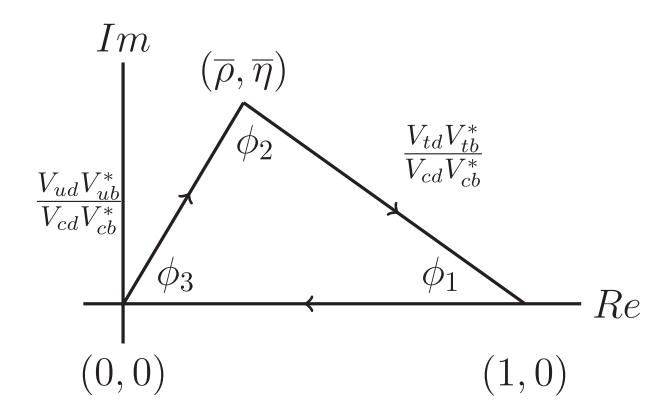
\includegraphics[height=6cm]{UT}
	\caption{The unitary triangles of CKM\cite{ckmfitter}.}
	\label{fig:ckm_angles}
\end{figure}
\begin{eqnarray}
\bar{\rho}+i\bar{\eta}=- \frac{V_{ud}V^*_{ub}}{V_{cd}V^*_{cb}}\label{eq:ckm-rho1}\\
1-(\bar{\rho}+i\bar{\eta})=-\frac{V_{td}V^*_{tb}}{V_{cd}V^*_{cb}}\label{eq:ckm-rho2}
\end{eqnarray}
These angles are obtained by drawing the $(\bar{\rho},\bar{\eta})$ on the complex coordinates, and they are also well-known in the names as: $\phi_1=\beta,\phi_2=\alpha,\phi_3=\gamma$. The results presenting the measurement of CKM angles or $(\bar{\rho},\bar{\eta})$ in 2019 are shown in Figure \ref{fig:ckm19}.
\begin{figure}[htbp]
	\centering
	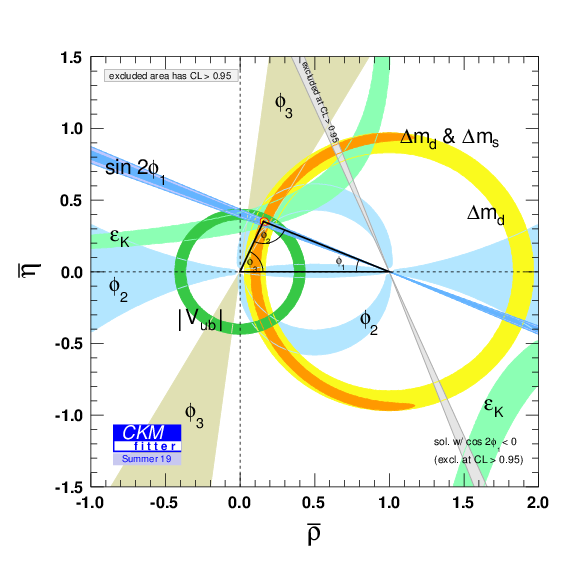
\includegraphics[height=8cm]{ckm19}
	\caption{The CKM triangle fit in the complex plane of $\bar{\rho}-\bar{\eta}$.\cite{ckmfitter}}
	\label{fig:ckm19}
\end{figure}

The measurement of $\phi_1$ and $\phi_2$ are mainly obtained from the time-dependent $CP$ violations (TDCPV) measurement. The $\phi_1$ in the tree-level dominated decays has been precisely measured due to the small hadronic uncertainties. Flavor-Changing-Neutral-Current (FCNC) processes can rise through the $B^0_d-\bar{B^0_d}$ mixing in box diagram, and it's believed that potential NP processes might contribute to the difference in between results of CKM angles measured from experiments, such as $\phi_1$ value in tree-dominated processes and penguin-dominated processes, where both involve $b\to s$ transition. It requires the precise measurements on multiple decay channels to search for the potential NP effects. The prospective large Belle II data and improved detector performance will be much useful to help the discovery of NP in future. 

\section{Time Dependent $CP$ violation}
\subsection{ $CP$ violation in neutral $B$ system}
The  $\phi_1$, $\phi_2$ and $\phi_3$ are essentially measuring the CKM $CP$ violating phase since there's only one complex phase in the CKM matrix and it can be determined by these three angles. 
For determining the value of $\phi_1$, TDCPV measurements provide a good experimental environment.  
From Figure \ref{fig:ckm_angles}, one can obtain $\phi_1$ and $\phi_2$ by Equation \ref{eq:phi1} and \ref{eq:phi2}.
\begin{eqnarray}
\phi_1=Arg(-\frac{V_{td}V^*_{tb}}{V_{cd}V^*_{cb}}) \label{eq:phi1}\\
\phi_2=Arg(-\frac{V_{td}V^*_{tb}}{V_{ud}V^*_{ub}})\label{eq:phi2}
\end{eqnarray}

The time-dependent $CP$ violation comes from the interference of neutral $B$ mixing phase and the weak phase in the decay amplitude. The mass eigenstates which are driving the propagation of neutral $B$ meson states with mixing are: $|B\rangle_{H,L}=p|B\rangle \pm q|\overline{B}\rangle $, where $H$ and $L$ stand for the heavier and lighter mass eigenvalues. The $|B\rangle$ and $|\overline{B}\rangle$ present the flavor eigenstates of neutral $B$ mesons.
The Hamiltonian matrix can be written using flavor eigenstates as shown in Equation \ref{eq:ham_flv}.
\begin{equation}\label{eq:ham_flv}
M_\Gamma=
\begin{bmatrix}
m-i/2\Gamma & M_{12}-i/2\Gamma_{12}\\
M^*_{12}-i/2\Gamma^*_{12}& m-i/2\Gamma 
\end{bmatrix}
\end{equation}
Considering the time evolution of mass eigenstates, the time-dependent states can be shown as Equation \ref{eq:Bht} and \ref{eq:Blt} by using the notation of $B_{H,L}$ as physical states at $t = 0$).
\begin{eqnarray}
B_H(t)=e^{-im_Ht}e^{-\Gamma_Ht/2}B_H \label{eq:Bht}\\
B_L(t)=e^{-im_Lt}e^{-\Gamma_Lt/2}B_L\label{eq:Blt}
\end{eqnarray}
where $M_{H,L}$ and $\Gamma_{H,L}$ are the masses and decay widths of two mass eigenstates. By expanding the mass eigenstates using flavor eigenstates, which are shown in Equation \ref{Bt} and \ref{Bbart}.
\begin{eqnarray}
B(t)=(1/2p)e^{-im_Ht}e^{-\Gamma_Ht/2}(pB+q\bar{B})+(1/2p)e^{-im_Lt}e^{-\Gamma_Lt/2}(pB-q\bar{B}) \label{Bt}\\
\bar{B}(t)=(1/2q)e^{-im_Ht}e^{-\Gamma_Ht/2}(pB+q\bar{B})-(1/2q)e^{-im_Lt}e^{-\Gamma_Lt/2}(pB-q\bar{B})\label{Bbart}
\end{eqnarray}
Replacing $g_{\pm}(t)=\frac{1}{2}(e^{-im_Ht-\Gamma_H/2t}\pm e^{-im_Lt-\Gamma_L/2t})$, Equation \ref{Bt} and \ref{Bbart} become Equation \ref{eq:Bt_new} and \ref{eq:Bbart_new}.
\begin{eqnarray}
B(t)=g_{+}(t)B +\frac{q}{p}g_{-}(t)\bar{B} \label{eq:Bt_new}\\
\bar{B}(t)=g_{+}(t)\bar{B} + \frac{p}{q}g_{-}(t){B}\label{eq:Bbart_new}
\end{eqnarray}
Considering all the phase-spaces of the decay from flavor eigenstates to final states $f(\bar{f})$ are included in the amplitudes $\mathcal{A}_f (\bar{\mathcal{A}}_f)$, one needs to expand the flavor eigenstates using the final states amplitudes to have the differential decay rate $\Gamma(B\to f,t)$. From $B(t) \propto \mathcal{A}_f\psi_f+h.c $ and $ (\bar{B}(t) \propto \bar{\mathcal{A}_f}\psi_{\bar{f}}+h.c)$, combined with Equation \ref{eq:Bt_new} and \ref{eq:Bbart_new}, the decay rate can be shown in Equation \ref{eq:gamma_B} and \ref{eq:gamma_Bbar}.
\begin{eqnarray}
\Gamma(B\to f,t)=|\mathcal{A}_f|(|g_+(t)|^2+|\lambda_f|^2|g_-(t)|^2+2Re(\lambda_f g^*_+(t)g_-(t))) \label{eq:gamma_B}\\
\Gamma(\bar{B}\to \bar{f},t)=|\bar{\mathcal{A}_{\bar{f}}}|(|g_+(t)|^2+|\bar{\lambda}_{\bar{f}}|^2|g_-(t)|^2+2Re(\bar{\lambda}_{\bar{f}} g^*_+(t)g_-(t)))\label{eq:gamma_Bbar}
\end{eqnarray} where the parameter $\lambda_f$ and $\bar{\lambda}_{\bar{f}}$ can be defined as Equation \ref{eq:lambda_f} and \ref{eq:lambda_fbar}.
\begin{eqnarray}
\lambda_f \equiv (q/p) (\bar{\mathcal{A}}_f / \mathcal{A}_f) \label{eq:lambda_f}\\
\bar{\lambda}_{\bar{f}} \equiv (q/p) ( \mathcal{A}_{\bar{f}}/\bar{\mathcal{A}}_{\bar{f})} \label{eq:lambda_fbar}
\end{eqnarray} 
The $q/p$ is introduced by the coefficient of mass eigenstates from weak eigenstates. Using the Hamiltonian matrix, $q/p$ can be presented using Equation \ref{eq:qp}
\begin{equation}\label{eq:qp}
	q/p = \frac{\Delta M - i/2 \Delta \Gamma}{2(M_{12}- i/2 \Gamma_{12})}
\end{equation}
where the $M_{12}$ and $\Gamma_{12}$ stands for the contribution of non-diagnosed term in the Hamiltonian matirx. $\Delta{M}=M_H-M_L$ and $\Delta{\Gamma}=\Gamma_H-\Gamma_L$ are the difference of mass and decay width for two mass eigenstates, respectively.
It's obvious that if $|A_f| \neq |\bar{A}_{\bar{f}}|$, direct $\it{CP}$ violation will occur.  
The time-dependent decay rate difference is defined as Equation \ref{Acp}.
\begin{equation}\label{Acp}
\begin{split}
A_{CP}(t)&\equiv \frac{\Gamma(B\to f,t)-\Gamma(\bar{B}\to \bar{f},t)}{\Gamma(B\to f,t)+\Gamma(\bar{B}\to \bar{f},t)}\\
&=\frac{\mathcal{S} sin(\Delta{M}t)-\mathcal{A}cos(\Delta{M}t)}
{cosh(\Delta \Gamma t/2)+A^f_{\Delta \Gamma}sinh(\Delta \Gamma t/2)}
\end{split}
\end{equation}
where
\begin{eqnarray}\label{cp-parameters}
\mathcal{S}=\frac{2Im(\lambda_f)}{1+|\lambda_f|^2} \label{eq:S}\\
\mathcal{A}=\frac{1-|\lambda_f|^2}{1+|\lambda_f|^2}\label{eq:A}\\
A^f_{\Delta \Gamma}=-\frac{2Re(\lambda_f)}{1+|\lambda_f|^2}
\end{eqnarray}
From Equation \ref{eq:S} and \ref{eq:A}, the time-dependent CP violation parameters $\mathcal{S}$ and $\mathcal{A}$ are dependent on the parameter $\lambda_f$.

\subsection{$\phi_1$  from $B^0 \to J/\psi K^0_S$}
If final states are $CP$ eigenstates, the amplitudes are obtained by $\mathcal{A}_f \equiv \langle f|H|B\rangle$ and $\bar{\mathcal{A}_f} \equiv \langle f|H|\bar{B}\rangle$. In $B_d^0-\bar{B_d^0}$ mixing system, the $q/p$ can be treated as $e^{i\phi_d}$ as a pure phase term. This relative phase accounts the transition from $b$ to up-type quarks to strange quark $s$ in mixing, so it can be presented as $\phi_d = \text{Arg}(V^*_{td}V_{tb})/(V^*_{tb}V_{td}) \approx 2\phi_1 $ based on negligible correction to the SM. In mode $B^0 \to J/\psi K^0_S$, considering $\Delta \Gamma$ can be treated as zero in the SM in this case\cite{dighe2001width}, Equation \ref{Acp} can be reduced to Equation \ref{eq:acp}.

\begin{equation}\label{eq:acp}
	A_{CP}(t)=\mathcal{S} \text{sin}(\Delta{M}t)- \mathcal{A}\text{cos}(\Delta{M}t)
\end{equation}

\begin{comment}
Usually, $S_f$ provides a good sensitivity to $\phi_1$ in Eq(1.42) by replacing $\phi_d$ inside $\lambda_f$ since the rest two equations canceled out the complex phase of $(q/p)$. For instance, in the process of  $b\to \bar{c}cs$ ,the amplitude contributions from tree level and loop level diagram can be written in a form as follows using the CKM unitary condition: 
\end{comment}
which receives contributions from tree-level and loop-level processes shown in Figure \ref{fig:jpsiks} , 

\begin{figure}[htpb]
	\centering
	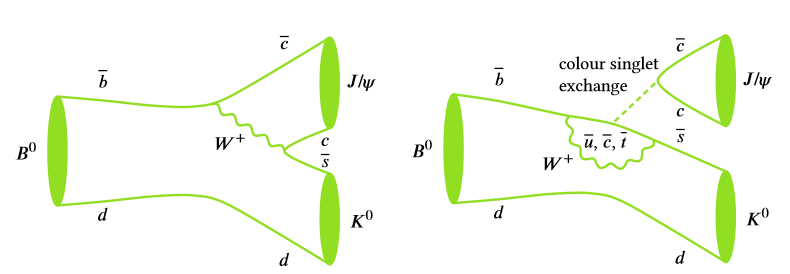
\includegraphics[height=4cm]{jpsiks-diagram}
	\caption{The dominated tree-level (left) and the suppressed loop-level (right) of $B\to J/\psi K^0$, in which $K^0$ particles are detected $K_S^0$\cite{wishahi2014measurement}.}
	\label{fig:jpsiks}
\end{figure}

%\begin{equation}
%	\mathcal{A}_f= 
%	\lambda^s_c T_f + 
%	\lambda^s_u P_f; \\
%	\lambda^q_i = V^*_{ib}V_{iq}
%\end{equation}
%where $T_f$ and $P_f$ stands for leading order contribution of tree and penguin diagrams, see Fig(1-7). Here, the leading term can be presented as: 

Using the relation $|V_{ub}|\ll |V_{cb}|\ll|V_{us}|<|V_{cs}|$, it's obvious that $V^*_{ub}V_{us} \ll V^*_{cb}V_{cs}$, so the penguin-mode is suppressed in the Standard Model. The $\eta_f$ is defined as the $\it{CP}$ eigenvalue. Given $\eta_f=1$ and $|\lambda_f|=1$ in $B^0 \to J/\psi K^0_S$, from \ref{cp-parameters}, $\it{CP}$ violation parameters can be presented as shown in Equation \ref{SA}.
\begin{equation}\label{SA}
\mathcal{S} = Im(\lambda_f)
=-sin(\phi_d)\eta_f=-sin(2\phi_1) ; \: \mathcal{A} = 0
\end{equation}

From Equation \ref{SA} , $\phi_1$ can be obtained precisely in the measurement of time-dependent $\it{CP}$ violation in $B^0 \to J/\psi K^0_S$.
\begin{comment}
In the $b\to q\bar{q}s$ process where flavor $q$ is not charm, similar to the discussion above, we can extract $\phi_1$ using the same method. Moreover, it provides a penguin-dominated process which is sensitive to the contribution of New Physics, which includes the $B^0_d\to K^0_S K^0_S K^0_S$ decay. In the next section, it's clear that such decay process is important to provide additional insight in seeking the effect beyond the SM (BSM contribution).
\end{comment}



\subsection{$\phi_1$ from penguin-dominated mode $b\to q\bar{q}s$}
Compared to $B^0 \to J/\psi K^0_S$ channel, the measurement of $\mathcal{S}$ and $\mathcal{A}$ from penguin-dominated channels through $b \to q\bar{q}s$ where $q$ is $u,d,s$ can be different due to the varied tree-to-penguin amplitude ratio. Furthermore, they are quite sensitive to NP effects for the following reasons\cite{b2book}. First, they can probe $B^0-\bar{B}^0$ mixing through different short-distance vertices compared to the tree-level dominated decays. Second, the tree-level decay amplitude is suppressed and penguin-level amplitude is dominated, while the overall non-NP amplitude is relatively small so NP effects may show up easier. Last but not least, they comprise a large number of different final states, which can help disentangling non-perturbation long-distance physics from short-distance information, such as $\phi_1$ or NP contributions to the weak Hamiltonian. 

\begin{comment}
First,  the $b\to q\bar{q}s$  gives a different vertex in gluonic decay than tree diagram. 
Second, such process is tree level suppressed but penguin-dominated, so the New Physics effects can be easier to be spotted. The SM agrees with tree level process in percent accuracy so the sub-percent BSM effects may be hard to see. Similar to Fig(1-7), due to FCNC tree level forbidden, 
\begin{figure}[H]
\centering
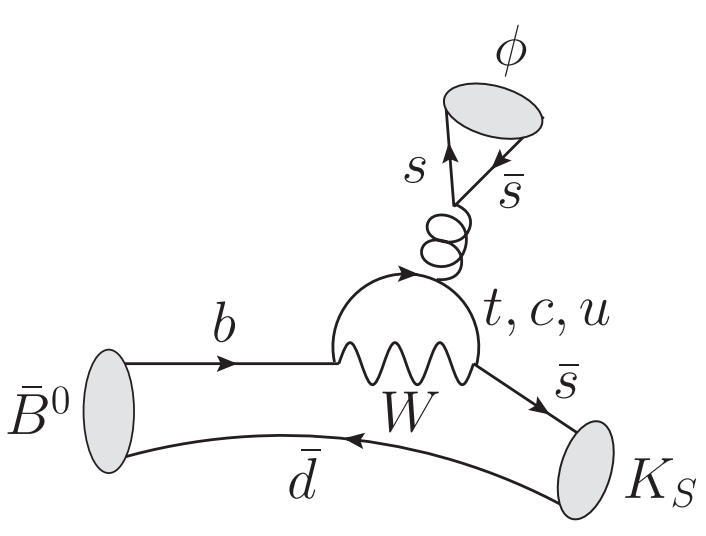
\includegraphics[height=5cm]{Bto3Ks}
\caption{penguin mode $b\to q\bar{q}s$ where $\phi$ is formed by two strange quark as the intermediate state.}
\end{figure}

\end{comment}
Considering possible New Physics contribution besides the tree-level and penguin-level processes as $A_f^{NP}$, the decay amplitude can be rendered as Equation \ref{eq:Af_NP} 
\begin{equation}\label{eq:Af_NP}
\mathcal{A}_f= 
\lambda^s_u T_f + 
\lambda^s_c P_f +
{A}_f^{NP} 
\end{equation}
where $T_f$ and $P_f$ are tree-level and penguin-level amplitudes. The coefficients $\lambda^s_u$ and $\lambda^s_c$  are determined from CKM matrix elements by $\lambda^q_i \equiv V^*_{ib}V_{iq}$. Note that compared to the $B^0 \to J/\psi K^0_S$,
the tree level amplitude $T_f$ is suppressed and penguin amplitude $P_f$ is dominated in $b\to q\bar{q}s$. It is also worth noting that $T_f$ contains tree-level $W^{\pm}$ exchange, QCD and electroweak penguin contributions. These carry the combination of CKM matrix elements $\lambda_t^s = V_{ts}V^*_{tb}=-(1+\epsilon_{uc})\lambda^s_c$ where $\epsilon_{uc} \equiv \lambda^s_u / \lambda^s_c = \mathcal{O}(\lambda^2)$. In the SM with neglected $\epsilon$,  $b\to q\bar{q}s$ modes are pure penguin with the same weak phase as $B^0 \to J/\psi K^0_S$ has. Thus, direct $CP$ violation vanishes and time-dependent $CP$ violation reflects $\mathcal{S}$ in the same way as $B^0 \to J/\psi K^0_S$ does. 

Departures from this limit, non-neglected tree amplitude $T_f$ (often called ``tree pollution"), as well as possible NP effects, could give different results on $\phi_1$. Introducing the tree-penguin ratio $r^T_f = T_f / P_f$, NP-to-SM ratio $r^{NP}_f = \mathcal{A}^{NP}_f / (\lambda^s_c P_f)$, the following statements are usually used\cite{b2book}:

\textbullet \space Branching ratios are affected at $\mathcal{O}(|\epsilon_{uc}r^T_f|,|r^{NP}_f|)$

\textbullet \space Direct CP violation in the SM are of $\mathcal{O}(\epsilon_{uc}\text{Im}(r^T_f))$


\textbullet \space $-n^{CP}_f\mathcal{S} = \text{sin}(2\phi_1) + \Delta \mathcal{S}$, where
$\Delta \mathcal{S}=2{cos}2\phi_1 {sin}\phi_3 |\epsilon_{uc}| \text{Re}(r^t_f) + \Delta \mathcal{S}^{NP}$


\subsection{$\phi_1$ from $B^0 \to K_S^0  K_S^0  K_S^0$}% 2021.01.25 ends
Since the Belle experiment reported the time-dependent $\it{CP}$ analysis on various $b\to q\bar{q}s$ which experimentally showed that the difference on $\phi_1$ has a margin for NP effects\cite{chen2007observation}, the improved measurements with a larger data collection is popularly discussed in order to reduce the impact of uncertainties and clear the tension between results. The decay channel $B^0 \to K_S^0  K_S^0  K_S^0$ is one of the most promising modes for this purpose. The $\it{CP}$ eigenvalue of $B^0 \to K_S^0  K_S^0  K_S^0$ is positive ($CP$ eigenvale $=+1$).  There's no up-quark shown in the final states, the potential contribution of $b\to u\bar{u}s$ re-scattered into $b\to s\bar{s}s$ is almost of absence, which makes $B^0 \to K_S^0  K_S^0  K_S^0$ a much cleaner channel compared to $B^0 \to K^+  K^-  K_S^0$\cite{gershon2004time}. In all final states with three $K_S^0$ from a neutral $B$ decay, the phase-space based decay process and the resonant decay process such as $B^0\to f_0(980)K_S^0(f_0(980)\to K_S^0 K_S^0)$ are shown in the left and middle of Figure \ref{fig:3ksfey}, which all yield $\it{CP}$-even states treated as signal events. In the meanwhile, $b\to c \to s$ can also produce the final states with three $K_S^0$ through a tree-level process like $B^0\to \chi_{c0}K_S^0(\chi_{c0}\to K_S^0 K_S^0)$ with a different weak phase and $\it{CP}$-odd states, as shown in the right of Figure \ref{fig:3ksfey}. Such a tree-level process is treated as background and can be rejected by applying veto on two $K_S^0$ invariant mass within $\chi_{c0}$ mass window, which is considered as a minor background at the current luminosity. Due to the same weak phase in the decay amplitudes, any potential NP effects expected in the $B^0 \to \phi K^0_S$ should also affect $B^0 \to K_S^0  K_S^0  K_S^0$ and the absence of NP effects will lead the same $\it{CP}$ violation just  as $J/\psi K^0_S$\cite{gershon2004time}. Currently there's no specific theoretical calculation on the $\Delta \mathcal{S}$ for three-body $B^0 \to K_S^0  K_S^0  K_S^0$. However, due to the same weak phase of this decay as $\eta^{'} K^0_S$ and $\phi K^0_S$, the theoretical prediction on $\Delta \mathcal{S}$ is usually applied to $B^0 \to K_S^0  K_S^0  K_S^0$ as well\cite{gershon2004time}. The expected range on $\Delta \mathcal{S}$ is typically at level of  $\sim 0.05$\cite{beneke2005corrections}, which requires the expected precision improvement for both statistical and systematic uncertainty in future data.

 \begin{figure}[htpb]
 	\centering
	\begin{minipage}[t]{0.32\linewidth}
		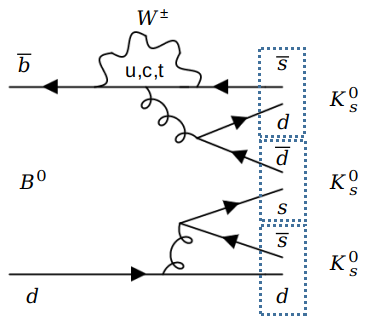
\includegraphics[width=1\linewidth]{fey1}
	\end{minipage}
	\begin{minipage}[t]{0.32\linewidth}
		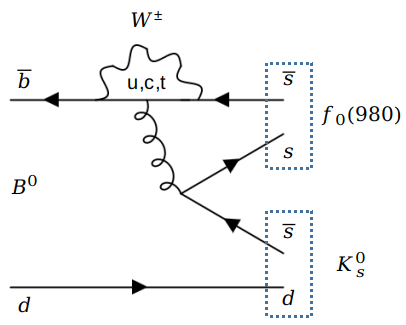
\includegraphics[width=1\linewidth]{fey2}
	\end{minipage}
\begin{minipage}[t]{0.32\linewidth}
	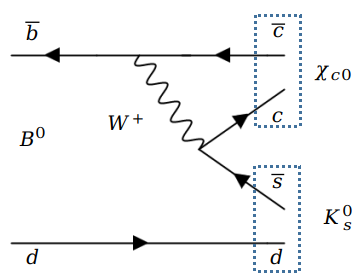
\includegraphics[width=1\linewidth]{fey3}
\end{minipage}
	\caption{}
	\label{fig:3ksfey}
\end{figure}

The result of $\phi_1$ from $B^0 \to J/\psi K_S^0$ using the full Belle data is presented as $\mathcal{S}_{J/\psi K^0_S} = + 0.670 \pm 0.029 (\text{stat}) \pm 0.013(\text{syst})$\cite{b2book}. In the meantime, the latest result of  $\phi_1$ from $B^0 \to K_S^0  K_S^0  K_S^0$ using the full Belle data\cite{kang2020measurement} is presented as: $\mathcal{S}_{3K^0_S} = - 0.71 \pm 0.23 (\text{stat}) \pm 0.05(\text{syst})$, and the result from BaBar \cite{Lees:2011nf} is: $\mathcal{S}_{ 3K^0_S} = - 0.94 ^{+0.21}_{-0.24} (\text{stat}) \pm 0.06(\text{syst})$. Both results have shown a small deviation from the result in $B^0 \to J/\psi K_S^0$ while the statistical uncertainties are much dominated which prevents the claim about whether NP effects are existed. For $\Delta \mathcal{S}$ from $B^0 \to K_S^0  K_S^0  K_S^0$, the experimental sensitivity of $\Delta \mathcal{S}$ will be dominated by $\mathcal{S}_{3K^0_S}$ because the total uncertainty from $J/\psi K^0_S$ will be reduced to  $\sim0.005$ at $50 \: \text{ab}^{-1}$ Belle II data\cite{b2book}. The Figure \ref{fig:sensitivity} shows the scaled $\Delta \mathcal{S}$ sensitivity from the Belle II technical design report\cite{Abe:2010gxa} with respect to the luminosity in future Belle II\cite{Abe:2010gxa}, which only includes the statistical uncertainty of Table \ref{tab:sensitivity}. If the conservative estimation based systematic uncertainty from Belle is considered, the red arrow shows the approximate luminosity where the experimental sensitivity becomes comparable with theoretical prediction upper limit at $\sim 0.05$\cite{b2book}. If the center value of future result on $\mathcal{S}$ is shifted away from the one obtained in $B^0 \to J/\psi K^0_S$ by $\sim 0.05$ including a 5 times total uncertainty, then it can be an clear evidence for NP effects. Surely, smaller the total uncertainty is, easier identifying the existence of NP effects will be.

\begin{figure}[H]
	\centering
	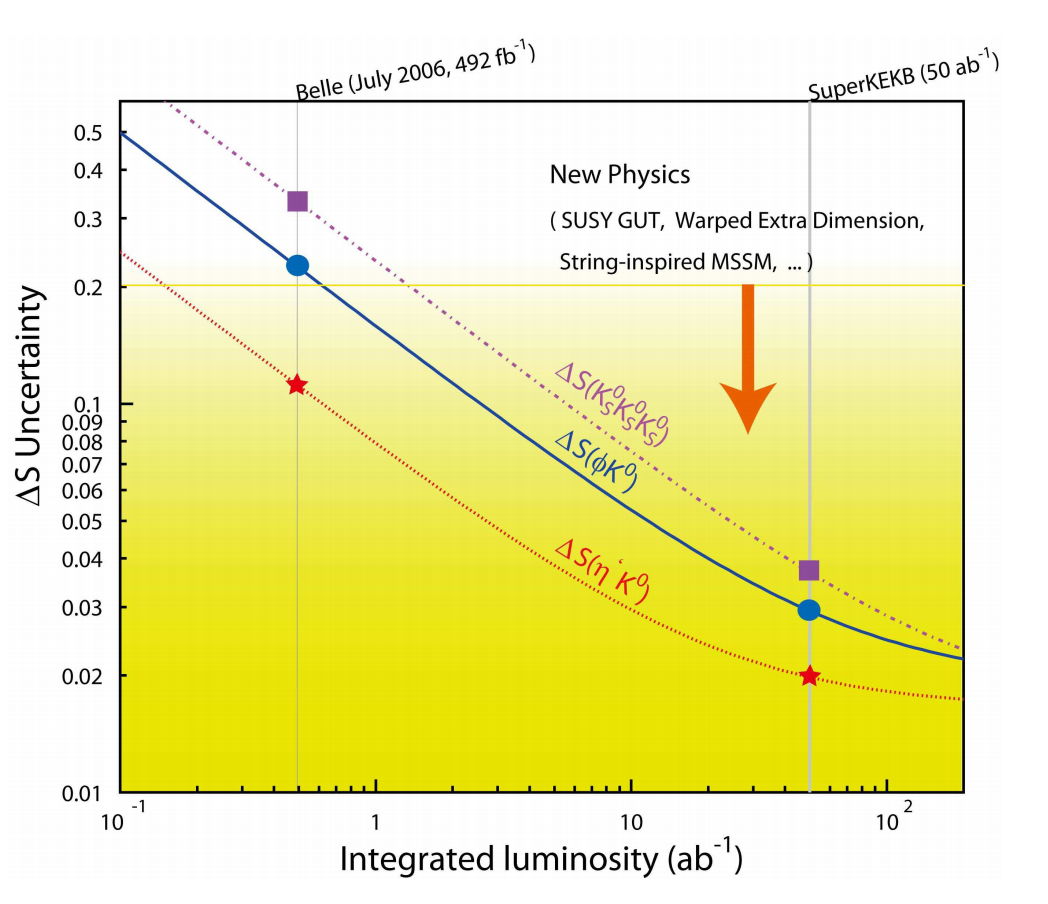
\includegraphics[height=10cm]{sensitivity}
	\caption{Expected  sensitivity of $\Delta \mathcal{S}$ with respect to the integrated luminosity of the Belle II future data from the Belle II technical design report\cite{Abe:2010gxa}.}
	\label{fig:sensitivity}
\end{figure}

\begin{table}[H]
	\centering
	\large
	\caption{$\Delta \mathcal{S}$ estimated statistical uncertainties with respect to the integral luminosities in the Belle II technical design report\cite{Abe:2010gxa}. Three decay modes receive the same potential NP effects due to the same weak phases involved in the decay processes\cite{gershon2004time}.}
	\label{tab:sensitivity}
	\begin{tabular}{c c c c}
		\toprule
		Observable & Belle ($0.5 \: \text{ab}^{-1}$) & Belle II ($5 \: \text{ab}^{-1}$)& Belle II ($50 \: \text{ab}^{-1}$)\\
		\hline
		$\Delta \mathcal{S}_{\phi K^0_S}$ & 0.22 &  0.073 & 0.029\\
		$\Delta \mathcal{S}_{\eta' K^0_S}$   & 0.11 &  0.038 & 0.020\\
		$\Delta \mathcal{S}_{ K^0_S K^0_S K^0_S}$ & 0.33 & 0.105 & 0.037\\
		\bottomrule
	\end{tabular}
\end{table}

\begin{comment}
As the main decay process that have been studied in this thesis, $B^0_d\to K^0_S K^0_S K^0_S$ propagates through $b\to \bar{s}ss$ as well. There are more than one process that will yield the same final states ($3K_S^0$). The difference here is that $3K_S^0$ final states can be produced not only from the $ss$ intermediate state like $f_0(980)$ through penguin mode, but also viable from charm decay (see Fig(1-10)), which $\bar{c}c$ comes from tree level transition. The contribution from tree level process is estimated to be small but must be aware of using Dalitz analysis in future. Similarly, the $\bar{s}s$ intermediate decay, such as $B^0 \to f_0(980)K^0_S$, would also give the same $\it{CP}$-eigenvalue in final states, which is also considered as signal because of $\it{CP}$-even), while $b\to c\to s$ tree level is considered as background that yields $\it{CP}$-odd final states. The previous result in this channel from Belle full dataset \cite{kang2020measurement} is:  $\mathcal{S}$ = -sin2$\phi_1$ = $-0.72\pm 0.23(stats)\pm 0.05(syst)$ and $\mathcal{A}=0.12\pm0.16(stats)\pm 0.05(syst)$. The earlier results from Babar\cite{lees2012amplitude} is: $\mathcal{S}$ = -sin2$\phi_1$ = $-0.94^{+0.21}_{-0.24}(stats)\pm 0.06(syst)$. The results are mostly limited by the statistical uncertainty with minor difference. With the expected luminosity from Belle II in future, we are able to cut off the margin in between the results and the Standard Model. This thesis, as the first trial to perform the $\it{CP}$ measurement on this channel for Belle II, is inevitably dominated by the low data size in the early operation, but will show the good capability and potential in the analysis tools and methods towards the promising future.
\end{comment}

% 2021.01.26 ends move below to the chapter 3

\begin{comment}
\begin{figure}[h]
\begin{minipage}[t]{0.33\linewidth} % 如果一行放2个图,用0.5,如果3个图,用0.33
\centering 
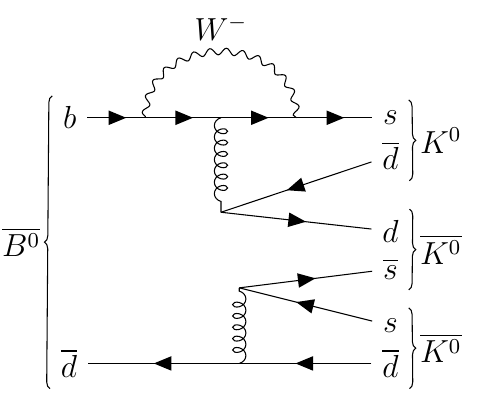
\includegraphics[height=4cm]{feynman3Ks01} 
\label{fig:side:a} 
\end{minipage}%
\begin{minipage}[t]{0.33\linewidth} 
\centering 
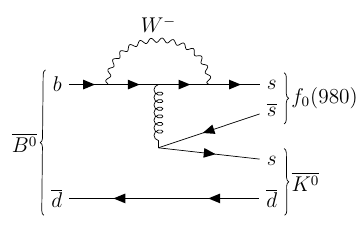
\includegraphics[height=4cm]{feynman3Ks02} 
%\caption{ } 
\label{fig:side:b} 
\end{minipage}% 
\begin{minipage}[t]{0.33\linewidth} 
\centering 
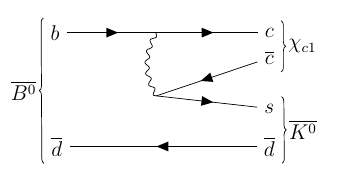
\includegraphics[height=3cm]{feynman3Ks03} 
%\caption{ } 
\label{fig:side:a} 
\end{minipage} %
\caption{non-resonant signal (left),resonant signal (middle) and tree-level resonant backgrounds (right)
$B^0_d\to3K^0_S$ diagrams}.
\end{figure}
\end{comment}



\begin{comment}
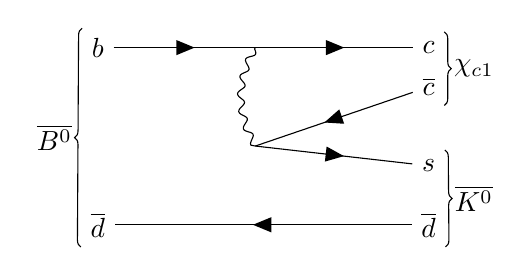
\begin{tikzpicture}
\begin{feynman}
\vertex (a1) {\( b\)};
%\vertex[right=1cm of a1] (a2);
\vertex[right=2cm of a1] (a3);
%\vertex[right=1cm of a3] (a4) ;
\vertex[right=2cm of a3] (a5) {\(c\)};
\vertex[below=1.25cm of a3] (a6) ;
\vertex[below=0.5cm of a5] (a7) {\(\overline{c}\)};
\vertex[below=1.5cm of a5] (a8) {\(s\)};
\vertex [below=0.75cm of a8] (b1) {\(\overline{d}\)};
%\vertex [left=2cm of b1] (b2);
\vertex [left=4.2cm of b1] (b3) {\(\overline{d}\)};
%\vertex [above=1cm of b2] (b4);
%\vertex [above=0.5cm of b1] (b5) {\({s}\)};
%\vertex [above=1.25cm of b1] (b6) {\(\overline{s}\)};
\diagram*{
{[edge=fermion],
(a1)--(a3)--(a5),
(b1)--(b3),
(a7)--(a6)--(a8),
%(b5)--(b4)--(b6),
},
%(b2)--[gluon] (b4),
(a3)--[photon, bend right] (a6),
%(a2)--[boson, half left,edge label=\(W^{-}\)] (a4)
};
\draw [decoration={brace}, decorate] (b3.south west) -- (a1.north west)
node [pos=0.5, left] {\(\overline{B^{0}}\)};
\draw [decoration={brace}, decorate]  (a8.north east)--(b1.south east) node [pos=0.5, right] {\(\overline{K^{0}}\)};
\draw [decoration={brace}, decorate]  (a5.north east)--(a7.south east) 
node [pos=0.5, right] {\(\chi_{c1}\)};
%\draw [decoration={brace}, decorate]  (a8.north east)--(b6.south east) 
%node [pos=0.5, right] {\(\overline{K^{0}}\)};
\end{feynman}
\end{tikzpicture}
\end{comment}

\chapter{Belle II experiment}
\section{Belle II and SuperKEKB overview}
The goal of the Belle II experiment is to search for evidence of New Physics, and the expected operation period is from 2019 to the end of 2030. The facilities are located in KEK, Tsukuba City, around 70 km in the north of Tokyo, Japan. The SuperKEKB accelerator enables electron-positron collision at the center-of-mass energy on the region of $\Upsilon(4S)$ resonances which is just above the mass of two $B$ mesons. The electron and positron beams are designed at 7 GeV and 4 GeV, respectively, with boost factor of 0.28, providing an environment for measuring time-dependent $CP$ violation by displacing the decay vertices of a $B$ meson pair in a measurable distance along the boosted direction. The SuperKEKB has a targeted luminosity of $8\times 10^{35}\: \text{cm}^{-2} \text{s}^{-1}$, a factor of 40 times higher than its predecessor, the KEKB.  Some key parameters of the SuperKEKB are listed in Table \ref{tab:superkekb_pars}. The schematic view of SuperKEKB and Belle II are shown in Figure \ref{fig:superkekb_belle2}.

\begin{figure}
	\centering 
	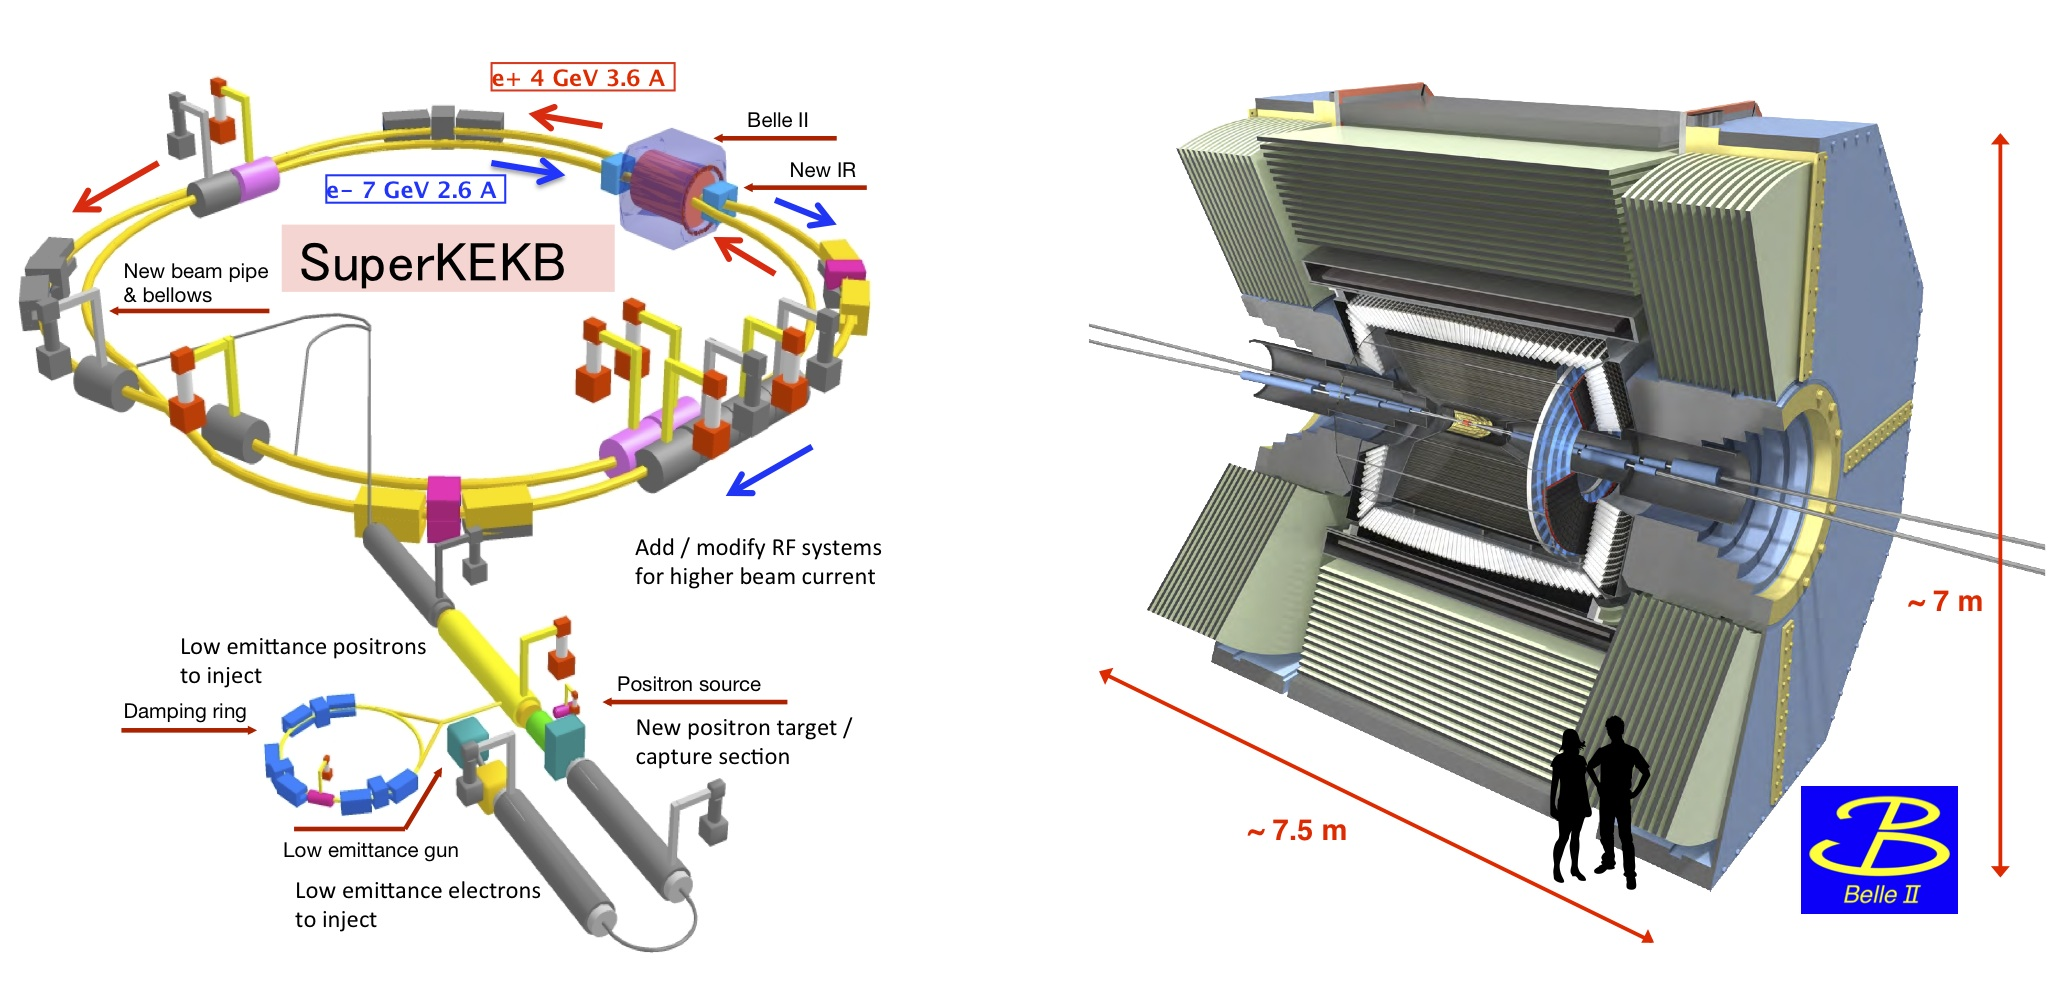
\includegraphics[height=7cm]{SuperKEKB-BelleII.jpg}
	\caption{The schematic view of SuperKEKB and Belle II detector \cite{Abe:2010gxa}.}
	\label{fig:superkekb_belle2}
\end{figure}

\begin{table}[H]
	\centering
	\large
	\caption{SuperKEKB parameters for low energy (LER) and high energy (HER) rings\cite{b2book}.}
	\label{tab:superkekb_pars}
	\begin{tabular}{c c c c}
		\toprule
		
		Parameters & LER ($e^+$) & HER ($e^-$) & Unit\\
		\hline
		Energy & 4.0 & 7.0 & GeV\\
		Half crossing angle & \multicolumn{2}{c}{41.5} & mrad\\
		Horizontal emittance & 3.2 & 4.6 & nm \\
		Emittance ratio & 0.27 & 0.25 & \%\\
		Beta functions at IP ($x$/$y$) & 32/0.27 & 25/0.30 & mm\\
		Beam currents & 3.6 & 2.6 &  A \\
		Beam–beam parameter & 0.0881 & 0.0807 & {}\\
		Luminosity & \multicolumn{2}{c}{$8\times 10^{35}$} &  $\text{cm}^{-2} \text{s}^{-1}$\\
		Perimeter of ring & \multicolumn{2}{c}{3} & km\\
		
		\bottomrule
	\end{tabular}
\end{table}


The Belle II detector has a close size as the Belle detector so that it is placed in the same shell, but all sub-detectors and electronic systems have been either newly built or considerably upgraded. The advantage of the SuperKEKB requires that the Belle II has to be able to stably operate at a 40 times higher event rates as well as 10 to 20 times higher beam background compared to Belle. The mitigation of the effects caused by such high beam background is essential to the success of the Belle II. Higher background level leads to higher occupancy and radiation damage to the detectors, along with more fake hits in the vertex detectors and central drift chamber, pile-up backgrounds in electromagnetic calorimeter and neutron-induced hits in muon detector. Data-acquisition system (DAQ) and trigger are also upgraded not only to adapt to higher luminosity but also for a better low-multiplicity event sensitivity. The Belle II detector in the top view is shown in Figure \ref{fig:belle2_view}.

\begin{comment}
 and expected performances are summarized as follows: 


\textbullet \space vertex resolution of $B$ mesons of $\sim 50 \: \mu\text{m}$,

\textbullet \space excellent reconstruction efficiency for charged tracks down to several 100 MeV and fairly good efficiency for charged tracks down to $\sim$ 50 MeV,

\textbullet \space excellent momentum resolution up to 8 GeV/c,

\textbullet \space highly efficient particle identification to separate $\pi^{\pm}$, $\mu^{\pm}$, $e^{\pm}$, $K^{\pm}$ and $p$ at full energy range of experiment,

\textbullet \space full cover of experimental acceptance solid angle,

\textbullet \space ultra fast and highly efficiency DAQ and trigger system to cope with large data quantities and fast triggering frequency. 
\end{comment}

\begin{figure}[htbp]
	\centering 
	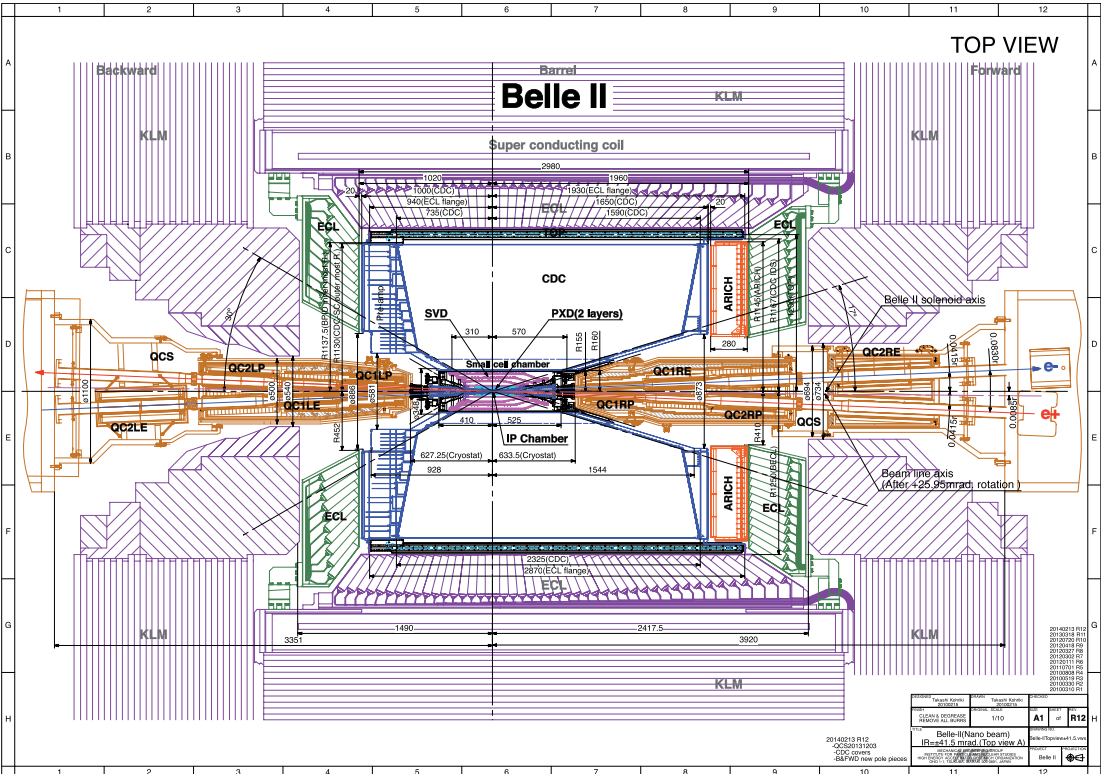
\includegraphics[height=10cm]{Belle2TopView.png}
	\caption{The Belle II detector top view \cite{b2book}.}
	\label{fig:belle2_view}
\end{figure}

The success of the Belle II detector depends on the complex of sub-detectors where each of them is design for specific purposes. The critical components and features are explained in the following sections. 

\section{Vertex detector (VXD)}
The vertex detector is composed of two detectors, the silicon based pixel detector (PXD) and silicon based vertex detector (SVD), where total 6 layers are placed in the inner-most region from interaction point (IP).  The geometry of VXD is shown in Figure \ref{fig:svdgeo}. The PXD is placed at a radii of $r=14$ mm and $r=22$ mm with DEPFET\cite{Abe:2010gxa} type pixel sensors, which is designed to provide two dimensional hit position information. The inner layer leaves a sufficient space for possible variations of the beampipe layout. The size of two layers are determined by the required acceptance angle, which is 17 degrees (forward) to 150 degrees (backward). The pixel sensor is a monolithic structure with current-digitizing electronics at the end of the senor which makes a very thin  layer at about 50 microns. The schematic view of sensors on PXD is shown in Figure \ref{fig:pxd}.
\begin{figure}[htpb]
	\centering
	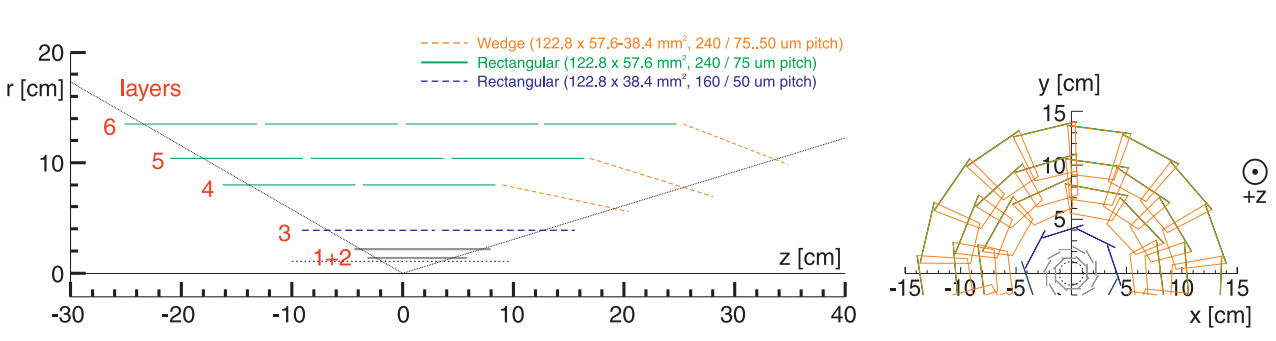
\includegraphics[height=5cm, width=1\linewidth]{VXDGEO.png}
	\caption{A schematic view of of PXD and SVD. Two PXD layers are in grey, SVD layer 3 is in blue and layer 4, 5, 6 are in green\cite{Abe:2010gxa}.}
	\label{fig:svdgeo}
\end{figure}
\begin{figure}[htpb]
\centering
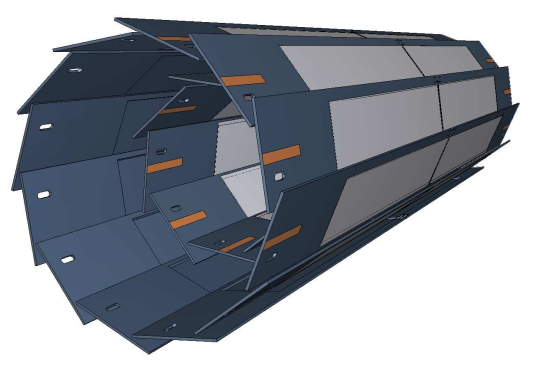
\includegraphics[width=0.6\linewidth]{pxd}
\caption{The geometry of sensors on PXD where the light grey surfaces are DEPFET sensors with a thinness of 50 microns. The full length including the out modules is 174 mm \cite{Abe:2010gxa}. }
\label{fig:pxd}
\end{figure}
 As the very close range the PXD is, the sensors are exposed to a very high event rate and very high beam background environment. The large data flow from PXD without any data reduction scheme is problematic for data acquisition system. In order to reduce the data that is not interested by physics analysis such as beam backgrounds, a fast online tracking system is built up for searching a ``region of interest" (ROI) on the PXD sensors. To be specific, the data from PXD will be first readout to a system called ``ONSEN" which can store large size temporary data up to 5 seconds. In this timing window, a fast online tracking system will perform a track fitting using vertext detector and central drift chamber to extrapolate the fitted tracks backward to PXD plane so the ROI on the PXD sensors can be defined. The data from PXD outside of the ROI is not read out to external tapes where offline data is written. 

SVD detector consists of 4 layers of detectors called  ``double-sided silicon strip detectors" (DSSDs) at 39 mm, 80 mm, 104 mm, and 135 mm away from IP, respectively. The two sides of the sensors are called $p$-side and $n$-side, where the former is for strips on $r-\phi$ direction (transverse direction) and the latter is for strips on the $z$ direction (beamline direction). To suppress the background hits, a readout chip with a fast shaping time of $\mathcal{O}$(50 ns) is indispensable. The APV25 chip \cite{french2001design} is chosen as the readout chip that was originally developed for CMS silicon tracker, with total 128 identical channels of low-noise preamplifiers followed by a 50 ns peaking time shaper stage. The polar angular acceptance ranges from 17 degrees to 150 degrees, which is asymmetric to account for the
forward boost of the center-of-mass frame. The combination between sensors, electronics and the supporting structure uses so-called ``Origami" concept which stands for a chip-on-sensor design, as shown in Figure \ref{fig:origami}. In the Origami scheme, the readout chips APV25 are placed on a single flexible circuit mounted on the $n$-side of the sensors. The channels of $p$-side are attached by small flexible fan-outs wrapped around the edge of the sensors. All connections between flex pieces, sensor, and APV25 chips are made by wire bonds.
\begin{figure}[htpb]
	\centering
	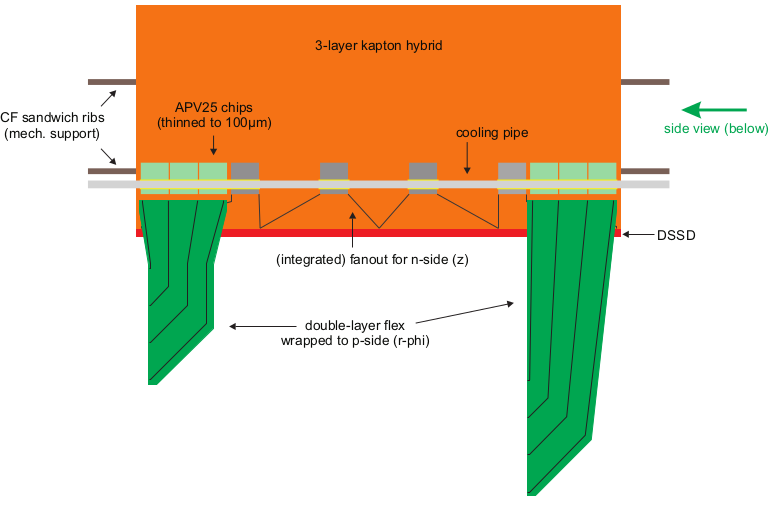
\includegraphics[width=1\linewidth]{ori1}
	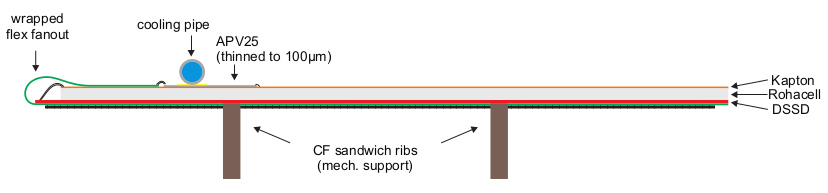
\includegraphics[width=1\linewidth]{ori2}
	\caption{The top and side views of Origami chip-on-sensor design for DSSDs of SVD. Top: the APV25 chips in grep read out the same side sensors channel while chips in green read out the sensors on the opposite side using wrapped-around flex pieces. Bottom: side view of the Origami design shows the location of wrapped flex which connects the strips of the bottom sides which are placed at the left edge.\cite{Abe:2010gxa}}
	\label{fig:origami}
\end{figure}



\section{Central drift chamber (CDC)}
The central drift chamber (CDC) is the core component of spectrometer in the Belle II, which consists of a fairly big drift chamber made of many small drift cells filled with gas. The chamber
gas is comprised of a He–C$_2$H$_6$ 50\%:50\% mixture with an average drift velocity of 3.3 cm $\mu$s$^{-1}$ and a
maximum drift time of about 350 ns for a 17 mm cell size.
The out radius of CDC has been extended to 1130 mm from 880 mm of Belle, owed to a new thinner particle identification detector which will be introduced in the next section. The whole CDC contains 14336 sense wires in 56 layers, placed in the axial direction and the stereo direction\cite{b2book}\cite{Abe:2010gxa}. Such a design can utilize the information from axial and stereo wires to construct a full 3 dimensional hits which reflects helix tracks in CDC volume. Thus, CDC is one of the key components for measuring the helix parameters for tracking, providing precise information on the charged tracks momentum. Also, it provides particle identification information using measurements of energy loss within its gas volume. Low-momentum tracks, which do not reach the particle identification device, can be identified using the CDC alone. Finally, it provides efficient and reliable trigger signals for charged particles.

The Belle II CDC is expected to handle higher trigger rates with less dead time. The front-end electronics are located near the backward end-plate and send digital signals to the
electronics hut through optical fibers. Due to the higher radiation and higher beam background in the Belle II, also to create more space for SVD volume, the inner radius of CDC in Belle II is 160 mm. CDC can also create three dimensional trigger information from a dedicated trigger type called $z$ trigger\cite{Abe:2010gxa} based on the 3D tracking achieved by an FPGA using axial and stereo wires.

The structure of CDC consists of three main components which are a thin carbon-fiber reinforced
plastic (CFRP) inner cylinder, two aluminum endplates, and a CFRP outer cylinder, as shown in Figure \ref{fig:cdc_full}. The outer cylinder is a thickness of 5 mm structure supporting most of the wire tension of 4 tonnes. The inner cylinder is as thin as 0.5 mm to minimize the material and support small cell chamber such as the layers in the inner most region. 

\begin{figure}[htpb]
	\centering
	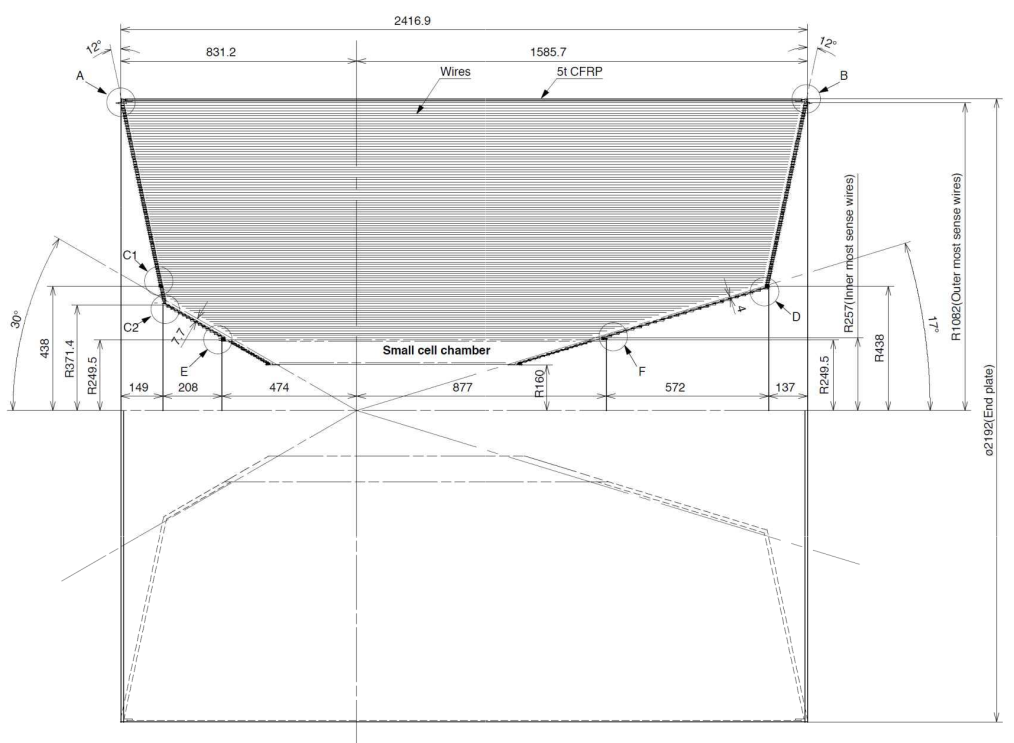
\includegraphics[width=1\linewidth]{cdc_full}
	\caption{CDC structure schematic view \cite{Abe:2010gxa}.}
	\label{fig:cdc_full}
\end{figure}





\section{TOP and ARICH detectors}
The particle identification (PID) system of the Belle II mainly consists of two parts, time-of-propagation counter (TOP) and aerogal based Cherenkov radiation imaging ring (ARICH).

TOP is the specialized detector that can reconstruct Cherenkov radiation's time of arrival and generated position by a photon detector placed at the end of a 2.6 cm quartz bar. The TOP is placed at the barrel region of the spectrometer, as shown in Figure \ref{fig:belle2_view}. The conceptional view and the working principle of TOP counter are shown in Figure \ref{fig:top}. In this counter, the time of propagation of the Cherenkov photons that are internally
reflected inside a quartz radiator is measured. The quartz radiator is composed of three components. The first is a long bar for radiating Cherenkov photons. The photons then propagate via total internal reflection towards the bar end, where the MCP-PMTs are mounted. The second is a spherical mirror installed on the forward end of the bar for focusing the photons. The third is a prism that attaches to the backward end of the bar which allows the Cherenkov ring image to expand before the photons are recorded by the PMTs. By this structure, a 3-dimentional information with $x-y$ position and a timing information are obtained by micro-channel plate (MCP) PMTs at the end surfaces of the quartz bar.
The resolution of starting time is achieved about 50 ps \cite{Abe:2010gxa}. As the key component of the photon detector, the squared shape MCP PMTs, donated as SL-10 \cite{inami2008cross}, have been developed with a $4\times 4$ anode array, a multi-alkali photocathode,
two MCP plates with 10 $\mu$m pore size, and an aluminum layer on the second MCP to protect
against ion feedback. The image of a SL-10 MCP PMT and an anode schematic view are shown in Figure \ref{fig:mcppmt}. 

\begin{figure}[htpb]
	\centering
	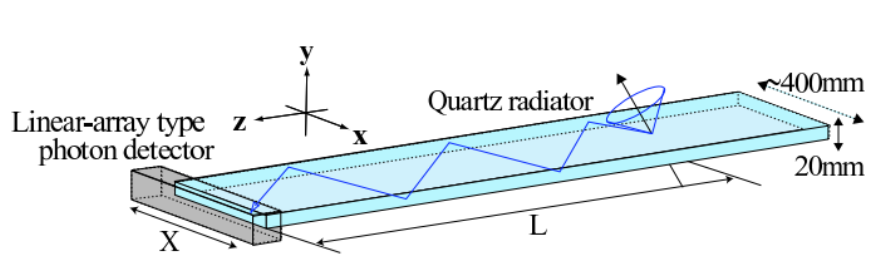
\includegraphics[width=0.7\linewidth]{top_mod}
	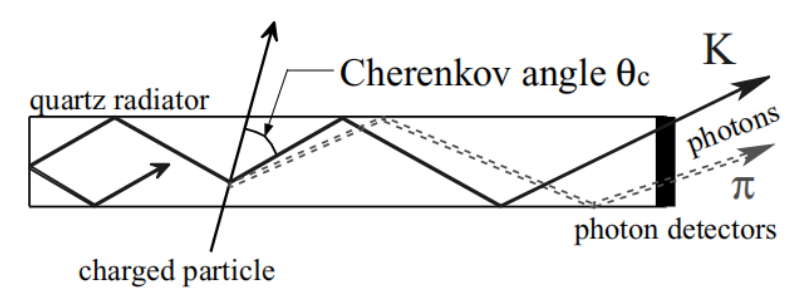
\includegraphics[width=0.7\linewidth]{top_img}
	\caption{Conceptional view of TOP counter (up) and its imaging process of $K^{\pm}$ and $\pi^{\pm}$ (down) \cite{Abe:2010gxa} for PID purpose.}
	\label{fig:top}
\end{figure}

\begin{figure}[htpb]
	\centering
	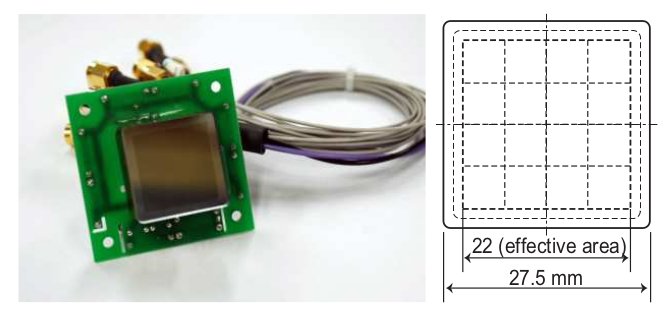
\includegraphics[width=0.8\linewidth]{mcppmt}
	\caption{SL-10 MCP PMT (left) and the schematic view of $4\times 4$ anode (right) \cite{Abe:2010gxa}}
	\label{fig:mcppmt}
\end{figure}

Aerogel Ring-Imaging Cherenkov
detector (ARICH) is located at the forward endcap in Figure \ref{fig:belle2_view} to separate charged particles in a momentum range from 0.5 GeV/c to 4 GeV/c, which requires single-photon-sensitive high-granularity sensor to reconstruct the Cherenkov angle with small photon yield.  
Hamamatsu company and the hardware experts from the Belle II collaboration have developed a hybrid avalanche photon detector (HAPD) to meet the requirements. Each sensor is $73 \times 73$ mm$^2$ embedded with 144 channels to accelerate emitted electrons in a 8 kV field. Avalanche photo-diodes (APD) are used for the detection of electrons at the end of electron acceleration, see Figure \ref{fig:arich_img}. The ARICH detector outlook and the ring image of cosmic muon on the HAPD sensors are shown in Figure \ref{fig:HAPD}.

\begin{figure}[htpb]
	\centering
	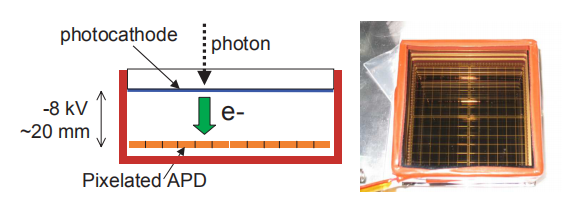
\includegraphics[height=5cm]{HAPD}
	\caption{Photon-electrons acceleration (left) and pixelated APD (right) at the end \cite{Abe:2010gxa}.}
	\label{fig:arich_img}
\end{figure}



\begin{figure}[htpb]
	\centering
	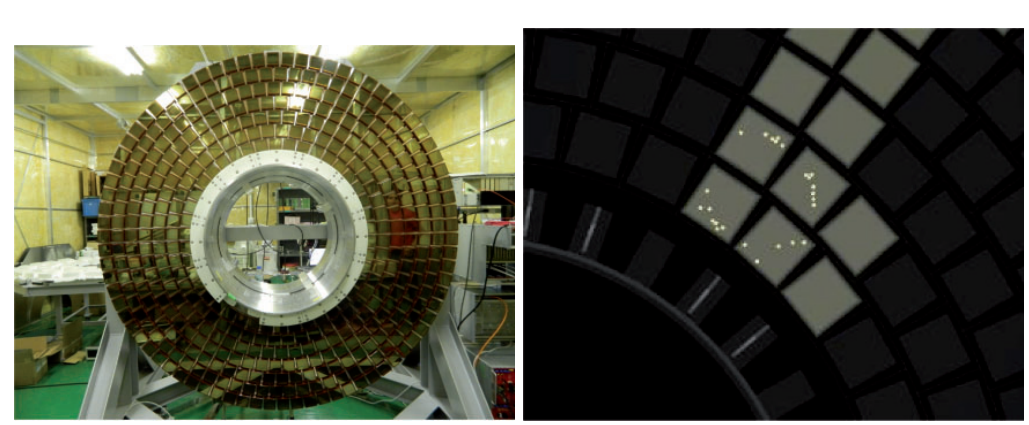
\includegraphics[height=6cm]{ARICH}
	\caption{ARICH detector (left) and the ring image of cosmic muon on the HAPD sensors\cite{b2book}.}
	\label{fig:HAPD}
\end{figure}

\section{Electromagnetic calorimeter (ECL)}
The electromagnetic calorimeter (ECL) in the Belle II is mainly responsible for the detection of $\gamma$ radiation and electrons, providing energy deposition information for trigger, particle reconstruction and PID. ECL consists of three sections as shown in Figure \ref{fig:belle2_view}: a 3 m long barrel section with an inner radius 1.25 m, and two annular endcaps at $z = 1.96$ m (forward) and $z = -1.02$ m (backward) from the IP. The barrel section contains 6624 CsI(TI) crystals of 29 distinct shapes and each crystal is a pyramid shape with about $6\times 6$ in cross section and 30 cm in length. The endcaps section contains 2112 CsI crystals of 69 shapes and the total number of crystals is 8736, with a total
mass of about 43 tons \cite{Abe:2010gxa}.

As the basic component of ECL, the  thallium doped caesium iodide CsI(TI) crystals are assembled tightly in end-caps and barrel sections. Compared to the previous ECL in Belle, the pre-amplifiers and the structures remain unchanged, while the readout  electronics have been upgraded. The estimated background level in Belle II ECL will cause the much longer decay time in the scintillation of CsI(TI). This will lead to the pile-up effect of readout noise. To compensate this effect, wave-form sampling electronics are embedded with the photon detectors (PMT).
 
\begin{comment}
Especially in the forward direction of the electron beamline, where the level of beam background is much higher, the effect of pile-up noise becomes even worse and the performance of ECL will be of trouble if no special measure taken. Therefore, the pure CsI crystal is considered to be chosen as the material of detector to achieve a fast wave-shaping time and higher radiation tolerance compared to the dosed CsI(TI), which is an back-up option for the future upgrade. ECL is the most important detector for providing trigger information for low multiplicity events, since the main feature of these events is one or two energetic photon(s) emitted from IP region while the charged tracks are missing. 
\end{comment}
  

\section{$K_L^0$ muon detector (KLM)}
The $K_L^0$ and muon detector (KLM) system of the Belle II consists of a sandwich stacked iron plates at outside of the superconducting solenoid and it acts as a return york of the magnet. The iron plates serve as the interaction materials with $>$ 3.9 times the interacting length of material ($\sim 132.1$ g/cm$^{2}$) compared to the ECL, allowing $K_L^0$ particles to shower through. The octagonal barrel covers the polar angle range from 45 degrees to 125 degrees, while the endcaps extend
this coverage from 20 degrees to 155 degrees. There are 15 detector layers and 14 iron plates in the barrel and
14 detector layers and 14 iron plates in each endcap. The side view of KLM is shown in Figure \ref{fig:klm}.
The Belle KLM material uses the glass-electrode resistivity plate chambers (RPC) which is not suitable for the Belle II due to high background level.  Neutrons dose is significantly larger due to the much more electromagnetic radiation reaction on detector materials. The long dead time of RPC under such dose rate will reduce the efficiency of KLM. To mitigate this problem, the RPCs are replaced by the layers of scintillator strips with wavelength-shifting fibers, read out by silicon photomultipliers (called ``SiPMs", Geiger mode operated APDs) as light sensors, which is proven to be able to reliably operate by setting up the discrimination threshold \cite{b2book}.

\begin{figure}[htbp]
	\centering
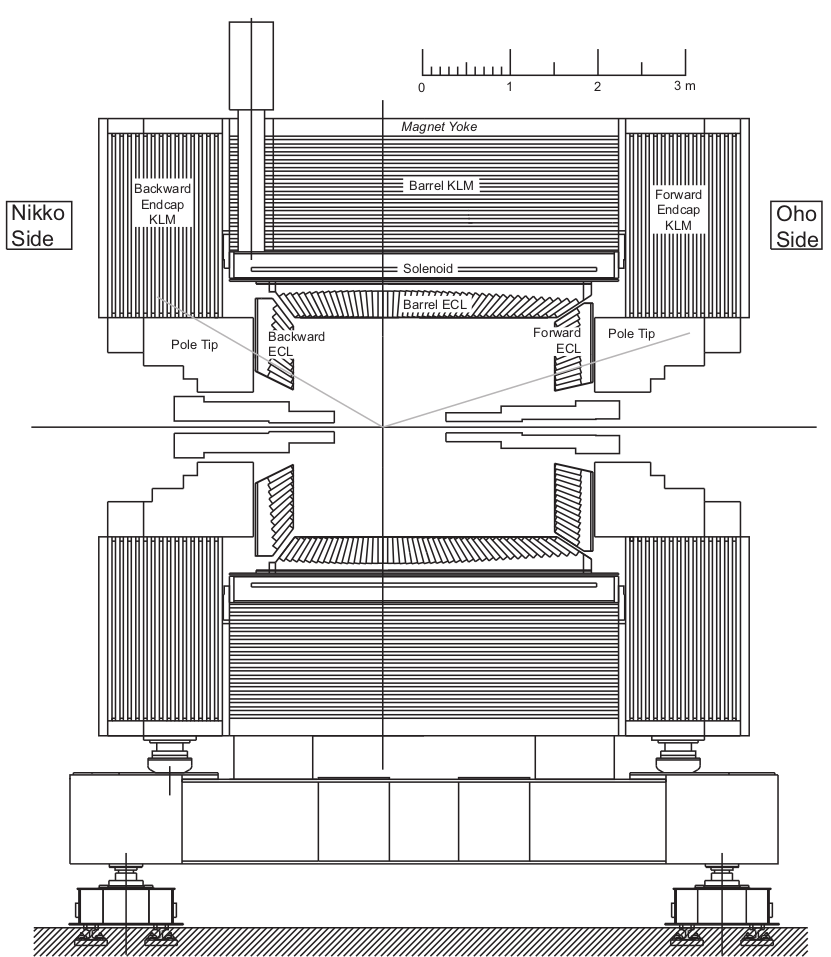
\includegraphics[width=1\linewidth]{klm}
\caption{The side view of KLM in between the ECL and the solenoid, which the grey lines presents the nominal acceptance angle of the Belle II \cite{Abe:2010gxa}. }
\label{fig:klm}
\end{figure}




\section{Trigger and DAQ system}
The interesting topics in Belle II physics analysis highly depend on the trigger system. The Belle II trigger system is composed of two levels: a hardware-based, low-level trigger called ``L1" trigger, and a software-based high-level trigger (HLT). The L1 trigger has a latency of $\sim 5 \-\mu\text{s}$ and the maximum trigger output rate is 30 kHz, which is limited by the read-in rate of data acquisition system (DAQ). Considered the high event rate and background level from future Belle II luminosity, a series of upgrades have been implemented for L1 trigger. The key improvements of L1 come from the firmware-based reconstruction algorithm and trigger logic.

The HLT, as the second level of Belle II trigger systema, plays an important role in DAQ. As discussed in the section of PXD, the data size in PXD is huge at high luminosity and the ROI selection must be applied to reduce it. The HLT will first use fast online tracking by CDC and ECL information to further reject the residual beam background not found by L1 trigger. Only the events passing this step are considered for the full event reconstruction. Then the information from all detectors except for PXD are fed into the first event builder for full event reconstruction. The event rate is reduced to about $6$ kHz by HLT which uses the full reconstruction information to find track-associated hits on PXD, as introduced as ROI before. The workflow of DAQ with HLT is demonstrated in Figure \ref{fig:daq}. The reduced event rate by applying ROI finding on PXD and other detector read-out systems are combined into the second event builder and eventually written to the offline storage. 

\begin{figure}[htbp]
	\centering
	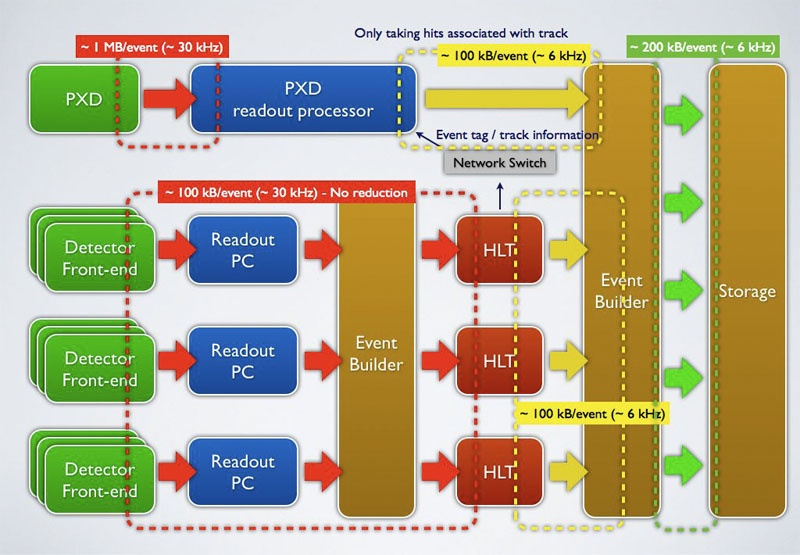
\includegraphics[width=0.8\linewidth]{Belle2DAQ}
	\caption{The Belle II DAQ workflow with HLT between two event builder to reduce the original 30 kHz event rate down to about 6 kHz for offline storage.}
	\label{fig:daq}
\end{figure}


%2021/02/16 ends
Since the primary goal of the Belle II is focusing on $B$ physics studies, it is natural that the trigger system should be able to operate over all of the interesting $B$ physics conditions, with normally 3 or more CDC tracks and large energy deposition in ECL. By studying the efficiency using the simulated events, close to 100\% $B$ decays are recorded by Belle II trigger system. Besides, the Belle II detector is expected to capture many other physics events such as searching for leptonic flavor violation using $\tau$ decays or dark matter particles, of which the performance is highly affected by the beam background level and trigger efficiency. Therefore, the control of beam background becomes essential, which mainly consists of beam-gas scattering, synchrotron radiation, the radioactive Bhabha scattering, the two-photon process, beam-beam effects, and Touschek effect. Their impacts depend on many factors such as beam current, luminosity and vacuum conditions, etc. One of the featured topology of these beam background events is the combination of two charged tracks in CDC and one or two clusters in ECL. The sources of the main beam backgrounds and their event rates in simulation are listed in Table \ref{tab:BG}.

\begin{table}[htbp]
	\centering
	\large
	\caption{Simulated beam background rate \cite{b2book}}
	\label{tab:BG}
	\begin{tabular}{c c c}
		\toprule
		Type & Source & Rate (MHz)\\
		\hline
		Radiative Bhabha & HER &  1320\\
		Radiative Bhabha & LER &  1294\\
		Radiative Bhabha(wide angle) & HER &  40\\
		Radiative Bhabha (wide angle) & LER &  85\\
		Touschek scattering & HER &  31\\
		Touschek scattering & LER &  83\\
		Beam–gas interactions & HER &  1\\
		Beam–gas interactions & LER &  156\\
		Two-photon QED & - & 206\\
		\bottomrule
	\end{tabular}
\end{table}
\begin{comment}
The improvements on both L1, HLT and the DAQ system are dedicated to serve the operation of the Belle II detector with much higher event rate in future. The further upgrades are also considered such as the replacement of the current DAQ module (COPPER board\cite{Abe:2010gxa} on the read-out PCs) with the latest PCIe-40 platform\cite{mitra2016gbt} to enlarge the bandwidth between detector front-end electronics and the event builder in Figure \ref{fig:daq}.
\end{comment}



\begin{comment}
Based on the reasons discussed above, Belle II trigger has been designed to have 2 separated levels of triggers. Low level trigger, also called as L1 trigger, is hardware-based trigger. and high level trigger (HLT) is the software based trigger.
The L1 trigger rate can go up to 30kHz that is also the up-limit of DAQ read-in rate. The latency of L1 is control to be 5 $\mu$s, improved from Belle trigger.
And yet 30kHz is still to high for writing out the data to tape, so the HLT must be implemented to reduce the trigger rate to about 10kHz and it has to be able to select ROI on the PXD to reduce the data flux limited by bandwidth of read-out cables. To do that, HLT utilize  the full offline reconstruction algorithms to allow the access of full-granularity
event reconstruction using all detectors except for the PXD. 

\end{comment}

%2021.01.27 ends here
\begin{comment}
\section{Detector simulation}
The Belle II simulation makes a use of GEANT4 software. GEANT4 package can accept the event created by module called ``particle gun" which directly injects particles to detector volume. Or it takes in software simulated data, which in general is called ``event generator". Belle II Analysis Framework (BASF2) software (see the next section for the details of BASF2) provides the interface for createing simulated data from event generator to GEANT4. Most of the primary particles are simulated by event generator and sent to GEANT4 for simulation between detectors' components. The out-flying particles that has relatively long life time compared to the primary interaction such as $K_S^0 \to \pi^+ \pi^-$ are simulated in GEANT4 after the event generator does its job. Exchanged bosons and primary electrons(positrons) will not be feed into GEANT4. Then GEANT4 creates secondary particles during the particle interaction and detector material, such as the radiations from charged tracks and also the scattering processes with detector materials. The hits digitization are generated by other BASF2 modules using primary and secondary particles together. Finally, the response from detectors are sent to the persistent data storage (called ``DataStore" as C++ objects, detail in next section.) to be used in the analysis chain of BASF2. 

For each type of the particles and each type of detector material, the interaction is varied in different processes. The co-responding process of physics should be specified by the users or using the provided list from GEANT4 developer group. In Belle II simulation, the
Fritiof quark–gluon string model at high energy and the Bertini intra-nuclear cascade model at low
energy are used by default from GEANT4 list. 

The simulation of the beam background is done by a software called SAD, as external part of BASF2. It simulates the flux of particles from the beamline of the SuperKEKB accelerator. Whenever a particle trajectory deviates from the beamline region and hit the Belle II detector part, its momentum and position vectors will be saved into a configuration file. Then such configuration file will provide the initial information for GEANT4 simulation software to simulate the interaction between the given particle and Belle II detector, which is eventually analyzed as normal particles by BASF2.
The output of BASF2 is standard ROOT format and it presents how a beam induced particle interacts with detector material to create simulated hits as beam backgrounds. 

The mixing of background is then implemented to provide a realistic view of physical events and beam background overlay. Since the format of beam background is simulated hits, thus adding the background events is done by injecting the simulated hits, then move to the digitization of hits to detector responses. In a event time window $\Delta t$, assuming the given type background has a average rate of $R$, the mixing number of background hits in such event is: 

\begin{equation}
\bar{N} = sR\Delta{t}
\end{equation}

$s$ is optional scaling factor which can be used to study the influence of given type background in different level. Because $R$ is averaged value, in the actual mixing, the number of $\bar{N}$ is used as the expected value of Poisson distribution, which presents the number of observed events when many trials of such events is made with certain small possibility per event.  In order to simulate the effect of timing different of background and physical events, the mixing timing window over $\Delta t$ is randomly shift according to the physical events.
With the real experimental data comes in handy, the method of adding background events to physics events is slightly different since using real beam background can provide a more precise result than simulation. By setting a random trigger for beam background, the hits digitization from real beam background will be collected and add to simulated physics events. Although the pile-up noise collected in this method is not very precise because of the threshold set for detectors allowing only part of noise to be added, the non-recorded noise can still contribute to the pile-up noise for physics events, and they are not included in this method. Yet overall it provides a more realistic evaluation of beam background overlay.

\end{comment}

\section{Analysis software framework} 
The data acquired by the Belle II experiment or simulation can be processed by the Belle II Analysis Software Framework, called BASF2. It has a good capability to handle multiple tasks for the Belle II data analysis, from the simulated data production to physics events reconstruction. The BASF2 takes the advantage of good efficiency and reliability of C++ as the programming languages, but the use of
Python is also allowed when it shows clear advantages, such as steering the analysis workflow. 

 %The official BASF2 is developed in different release versions, light-versions and featured-versions. In this thesis, release-05-01-01 version is used. 

\subsection{BASF2 Core Structure}
The core structure of BASF2 contains three major parts: the analysis packages required by the needs of analyzing the Belle II data such as finding tracks and combining particles, the external libraries as the third-party software such as ROOT\cite{ROOTcern}, and the tools for configuring and installing BASF2 which are mostly Python and shell scripts. Data analysis is supported by providing
a series of modules belonged to BASF2 for appropriate reconstruction based on their specific
needs. To realize this, a modular analysis workflow, where each module can handle the event
data through an unified method such as ROOT I/O based object persistency, is desired. Other
processes, such as data summary table (DST) processing, simulation of each sub-detectors, and data skimming, are done with the packages built for sub-detectors.

The packages are categorized based on the different levels of Belle II detector components, like the packages of base-level system control called ``framework", the package that provides the simulation of each sub-detectors like ``svd",  the package for track reconstruction called ``tracking",  and the package for post-reconstruction data analysis called ``analysis", etc. Users can work either with compiled binary version of BASF2 installed centrally on working servers, or build from the source based on their own need. Furthermore, the distributed computing is also supported by the installations of BASF2 through the managment service provided by DIRAC system \cite{dirac}. The detail information about the core structure of BASF2 can be found in Ref.$\sim$\cite{kuhr2019belle}. 




\begin{comment}
As for the externals, it contains the many packages or libraries that provide functionalities BASF2 needs during the execution or installation. For example, some basic packages, like gcc compiler, cmake, tar, wget, Python and git are included. In particular, due to the dependence of the analysis tools that may be frequently used by Python, around 100 additional Python packages are installed as the externals, such as ``Numpy" and ``matplotlib" packages that provide functions for statistical calculations and plotting. The complexity of building all of these external software could be tough for users so that the compiled versions that cover the common platforms are available from BASF2 official repository. 
Tools are collections of shell or Python scripts for setting up BASF2 and externals environment. It can easily handle the need of setting up an environment of specific BASF2 version and the externals tied to that version. It also provides a function to setting up the environment of developing BASF2, where developers can get one developing copy of BASF2 and write the additional codes as the modification, so the compatibility of BASF2 could be easily maintained by building a release version from the developing branches. In this thesis, two new packages are developed and built with release-05-01-01 version BASF2. This developing version of BASF2 contains all functions that release-05-01-01 has. The details will be discussed later. 
\end{comment}

\subsection{Event processing workflow}
The data from Belle II detector or from the simulation, are organized into a set of runs that are defined by either experimental conditions or simulation conditions. For instance, the simulation data from the condition of a certain detector is packed together, marked with the condition database index used during the simulation.  Such data sample then is divided into different runs based on estimated luminosity from experiment, which can contain the different number of events in each run.  This scheme is used for categorizing experimental data as well, so that users can easily know which experiment conditions are used. Thus, when BASF2 processes a data set, the functions are called for every event based on different configurations that are corresponding to the different experiment conditions. For example, in a data set where events are recorded with the different magnetic fields, BASF2 can automatically change the configurations of the magnetic fields event-by-event to provide a better track measurement. Based on this idea, all BASF2 functions (called ``modules") are developed based on a python module class which contains following embedded functions to be called at event-based level: 


\textbullet \space initialize: called at the start of processing events to prepare this run, including how many events will be processed and declaration of the buffer space and memory required by this module.

\textbullet \space beginRun: called after the initialization is finished and before the event read-in starts, including setting up database conditions used in this run (run-dependent configurations) or event (event-based configurations).

\textbullet \space event: called when each event is read and start to process. This is the actual processing step, such as perform tracking or combining all daughters to find a mother particle. 

\textbullet \space endRun: called at the end of a run, usually to register all processed information to the storage, such as physics variables from all reconstructed particles.

\textbullet \space terminate: called at the end of the processing of all events, release the buffered space and memory.

BASF2 executes a series of modules loaded dynamically to process the data set for analysis purposes, which is shown as Figure \ref{fig:b2flow}. The selection, configuration and executed order of the modules are defined by a file called ``steering file" written in Python. The modules parameters are attributes which can be set during the runtime using the steering file. 
\begin{comment}
For example, the ``Path" object declared in a steering file stores the sequence of modules that will be executed, to which allow other modules such as ``mdstInput" or ``reconstructDecay" to be added.
Users can use ``boolean" type variable set in ``event" function to create a conditional branch of a ``Path" in case that one event needs to be processed with different modules at the same time. For instance, in the decay reconstruction package, if a decay chain is not fulfilled by missing one particle in the ``event" functions, other back-up decay chains can be checked to see if a successful reconstruction is possible.  
\end{comment}


\begin{figure}[htpb]
	\centering
	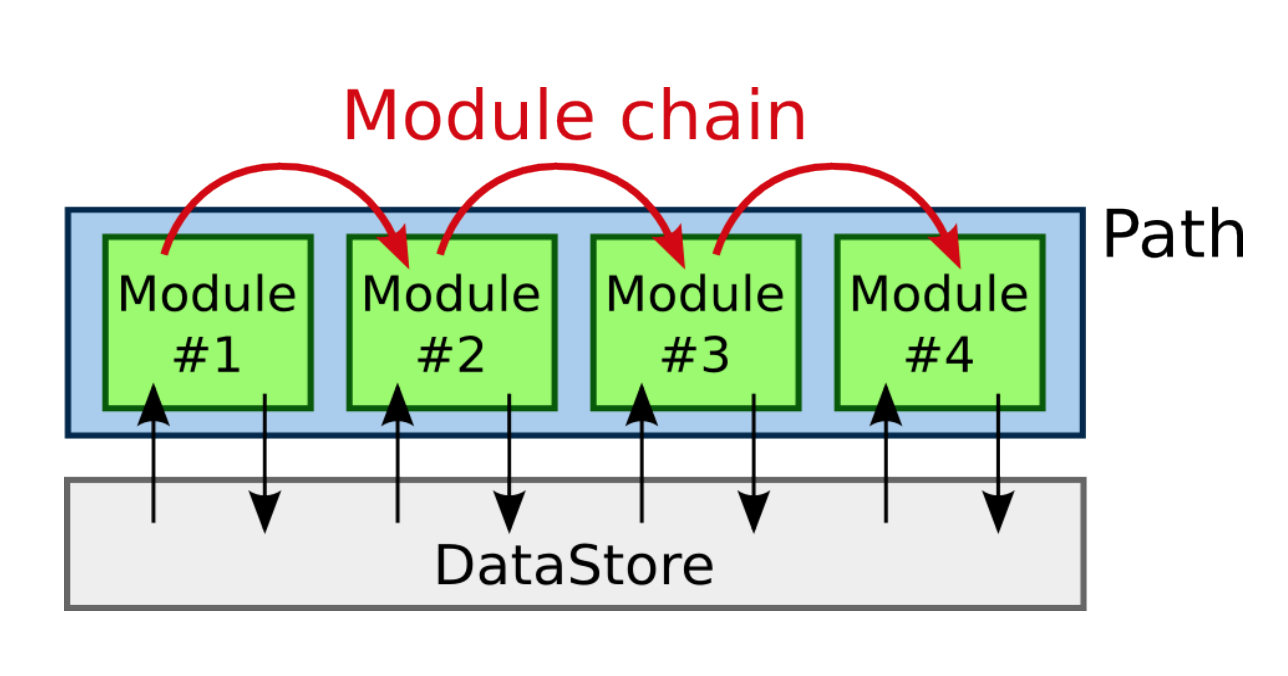
\includegraphics[width=0.8\linewidth]{b2flow}
	\caption{The module-based analysis workflow in BASF2.}
	\label{fig:b2flow}
\end{figure}

The object that interacts with BASF2 I/O is called ``DataStore", as shown in Figure \ref{fig:b2flow}. This implementation doesn't depend on the event data model. The only mandatory component is called ``EventMetaData" which presents the experiment, run  and event number of a event. ``Unpacker" module converts the raw digits into digits-based object in BASF2. In simulation, digitization is done by module called ``digitizer". The digits-based objects are further processed to form hits or clusters depending on detector types. Higher level functions such as tracking and decay reconstructions are implemented based on these basic information by their packages. Eventually, BASF2 writes out the information based on users' needs, like kinematics variables, to ROOT format files, or simply prints out processing statistics to the standard output. 

\begin{comment}
In practice, BASF2 starts running when it checks there is at least one module specifying the number of events to be processed in a ``path"  from the ``steering file", then it reads in the information from DataStore in the input ROOT file, execute all the requested modules in the ``steering file" and return the time and number of events as information printed in standard output.
\end{comment}



\subsection{mDST structure}

The output of BASF2 processing from the online data contains several detector-specific objects, which are restored as mini data summary table (mDST) type ROOT file. For a mDST level analysis, the goal is usually aimed to find particles from physics processes and reconstruct decay information. A output mDST ROOT file contains the reconstructed objects from each sub-detectors, and the following items are required for $B^0 \to K_S^0  K_S^0  K_S^0$ analysis. 


\textbullet \space Track: object presenting any charged particle trajectory. It's linked to multiple track fit results using different nominal mass hypotheses as well as their track fit quality to help select good tracks.  

\textbullet \space TrackFitResult: the fitting result of tracks with different mass hypotheses. It consists of five helix parameters, their covariance matrix and p-value from the fit. It also stores the information of hit pattern on VXD and CDC. 

\textbullet \space V0: object for the relative long-lived neutral particles that fly out of interaction region but mostly decay or interact inside detector region. In Belle II, these are mostly $K_S^0$, $\Lambda$ and photon converted to a electron-positron pair. V0 also stores their relation to the charged daughter tracks and track fit results for further selections.


\textbullet \space PIDLikelihood: it presents for the possiblity of a charged track to be an electron, muon, charged kaon and pion, proton and deuteron provided by particle identification system. 

\begin{comment}
\textbullet \space ECLCluster: reconstructed cluster in ECL detector. It consists of energy deposition and hit positions as well as other hit shape related variables. If a cluster is matched with an extrapolated track, a relation between them will also be created. 

\textbullet \space Reconstructed cluster KLM detector. It consists of momentum and position measurement. If a cluster is matched with an extrapolated track, a relation between them will also be created. 

\textbullet \space KLId: $K_L^0$ candidates with the particle identification as related to KLM and ECL clusters. 

\textbullet \space TRGSummary: L1 trigger information. 

\textbullet \space SoftwareTriggerResult: HLT information mapped by trigger names to trigger results. 
\end{comment}

\textbullet \space  MCParticle: simulated particles and particle-detectors relations are
created if simulated particles are correctly reconstructed as
tracks or clusters.
 

%2020.01.28 ends
\subsection{Conditional Database}

In addition to the physics data, analysis relies on various conditional data that are different calibration of detector, weight files for multi-variate analysis usage like PID and so on. This data is stored in a central database server called central Conditional Database\,(CDB)\,\cite{BASF2}. 
Conditions are made of payloads and each payload has its own``Intervals of Validity" (IoV) which defines in which runs the payload is valid. A collection of the payloads that are produced based on a certain stage of the experiment is packed together and called as a global tag (GT). 
\begin{comment}
A set of payloads and IoVs are called a global tag (GT). Considered the GT that is required by the different analysis purposes may change even though the experiment condition is still same, GT is subjected to be updated once new calibrations of detectors or weight files for analysis tools are available.
\end{comment}


\begin{comment}
On the users' side, except for just using central database, a local database back-end that takes GT information such as calibration data while uses a local database, such as a customized PID weight file,  is also possible.  It automatically download the needed database files that are required for a BASF2 execution and stores them in a local folder. This means even if the local machine is offline or the CDB is not accessible, one can still run BASF2 as long as the local folder is there. 
\begin{figure}[htbp]
\centering
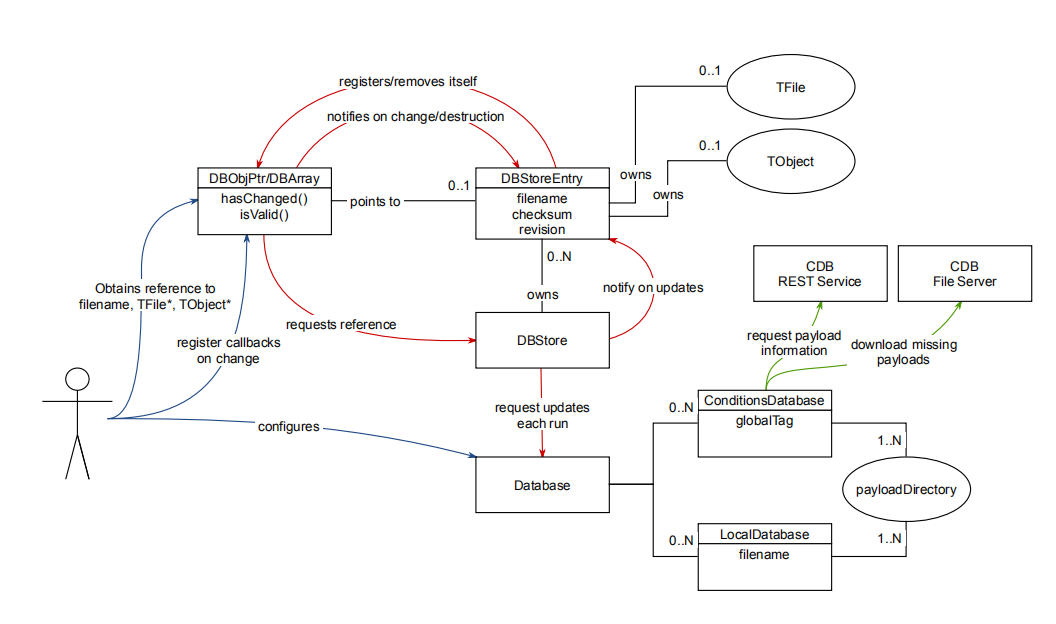
\includegraphics[height=9cm]{CDB}
\caption{ Relations of all entities in CDB\cite{BASF2}, showing the management logic from users' end to each CDB files and services. }
\label{fig:CDB}
\end{figure}
\end{comment}
 



\begin{comment}
The management of CBD with the extension of local database gives a good convenience for users to perform their own analysis and share the results with collaborators.
Users' access to conditions objects in the CDB is
provided by two interface classes, one for single objects
called ``DBObjPtr" and one for arrays of objects called
``DBArray". To facilitate easy creation of new conditions data – for example, during calibration – we provide two payload creation classes, ``DBImportObj" and ``DBImportArray". They
have an interface very similar to DBObjPtr and DBArray\cite{BASF2}.
\end{comment}

Users can create a GT, add objects of payloads to it and commit the GT to the configured database with a user-supplied IoV. This includes the support for run dependency as well. The capability to use a local file-based
database allows for easy preparation and validation of new payloads before they are uploaded to the CDB. Only the creator of the payload objects has the right to add, recall, replace and remove the GT from CDB, which guarantees the stability.

\begin{comment}
The scheme of this entities and how users interact with CDB object is demonstrated in Figure \ref{fig:CDB}. For example, user can perform their analysis and first locally generate weight files or calibration data based on different run conditions and reconstruction criteria, which are stated by their names of the IoVs. Once the results are good to share, they can create a GT in CDB of which they have the full ownership, add all database files into the GT and open it to Belle II collaboration. Anyone who would like to re-calibrate data or use their weight files for PID and so on, can simply use the built-in function ``basf2.useCentralDB()" in the BASF2 steering file to directly access the corresponding data. However, only the creator of the CDB objects has the right to add, recall, replace and remove the GT, which guarantees the stability of the CDB and responsibilities for each user.

\end{comment}

\begin{comment}
\subsection{Summary}
BASF2 has been developed for an emphasis on providing reliable and high quality performance for Belle II analysis. It satisfies the most of demanding requirements of data taking, simulation, reconstruction, and offline analysis. 
\end{comment}

\section{Belle II simulation}

This section briefly describes simulation (MC) used in the studies presented in this thesis. As this analysis is based on neutral $B$ meson, which is from the $\Upsilon$(4S) events, the  simulation is based on the electron -positron collisions at center-of-mass (CMS) energy $\sqrt{s} = 10.58 $ GeV.

In the previous section, it's shown that external packages and functionalities have been integrated with BASF2, including the core components of Belle II simulation in $B$ decay: \textit{evtgen} as event generator \cite{evtgen} and \textit{GEANT4} as the simulator of detectors \cite{agostinelli2003geant4}. For the simulation and the reconstruction used in this analysis, the latest release of BASF2 (release-05-01-01) was used. Based on the CDB management, BASF2 can utilize the same constants such as the magnetic field distribution for the consistence between simulation and reconstruction.

 All simulations start with at least one event generator that configures the physics processes. The \textit{evtgen} requires a decay file that describes the decay chain from a certain mother particle, branching fraction for all processes and decay-related information such as flavor mixing or $\it{CP}$ violation information. MC sample is centrally produced using Belle II grid computing service by DIRAC system and skimmed, of which the output is for physics analysis to create ROOT files. Each round of MC sample is packed and marked by their production index, such as \textit{MC13}, which is the latest MC sample with improvements in PID. In the following content of this thesis, all MC samples are produced in \textit{MC13} if not specifically stated. 
 
 For the analysis in this thesis, there are two MC samples included, where one is called \textit{signal MC} and the other is called \textit{generic MC}. \textit{Signal MC}, as its name suggests, is the MC sample that describes the whole decay chain of $B^0 \to K_S^0  K_S^0  K_S^0$. The mother particle of the decay chain is $\Upsilon$(4S), then it decays into a pair of $B^0-\bar{B}^0$ at branching fraction of 100\%, with the model \textit{EvtVSSMix}\cite{evtgen} describing the decay model. Then, one of the $B^0$ meson is set to decay into three $K_S^0$ based on phase-space model ($PHSP$) at 100\% branching fraction. The default configuration of evtgen can not handle multi-bodies charmless $B$ decay with TDCPV. A modified decay model profile is under-development and not fully validated yet. Thus, MC sample of $B^0 \to K_S^0  K_S^0  K_S^0$ yields zero $\it{CP}$ violation by default. As for the other $B$ meson, it decays into all possible final states that are described by the Belle II generic decay file. 
 
 As for \textit{generic MC}, all hadronic processes in a  $\sqrt{s} = 10.58 $ GeV collision are simulated. The total production cross section receives contributions from not only $\Upsilon$(4S) ($b$-flavor decay dominated), but also $u, d, s, c$. 
 Their relative branching fractions are taken from cross sections at  $\sqrt{s} = 10.58 $ GeV as shown in Table \ref{tab:generic_br}. \textit{Generic MC} sample contains 6 types of MC samples due to this production arrangement, where $\Upsilon$(4S) produces \textit{mixed} (neutral) and \textit{charged} $B$ meson pairs and the rest are other flavor mesons possibly with one extra photon emission named as $u\bar{u}(\gamma)$, $d\bar{d}(\gamma)$, $s\bar{s}(\gamma)$, and $c\bar{c}(\gamma)$, respectively. In this thesis, the latter 4 types of MC samples are combined and called $q\bar{q}$ for simplicity. In the mixed MC sample, the branching fraction of $B^0 \to K_S^0  K_S^0  K_S^0$ is set at $6 \times 10^{-6}$ and the branching fraction of $K_S^0 \to \pi^{+}\pi^{-}$ is set at 0.692. Both values are taken from Particle Data Group (PDG) \cite{pdg}. As the same as \textit{signal MC}, $\it{CP}$ violation is set to zero for signal events in \textit{generic MC} since they use the same model at generator level.
 
 \begin{table}
 	\caption{Production cross section for different hadronic flavors from collision at  $\sqrt{s} = 10.58 $ GeV used in Belle II \textit{generic MC} \cite{b2book}.}
 	\label{tab:generic_br}
 	\centering
 	\begin{tabular}{c|c|c|c|c|c}
 		\hline 
 	Processes & $\Upsilon$(4S) & $u\bar{u}(\gamma)$ & $d\bar{d}(\gamma)$ & $s\bar{s}(\gamma)$ & $c\bar{c}(\gamma)$ \\
 		\hline 
 	Cross section [nb] & $1.110\pm0.008$ & 1.61 & 0.40 & 0.38 & 1.30 \\
 	\hline
 	\end{tabular}
 \end{table}
 
In addition to the simulation of physics processes,  simulated data is produced with at least two beam background conditions, called \textit{BG0} without beam background and \textit{BG1} with one overlay of beam background. The components of them have been discussed briefly in section 2.7. The mixing of simulated beam background to simulated physics events is done by adding simulated hits on each sub-detector output. Possible pile-up of hits is therefore inherently included. The average number of background events of a given type to be added to a single simulated event is determined from the rate $R_{BG}$ of beam background sample and the time window $\Delta t$ in which the background is mixed shown in Equation \ref{bkgn}:

\begin{equation}\label{bkgn}
	\bar{N} = sR_{BG}\Delta t
\end{equation}
where $s$ is an optional scaling factor. The injected background events are based on a Poisson distribution with mean $\bar{N}$. Within the timing window, the background events are shifted randomly to simulate contributions from different bunches. To use real experiment background events (data-based beam background), the random triggered events are measured and added to
simulated $BG0$ MC sample for a more precised background configuration. This method can give a more realistic description of actual beam background but with a possibility to introduce bias due to the pile-up effect of multiple background events in a short timing window. In the early stage of the Belle II, the level of background is not high and the background pile-up effect is small.

In total, there are 2 million events generated in \textit{signal MC}. Half of the \textit{signal MC} (1 million) is produced without beam background for cross-checking the reconstruction performance. For \textit{generic MC}, 1 ab$^{-1}$ sample including mixed, charged and $q\bar{q}$ events are produced with beam background at  $\sqrt{s} = 10.58 $ GeV. The MC sample used in this analysis is summarized in Table \ref{tab:mc_all}

\begin{table}
	\large
	\caption{MC samples with and without beam background used in $B^0 \to K_S^0  K_S^0  K_S^0$ analysis.}
	\label{tab:mc_all}
	\centering
	\begin{tabular}{c|c|c}
		\hline 
		Events number & BG0 & BG1 \\
		\hline
		\textit{\textit{signal MC}} & $10^6$ & $10^6$ \\
		\hline
		\textit{\textit{generic MC}} & None & 1 ab$^{-1}$\\
		\hline
	\end{tabular}
\end{table}


\section{Belle II data taking}
The Belle II beam test operation started in 2016 which was focused on the commissioning and test of the SuperKEKB accelerator. Later in 2018, the commissioning of the Belle II detector was accomplished, with partial installation of PXD and full installation of SVD. From 2019 April, the physics run operation has officially started. The rest of the PXD is scheduled to be installed in 2023. By the end of 2020, Belle II has been operating for 4 total run seasons. The integrated luminosity collected during this period of time is about 84.73 fb$^{-1}$, shown in Figure \ref{fig:b2lumi}. The indices of physics runs are labeled which are experiment 7,8,10 for 2019 data taking and experiment 12 and 14 for 2020 data taking, as shown in Figure \ref{fig:b2lumi}. The data processing is regularly performed along with the data taking. For the analysis reported in this thesis, the experimental data collection from experiment 7, 8, 10 and 12 is used. Correspondingly, the integrated luminosity for offline reconstruction used in this thesis is about 62.8 fb$^{-1}$\cite{b2onlinelumi}. The experiment 14 is not used due to the unfinished processing of the latest experiment data. 

\begin{figure}
	\centering
	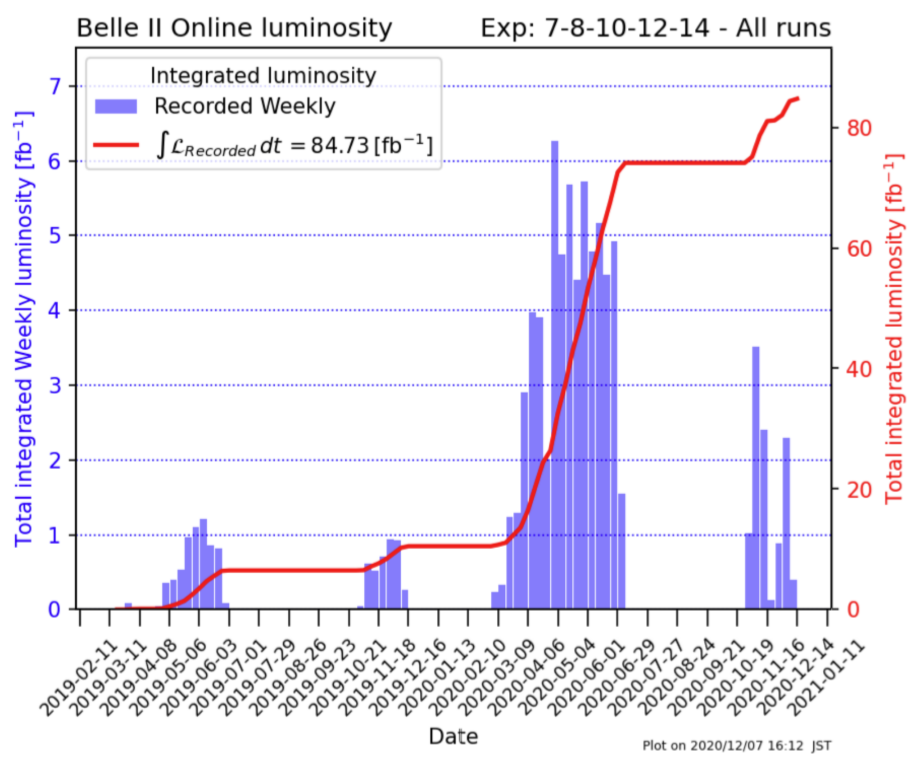
\includegraphics[width=0.6\linewidth]{b2lumi}
	\caption{Belle II online luminosity from 2019 April to the end of 2020. The experiment 7 and 8 were conducted during 2019 March to June. The experiment 10 was conducted during 2019 October to 2019 November. The experiment 12 was conducted during 2020 February to June. The experiment 14 was conducted during 2020 September to November.}
	\label{fig:b2lumi} 
\end{figure}
% 2021.02.01 ends
\chapter{$K_S^0$ reconstruction study}

The final states of $B^0 \to K_S^0  K_S^0  K_S^0 $ only depends on the decay of $K_S^0$. The main decay channels of $K_S^0$ is to either $\pi^+ \pi^-$ at branching fraction of about 0.692, or to $\pi^0 \pi^0$ at branching fraction of 0.307, referenced from PDG\cite{pdg}.
 The characteristics of these two decays are much different in terms of the response from the Belle II detector. The charged decay that yields  $\pi^+ \pi^-$ leaves two tracks originating from VXD or CDC volumes with opposite charges. On the other hand, the $\pi^0$ main decay channel is $\pi^0 \to \gamma \gamma$ which typically results in the photon clusters on the ECL. There are mainly two reasons for not selecting $\pi^0$ as final states.
 First, $\pi^0 \to \gamma \gamma$ can yield a large fraction of fake $K_S^0$. The reconstruction of two photons using ECL clusters provides no constrain on $K_S^0$ vertex so it's almost impossible to suppress the combinatorial background using vertexing quality in this case. The photons could be originating from many other resources, such as beam background and charged track radiation. Besides, the main viable selection is the mass of $K_S^0$ which is typically distributed around its nominal mass with a few hundred of keV. However, using the mass window of $K_S^0$ could not effectively reject the noticeable fraction of fake $K_S^0$, especially when using photons. Second, $B^0$ that decays to one or more $K_S^0$ reconstructed from neutral pions have poorly reconstructed vertices. Even with $B^0 \to K_S^0  K_S^0  K_S^0 $ which only uses $K_S^0$ from charged pions in the final states, there is no direct charged tracks from IP, which leads to the worse resolution of vertex position compared to the channel like a $B^0 \to J/\psi K_S^0$, which has two direct charged tracks of $e^+e^-$ or $\mu^+ \mu^-$ from $J/\psi$. If one (or more) of $K^0_S$ has the poor vertexing quality from its decay products, it can further reduce the precision of vertex positions of $B^0$, which eventually leads to a large uncertainties in defining the decay time of signal $B^0$ and the decay time difference as the key observables of TDCPV measurement. Therefore, only $K_S^0$ reconstructed using charged pions is considered to reconstructed $B^0$ in this analysis.
 
 \section{Cut-based $K_S^0$ Reconstruction}
 
 The $K_S^0$ has average life time at $(8.954 \pm 0.004) \times 10 ^{-11} \:\text{s}$ in PDG. Therefore, the flight length of $K_S^0$ is comparable with the scale of VXD size. In the Belle II energy scale, the flight length of $K_S^0$ is in a range from a few $\mu$m away from $B$ vertex to more than 13.5 cm that is further than the outmost layer of SVD ladders, see Figure \ref{fig:ks_flight}.

 % check this plot for how to normalize
 \begin{figure}[htpb]
 	\centering 
 	\begin{minipage}[t]{0.45\linewidth}
 	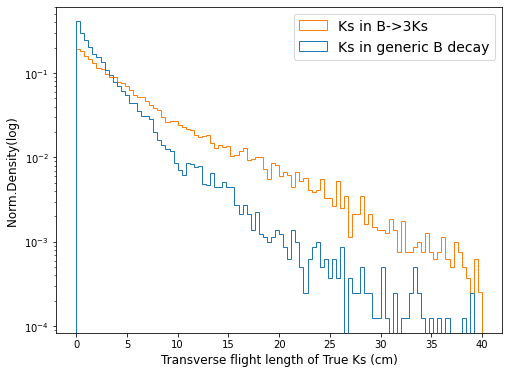
\includegraphics[width=0.9\linewidth]{ks_flight_XY}
 	\end{minipage}
	\begin{minipage}[t]{0.45\linewidth}
		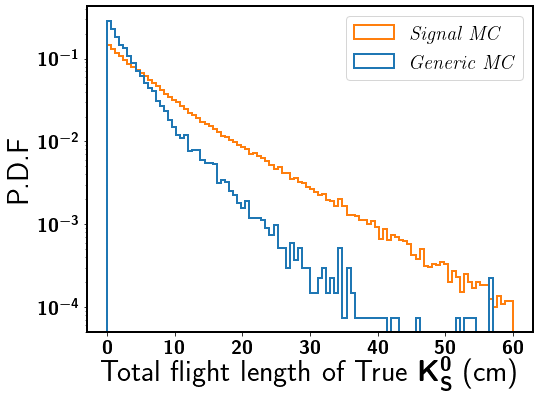
\includegraphics[width=0.9\linewidth]{ks_flight_All}
	\end{minipage}
 	\caption{The left is the transverse flight length distribution and the right is the total flight length distribution from true $K_S^0$.  The blue is from generic MC and  the orange is from signal MC. Both plots are normalized.}
 	\label{fig:ks_flight}
 \end{figure}
 
 Due to the different topology of $B^0$ decay, the average momentum of $K_S^0$ in generic MC is different from the ones from the signal MC. In general, the cut-based reconstruction for $K_S^0$ is first performed by the selection of invariant mass from its decay products. After the selection on invariant mass is applied, a vertex fit for each $K_S^0$ using two reconstructed charged pions is done without IP constraint. This reconstruction is mainly achieved by using standard BASF2 particle list, in which two $K_S^0$ collections are first reconstructed and then merged. We first take all the V0 objects from BASF2 which use 2 online reconstructed charged tracks with opposite charges and a converged fitted vertex. In this step, charged tracks with mass hypothesis of $\pi^{\pm}$ is used, which the tracks and PID of charged pions are pre-selected by the criteria in Table \ref{tab:kspipi_select}. The $K_S^0$ candidates with invariant mass $M$ between $0.45 < M < 0.55$ GeV are selected. In addition to these $K_S^0$ from V0 objects, another $K_S^0$ collection from offline reconstruction is also formed. The V0 based $K_S^0$ and offline reconstructed $K_S^0$ are merged and the vertex fit is performed using ``TreeFit"\cite{krohn2020global}. The duplication of $K_S^0$ between two $K_S^0$ collections are possible. Therefore, the objects' index of two charged pions' tracks in BASF2 are compared, from which the identical combinations are removed to avoid duplication. The $B^0$ reconstruction efficiency is highly sensitive to the efficiency of charged pions because the final state particles are three identical $K_S^0$ decaying to six charged pions. That's why a very loose selection on $\pi^{\pm}$ is applied. The selected $K_S^0$ collection using cut-based method contains many fake candidates from signal MC as shown in Figure \ref{fig:ksM_sigmc}.
\begin{table}[htbp]
	\centering
	\large
	\caption{Pre-selection criteria of $\pi^+ \pi^-$ for $K_S^0$ reconstruction.}
	\label{tab:kspipi_select}
	\begin{tabular}{c c c c }
		\toprule
		Selection & $\theta$ & CDC Hits Number & PID  \\
		\hline
		Criteria  & CDC acceptance &  $>20$ & pionID $> 0.1$\\
		\bottomrule
	\end{tabular}
\end{table}

% check y-axis and how many ks here.
\begin{figure}[ht]
	\centering 
	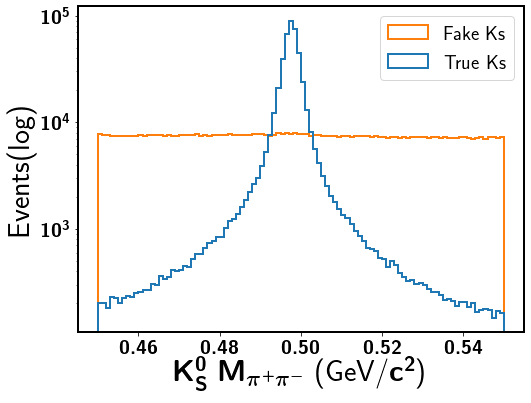
\includegraphics[width=0.6\linewidth]{Ks_M}
	\caption{``M" of $K_S^0$ from cut-based selection in signal MC. The blue line is the true $K_S^0$ and the orange is the fake $K_S^0$. 200000 candidates are used in total. }
	\label{fig:ksM_sigmc}
\end{figure}
\begin{comment}
The $K_S^0$ candidates from ``stdKshort:merged" is the default way to obtain $K_S^0$ in the current BASF2, 
however, the limitation of this cut-based $K_S^0$ reconstruction is the pollution from fake $K_S^0$. Using these $K_S^0$ candidates to reconstruct $B^0 \to K_S^0  K_S^0  K_S^0$, as long as one of three $K_S^0$ is fake, the reconstructed $B^0$ is fake, too. 
\end{comment}

 The reconstruction quality of $K_S^0$ also depends on the flight distance. $K_S^0$ that decay in the inner region of VXD yields more hits on the SVD layers from its charged daughters, which is critical in performing a proper tracking. Belle II tracking efficiency gets poor due to higher beam background when performing track finding for tracks without inner detector hits such as SVD. For certain fraction of $K_S^0$ decaying outside of layer 5 of SVD, it's much likely that there is no SVD hits assigned to their daughters' tracks. This is due to the feature of SVD track finding, where a track candidate needs either at least 3 SVD hits to form a good SVD track, or 2 hits to form a hit double-lets to be used as a complete track. Single hit on layer 5 or layer 6 is filtered out to suppress the large fraction of beam background induced by random single hits. This effect is shown in Figure \ref{fig:ks-r-svdxx}. $K_S^0$ are categorized based on how many SVD hits their daughters have, in which \textit{SVD10} and \textit{SVD01} stands for $K_S^0$ that only $\pi^+$ and $\pi^-$ has non-zero SVD hits number, \textit{SVD11} and \textit{SVD00} stands for $K_S^0$ that both or neither charged pions have SVD hit non-zero SVD hits number. This is related to the track quality of $K_S^0$ where \textit{SVD11} $K_S^0$ has the best quality and \textit{SVD00} has the worst. Thus, the efficiency and purity of $K_S^0$ with long flight length is reduced. It's clear that \textit{SVD00} $K_S^0$ show up at about 11 cm where SVD layer 5 is placed. Most of \textit{SVD10}(\textit{SVD01}) $K_S^0$ start to show up at the similar range. The geometric structure of PXD and SVD is shown in Figure \ref{fig:svdgeo} and the fraction for each types of $K_S^0$ in $B^0 \to K_S^0  K_S^0  K_S^0$ is listed in Table \ref{tab:svdxx}.
\begin{figure}[htpb]
	\centering
	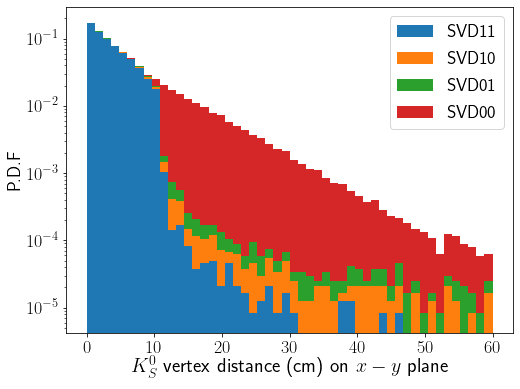
\includegraphics[width=0.7\linewidth]{ks-r-svdxx}
	\caption{$K_S^0$ transverse flight length based on SVD hits of pions. \textit{SVD11}: both pions have SVD hits, \textit{SVD10}(\textit{SVD01}), positive(negative) pions have SVD hits, and \textit{SVD00}: no SVD hits from pions. The result is from signal MC of $B^0 \to K_S^0  K_S^0  K_S^0$.}
	\label{fig:ks-r-svdxx}
\end{figure}

\begin{table}[H]
	\centering
	\begin{tabular}{|c|c|c|c|c|}
		\hline
		$K_S^0$ type & SVD11 & SVD00 & SVD10 & SVD01\\
		\hline
		\% in Belle II & 52\% & 39\% & 5\% & 5\%\\
		\hline
	\end{tabular}
	\caption{The fraction of each category of $K_S^0$ based on pions SVD hits in $B^0 \to K_S^0  K_S^0  K_S^0$ signal MC.}
	\label{tab:svdxx}
\end{table}
\begin{comment}
\begin{figure}[htpb]
\centering
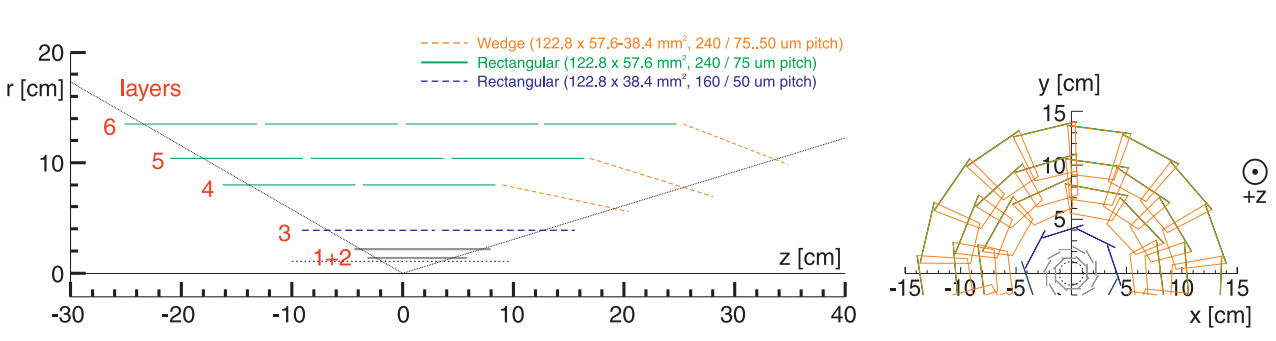
\includegraphics[height=4cm]{VXDGEO.png}
\caption{Geometric structure of PXD and SVD in Belle II\cite{Abe:2010gxa}. SVD Layer 5 is at $r = 11$ cm and $K_S^0$ that decay outside are very likely to lose SVD hits information.}
\label{fig:vxdgeo}
\end{figure}
\end{comment}


Fake $K_S^0$ candidates costs a large extra processing time and the number of combinatorial backgrounds in $B^0 \to K_S^0  K_S^0  K_S^0$ becomes high, which largely reduces the signal significance and introduce bias to the $\it{CP}$ parameters measurement. Thus, a multi-variate analysis (MVA) based $K_S^0$ classification package, \textit{KsFinder}, is developed to further reject the fake $K_S^0$ from cut-based selected candidates.


% 2021.02.03 ends
\section{MVA-based $K_S^0$ selection}

\subsection{Belle II $K_S^0$ classification}
As mentioned in the last section, in order to improve the reconstruction performance of $K_S^0$ from cut-based selection, a MVA-based package called ``KsFinder" has been developed. The reconstruction of $K_S^0$ can be treated as a typical classification problem. The input is a set of variables that describes the characteristics of $K_S^0 \to \pi^+ \pi^-$ decay. The training  target is the true or fake flag from the MC truth-matching variable called ``isSignal" where isSignal = 1 (0) stands for being a true (fake) $K_S^0$. It aims to improve the limitations in the Belle $K_S^0$ MVA classification tool. 
 
 In Belle, the $K_S^0$ reconstruction was first done by using cut-based method to select primary candidates, then a MVA-based classifier was implemented by assigning two likelihood indicators to each $K_S^0$ candidates. The package used by Belle is called \textit{nisKsFinder}\cite{b2book} which outputs the two likelihood variables based on NeuroBayes algorithm\cite{feindt2006neurobayes}. The Belle tool defines the goodness of $K_S^0$, called \textit{nb\_nolam} and \textit{nb\_vlike}, respectively. As their names suggest, \textit{nb\_nolam} is the likelihood of not being a $\Lambda$ particle and \textit{nb\_vlike} is the likelihood of being a V0-like particle. A good $K_S^0$ candidate from \textit{nisKsFinder} is the one with a low likelihood of being $\Lambda$ particle and a high likelihood of being a V0-like particle, assuming the major backgrounds for $K_S^0$ is the mis-identified $\Lambda$ among V0-like particles. By putting cuts on these two variables, a purification of $K_S^0$ can be made, see Figure \ref{b1niskf}. It can effectively reduce fake $K_S^0$ from cut-based selected candidates, however, there are a few disadvantages about this method. First, NeuroBayes is a commercial product that was developed over 10 years ago. The official support and update is stopped nowadays, so it's not an ideal method for an experiment like Belle II that has a quite long prospective in operation. Second, the classification is based on a joint cut on two variables, which might make the cut values hard to choose, for example, two different cuts might have very close purity. Last but not least, the classification of $K_S^0$ is not the directly targeted output of the neuro-network. Instead, it classifies the V0-like particle and ``$\Lambda$". Besides, the computation speed of NeuroBayes is not optimized.

\begin{figure}[htpb]
	\centering 
	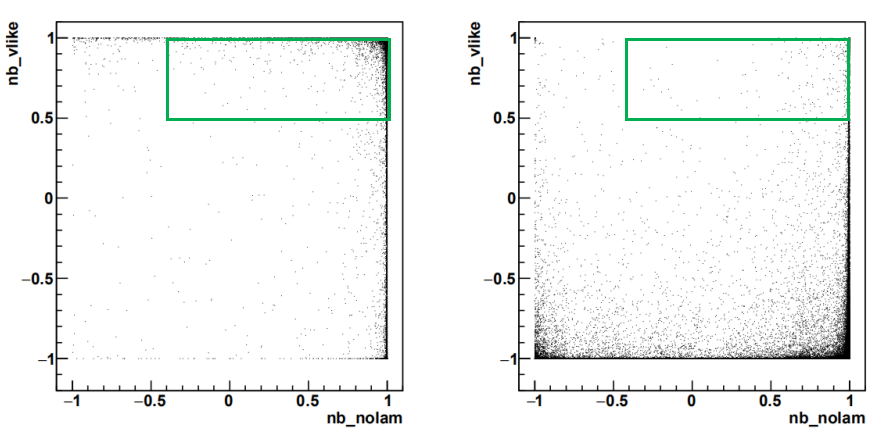
\includegraphics[width=0.7\linewidth]{nisksfinder}
	\caption{The distribution of two variables outputs: \textit{nb\_nolam} and \textit{nb\_vlike} for $K_S^0$ candidates from Belle signal MC. The left is from true $K_S^0$ and the right is from the fake $K_S^0$. In Belle, the standard cuts for $K_S^0$ is \textit{nb\_vlike} $> 0.5$ and \textit{nb\_nolam} $> -0.4$\cite{kang2020measurement}.}
	\label{b1niskf}
\end{figure}


Such a dedicated $K_S^0$ classification tool is not implemented yet in BASF2 framework until 2019. Considered the limitation of NeuroBayes, the development of $K_S^0$ classifier demands another algorithm and structure. The \textit{Boosted Decision Trees} (BDT) is widely employed for multivariate classification and regression tasks in high energy physics field. Particularly, a speed-optimized and cache-friendly
implementation of such a method called FastBDT (FBDT) is popularly used\cite{keck2016fastbdt}. Compared to other popular classification algorithms such as TMVA\cite{therhaag2012tmva}, scikit-learn\cite{pedregosa2011scikit} and XGBoost\cite{chen2016xgboost}, FastBDT method is proven to be one order of magnitude faster during the training and applying phases\cite{keck2016fastbdt}. 
By using FastBDT algorithm, KsFinder in Belle II is expected to give a single output which directly presents the goodness of a candidate of being a true $K_S^0$. Since the FastBDT algorithm depends on the variables that are different in signal and backgrounds, a set of training variables are selected based on $K_S^0$ decay topology.  The $K_S^0$ variables used in the training of KsFinder might be differently distributed in different decay channels, therefore a KsFinder trained using MC sample from one channel may not be able to perform a good classification on the other. Thus, KsFinder is designed as a general package that provides a mode-dependent $K_S^0$ classification which mainly consists of four components: \textit{KsFinderSampler}, \textit{KsFinderTeacher}, \textit{KsFinderApplier} and \textit{KsFinderTest}. KsFinderSampler is a function that automatically generates training and/or testing sample from mDST files where the cut-based reconstruction is used as section 3.1. KsFinderTeacher is responsible for extracting variables to perform training of the FastBDT model and generate a weight file containing all the nodes information in ROOT format, which also provides a function to communicate with BASF2 CDB so that users can share or download others' weight file in their own analysis. KsFinderApplier can apply the weight file generated by KsFinderTeacher (or downloaded from BASF2 CDB) to the independent data sample and assign each $K_S^0$ candidate a goodness index used as a single cut value in the further analysis. KsFinderTest is the evaluation function that can use a test sample to check for over-training, efficiency, purity.  By providing MC sample(s) from a certain decay mode(s), users can easily generate their own weight file(s) of $K_S^0$ classification that suits different decay modes despite $K_S^0$ variables distribution may be varied. Such a design largely improves the flexibility of KsFinder compared to Belle MVA tool which indirectly classify $K_S^0$ with two outputs. 

\begin{comment}
\subsection{FastBDT algorithm}
As the basic component of BDT, a general DT (decision tree) performs classification using a number of consecutive cuts at each tree nodes, where tree nodes are distributed on the layers of a tree. The maximum number of the layers is called ``depth of tree" and it's a hyper-parameter of a DT. Each data point contains labels (variables) called ``features" in DT. There are generally two phases in using DT for classification. One is ``training" (or ``fitting") phase that determines the best cut at each nodes. The other is called ``applying" phase that uses a trained DT to classifier a new data set. In training phase, training data points are fed to a DT and separated based on their features. At each node with a cut value, a cumulative probability histogram (CPH) can be defined by counting the signal and background data points. The histograms are used to determine the separation gain for a cut value at each position in these histograms. The feature and cut value (or
equivalently bin) with the highest separation power are used as the cut for the node. Hence, each cut value locally maximizes the separation gain between signal and background on the given
training sample. Eventually, on the last layer (called terminal layer), the signal fraction of all training data points in the same terminal node is used for the signal probability for a testing data point which ends up in the same terminal nodes, shown as Figure \ref{fig:DT}. In applying phase, a new data set, such as a test sample, is fed to the trained DT with fixed cut values at each nodes, to evaluate the performance of a DT or use it to separate the signal and background.

\begin{figure}[htpb]
\centering 
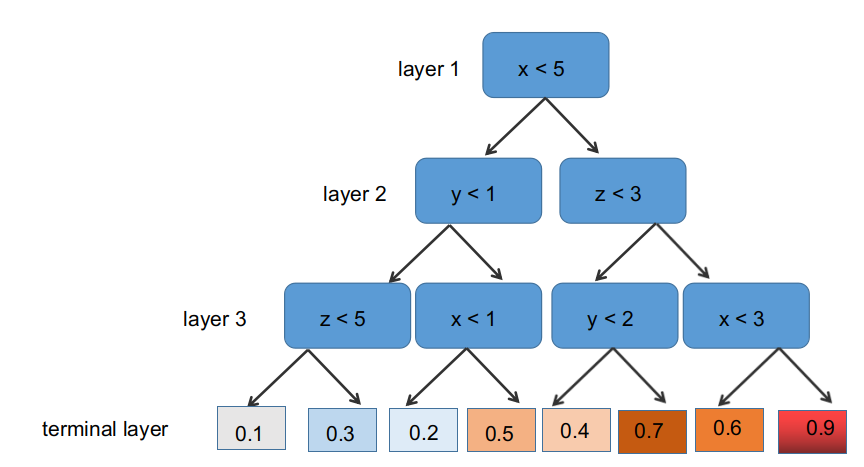
\includegraphics[width=0.7\linewidth]{DT}
\caption{Basic structure of a DT with depth = 3 and labels (features) of x,y,z. The terminal layer contains training data points and are separated by cuts on layer 1 to 3. The number (color demonstrated) is the signal fraction of training data points in each terminal node, which is used for testing data points signal probability.}
\label{fig:DT}
\end{figure}

The mathematical idea behind this method is to treat the data points as a data set defined on a multi-dimension hyper-space. As long as the signal/background data points show certain concentration in a sub-region of the hyper-space, it's possible to locally increase the signal fraction by consecutively cutting on the edge where signal and background are separated. The cut on labels at each node is the edge of the sub-region. A very deep DT (too many layers) means the edges of the sub-region of the hyper-space is cut too finely so that even small statistical fluctuation could be separated. Therefore, training data points in the sub-region can give a over-trained signal fraction that is unrealistically high. As a result, the classifier performs poorly on new data points since the fluctuation is randomly occurred in new data set. There are pruning algorithms which automatically remove cuts prone to over-training
from a DT, details can be found here \cite{olshen1984classification}.

Avoiding the over-training of a DT limits the depth of a tree strongly. For a problem of $K_S^0$ classification, the number of observables (features) is much more than the usual tree depth (a few layers). A single DT can only roughly separate the signal and background and thus, it's called a weak-learner. To improve the separation power, a sequence of many shallow DTs is formed during the training phase. For all the DTs, a negative binomial log-likelihood loss-function is minimized in the training phase. By using the results from many DTs (many weak learners), a well-regularized classifier with large separation power is constructed. The number of trees $N$ is called ``boosting steps", which is also the hyper-parameters for the training model. Such improved model is called ``Boosted Decision Trees" (BDT). There are a few different strategies to further optimize the performance of BDT such as ``Gradient Boost Decision Trees" (GBDT) and ``Stochastic Gradient Boost Decision Trees" (SGBDT) which use different methods to define the model output or increase the training speed, details are discussed here\cite{friedman2002stochastic}.


The FastBDT (FBDT) implements a optimized algorithm from a derived SGBDT method \cite{friedman2001greedy} and gain an order of magnitude faster execution time. FBDT reduces CPU time on CPH for tree nodes by using binned values for comparison to avoid  floating-point data calculation. It uses ``struct of arrays" that leads to a faster pre-cached CPU memory access pattern. The comprehensive comparison in terms of speed in fitting and applying phases between FastBDT and other popular methods such as XGBT, TMVA and scikit-learn is described in here\cite{keck2016fastbdt}. 

\begin{comment}
\begin{figure}[htpb]
\centering
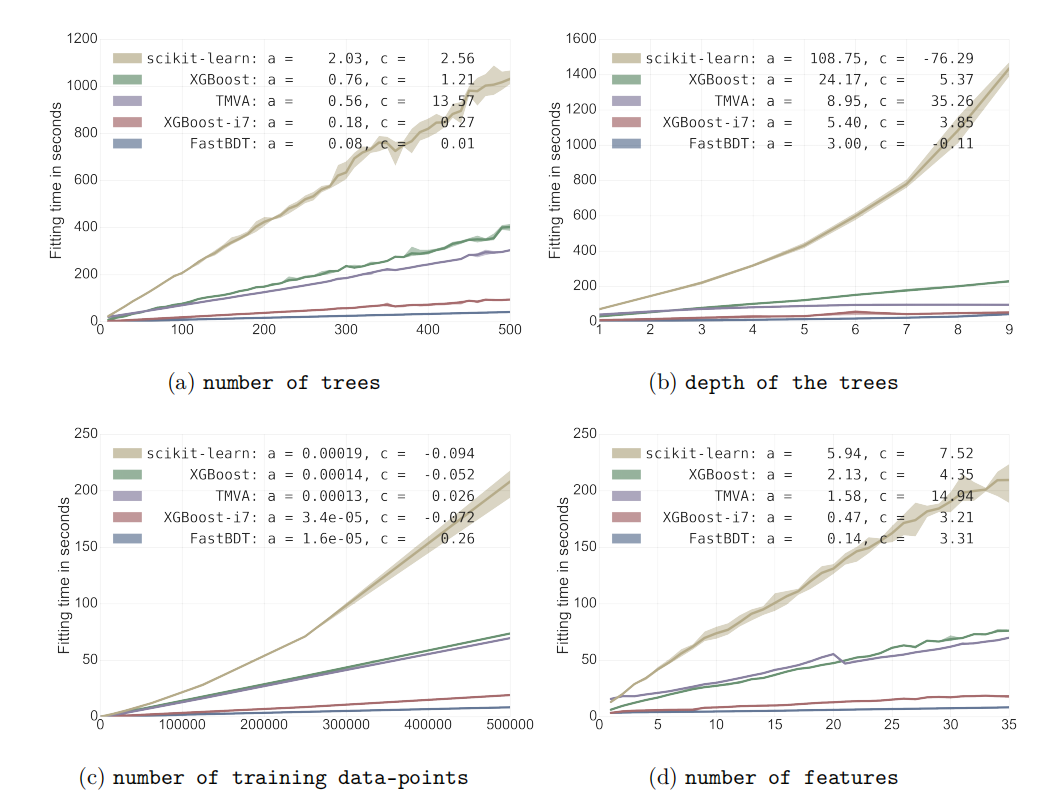
\includegraphics[height=12cm]{speedFBDT}
\caption{Runtime in fitting phase with different hyper-parameters comparison among FastBDT and XGBT,TMVA,scikit-learn.\cite{keck2016fastbdt}}
\end{figure}
\end{comment}

% 2021.02.04 ends


\subsection{Decay Topology of $K_S^0 \to \pi^+ \pi^-$}
As introduced in section 3.2.1, the first step for developing $K_S^0$ MVA classification is to determine the input variables for FastBDT algorithm that can represent the decay features of $K_S^0$ against possible backgrounds.
The remaining background of  $K_S^0 \to \pi^+ \pi^-$ after the cut-based reconstruction comes from different sources, mainly including the false combination of tracks (including $\pi^{\pm}$ misidentification), V0-like particle misidentification and self-looped tracks.
For instance, a $D^0/D^*$ from a $B$ decaying to $K\pi$ with $K$ misidentified as $\pi$, could give a false combination of tracks. On the other hand, it's also possible that both of two tracks are correctly identified as $\pi^{\pm}$ but they are not from the same mother particle, or the mother is not a $K_S^0$ particle due to the missing of other daughters, such as $D^+ \to K_S^0 (  \to \pi^+ \pi^-) \pi^+$. The decay shape resembled the above cases are illustrated in Figure \ref{fig:fakeks1}. 


\begin{figure}[htpb]
	\begin{minipage}[t]{0.5\linewidth} % 如果一行放2个图,用0.5,如果3个图,用0.33
		\centering 
		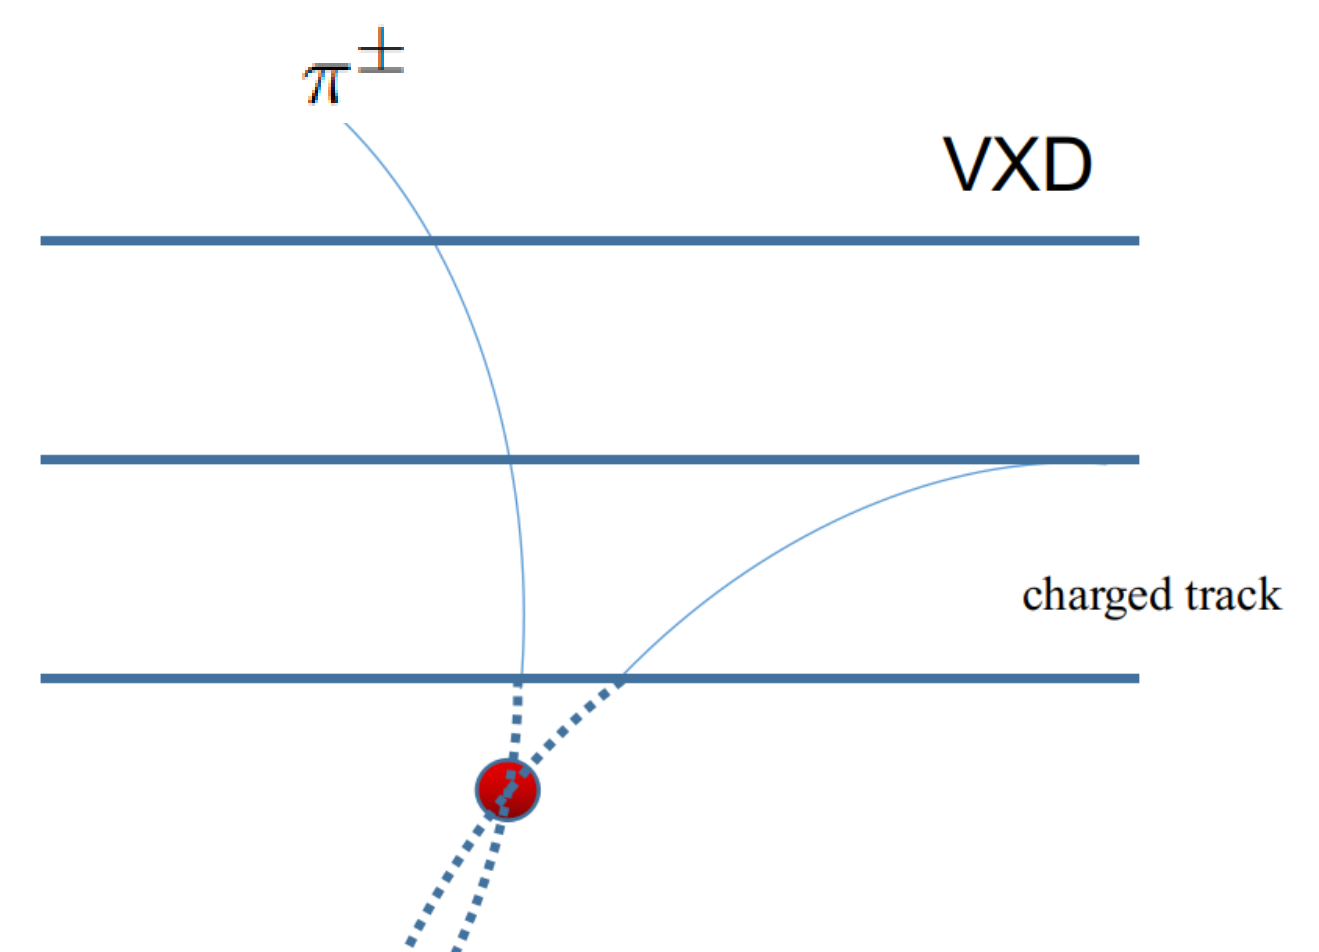
\includegraphics[width=7cm]{fakeks1_1} 
		%\label{fig:side:a} 
	\end{minipage}%
	\begin{minipage}[t]{0.5\linewidth} 
		\centering 
		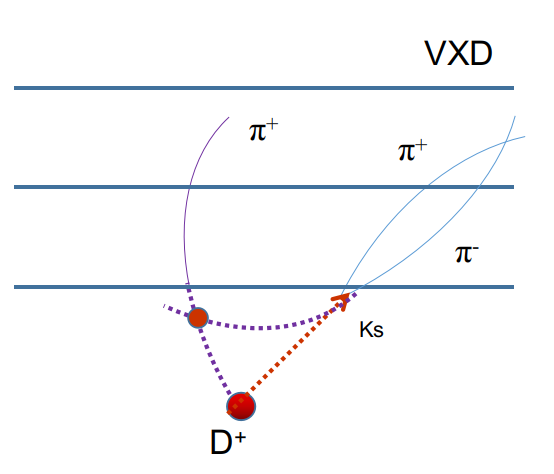
\includegraphics[width=7cm]{fakeks2} 
		%\caption{ } 
		%\label{} 
	\end{minipage}% 
	
	\caption{The left shows the case when a charged track (not $\pi^{\pm}$) combined with a charged pion to form a fake $K_S^0$, the right shows the case when two daughters are correctly reconstructed as pions but not from the correct mother particle, which is falsely taken as a $K_S^0$.}
	\label{fig:fakeks1}
\end{figure}

The V0-like particles mainly refer to $K_S^0$, $\Lambda$ and $\gamma$. $\gamma \to e^+ e^-$ yield is significantly lower than the other two types and the mass different between pion and electron is very large, so the PID values can be used to well-distinguish them. As for the contribution of $\Lambda \to p^+ \pi^-$, it happens when the positive charged tracks (proton track) is wrongly identified as $\pi^+$, see Figure \ref{fig:fakeks2} left. The key observable to distinguish this background is the invariant mass of mother particle, which is 1.115 $\Lambda$ GeV, much larger than the $K_S^0$. The number of left-over $\Lambda$ after the cut-based reconstruction in section 3.1 is small, and can be further reduced by rejecting the candidates whose positive charged daughter has PID($\pi^{\pm}$) smaller than PID($p$).

When a charged pion only carries a minimal of its mother's transverse momentum $p_T$, the curvature of its track may form a self-loop of which radius is comparable with the size of Belle II detector (mainly VXD and CDC). In this case, one charge pion could leave two charged tracks candidates with the opposite charge and similar $p_T$, with a possibility to form a converged vertex to form a fake $K_S^0$, see Figure \ref{fig:fakeks2} right.

\begin{figure}[htbp]
	\begin{minipage}[t]{0.5\linewidth} % 如果一行放2个图,用0.5,如果3个图,用0.33
		\centering 
		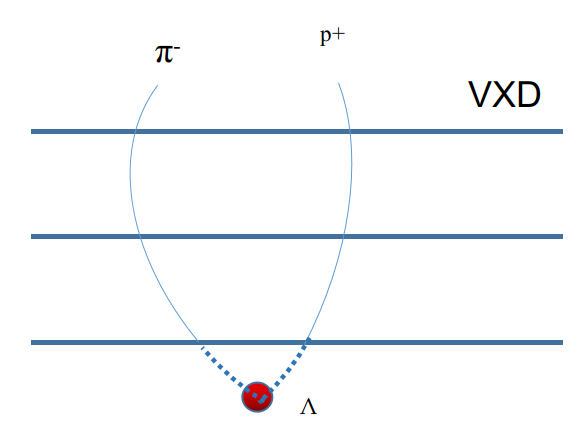
\includegraphics[width=7cm]{fakeks3} 
		\label{fig:side:a} 
	\end{minipage}%
	\begin{minipage}[t]{0.5\linewidth} 
		\centering 
		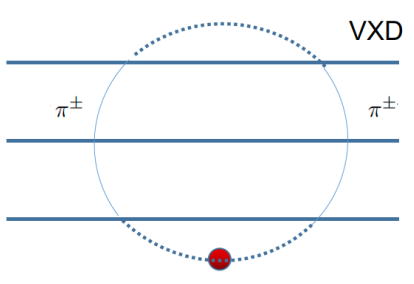
\includegraphics[width=7cm]{fakeks4_4} 
		%\caption{ } 
		\label{fig:side:b} 
	\end{minipage}% 
	
	\caption{The left shows the $\Lambda \to p^+ \pi^-$ decay shape that can be treated as $K_S^0$, the right shows a self-loop formed by a low $p_T$ charged pion reconstructed as two separated tracks with a vertex.}
	\label{fig:fakeks2}
\end{figure}

\subsection{Determination of training observables from $K_S^0$ decay }
Given the characteristics of  $K_S^0 \to \pi^+ \pi^-$ discussed in the previous section, a set of variables as training features of KsFinder can be selected. The set includes variables related to $K_S^0$ kinematics, decay shape parameters, particle identifications and detector hits information. The summarized information of training variables is listed in Table \ref{tab:ks_vars}.

\begin{table}[htbp]
	\centering 
	\small
	\begin{tabular}{|c|c|} 
		\hline
		$K_S^0$ variables &  Meaning \\
		\hline
		{cosVertexMomentum} & cosine between $K_S^0$ vertex and momentum direction (lab)\\
		flight distance & $K_S^0$ flight distance projected on its momentum direction\\
		significanceOfDistance & relative error of flight length from IP\\
		cosHelicityAngleMomentum & cosine between $\pi^{\pm}$ and $K_S^0$ (lab)\\
		ImpactXY & Impact parameters in transverse plane for $K_S^0$\\
		x, y, z, px, py, pz & $K_S^0$ vertex position and momentum\\
		p\_D1(D2) & momentum magnitude for $\pi^+$($\pi^-$)\\
		pionID, muonID & PID values of $\pi^+$\\
		decayAngle\_D1(D2) & angle between $\pi^+$($\pi^-$) and $K_S^0$ ($K_S^0$ CMS)\\
		daughterAngle2body & angle between $\pi^{\pm}$ (lab)\\
		daughtersDeltaZ & Z-direction distance of two tracks helix\\
		nSVDHits\_D1(D2)& SVD detector hits of  $\pi^+$($\pi^-$) \\
		nPXDHits\_D1(D2)& PXD detector hits of  $\pi^+$($\pi^-$) \\
		M, InvM & $K_S^0$ invariant mass before(after) vertex fit\\
		\hline
	\end{tabular}
	\caption{\small Summary of KsFinder input variables, where ``lab" means angles in lab frame and  ``$K_S^0$ CMS" means in $K_S^0$ rest frame. Other variables are calculated in lab frame by default. }
	\label{tab:ks_vars}
\end{table}

\begin{comment}
\begin{itemize}
\item Kinematics
\begin{itemize}
\item invariant mass of $K_S^0$ before and after fitting vertex
\item momentum of $K_S^0$ and $\pi^{\pm}$, vectors and magnitudes. 
\end{itemize}

\item Decay shape parameters
\begin{itemize}
\item cosine angle between $K_S^0$ vertex and momentum in lab frame.
\item helicity angle of two daughters in reference of $K_S^0$ momentum in lab frame.
\item decay angle of two daughters ($\pi^{\pm}$) in the mother's ($K_S^0$) frame. 
\item flight distance projection on $K_S^0$ momentum direction.
\item significance of flight distance, defined by ratio of flight length and its uncertainties.
\item distance of two daughters helix along the Z direction (parallel to beamline).
\item impact parameters on $K_S^0$ vertex
\end{itemize}

\item Particle identifications
\begin{itemize}
\item pion-ID for $K_S^0$ daughters.
\item muon-ID for $K_S^0$ daughters.
\item proton-ID for $K_S^0$ positive charged daughter. 
\end{itemize}

\item Hits information
\begin{itemize}
\item the number of PXD hits for each $K_S^0$ daughter.
\item the number of SVD hits for each $K_S^0$ daughter.
%\item the number of CDC hits for each $K_S^0$ daughter. 
\end{itemize}

\end{itemize}
\end{comment}

The cosine between $K_S^0$ vertex and momentum direction (named ``cosVertexMomentum") is of the most importance because it demonstrates the best separation between a true and a fake $K_S^0$. For instance, if a falsely reconstructed $K_S^0$ is made of two tracks, it's likely that the momentum direction of the fake $K_S^0$ is not aligned with the its vertex direction from IP. So the projection of vertex position of $K_S^0$ on the reconstructed momentum direction could be negative value for fake $K_S^0$. While in case of a true $K_S^0$, such projection is almost always a positive value, shown in Figure \ref{fig:ks_cosvex}. This often happens when the two tracks taken as $\pi^{\pm}$ are accidentally crossed, or due to the misidentified track(s). The abbreviations and importance rank of input variables from KsFinderTest function is shown in Table 
\ref{tab:ks_import}.

\begin{figure}[htbp]
	\centering
	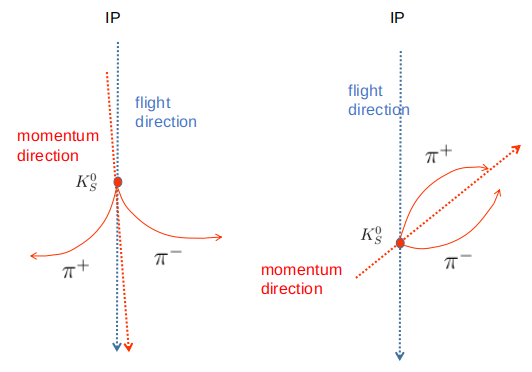
\includegraphics[height=7cm]{ks_cosvex}
	\caption{The left shows a true $K_S^0$ decay shape where the cosine angle of $K_S^0$ vertex position (blue dashed arrow) against reconstructed momentum direction (red dashed arrow) is positive. While the right shows a fake $K_S^0$ decay shape where cosine angle of $K_S^0$ vertex position against reconstructed momentum direction can be negative. }
	\label{fig:ks_cosvex}
\end{figure}
 
As a FastBDT method relies on the distribution of variables to calculate signal and background separation, there are a few points to be checked before feeding the training data to the algorithm or applying the classification. First, the distribution of the observables should be different in true $K_S^0$ and the fake ones, so the FastBDT classifier can effectively separate the true and the fake $K_S^0$ at each node to maximize the separation gain. Second, there will a correlation among the training observables and they should also be different in signal and background. The boosting step will create a sequence of shallow DTs whose structures are not same. Different correlations helps improve the performance of DTs in tuning of structure. For instance, a true $K_S^0$ flights longer due to larger momentum in general, so its daughters' detector hits number becomes fewer. Then these two observables have negative correlations in true $K_S^0$. In case a fake $K_S^0$, the flight length could be a deep outside of VXD  but daughters may have full hits on SVD, without strong correlation, see Figure  \ref{fig:ks_cov} . At last, one should also avoid using many observables with too strong correlations, since in this case, many DTs might have a potentially equivalent structure in the boosting step. Therefore, the separation power of many DTs doesn't gain any improvement and the collection of observables might be redundant. The correlation between variables are shown in Figure \ref{fig:ks_cov}.

\begin{figure}[ht]
\centering
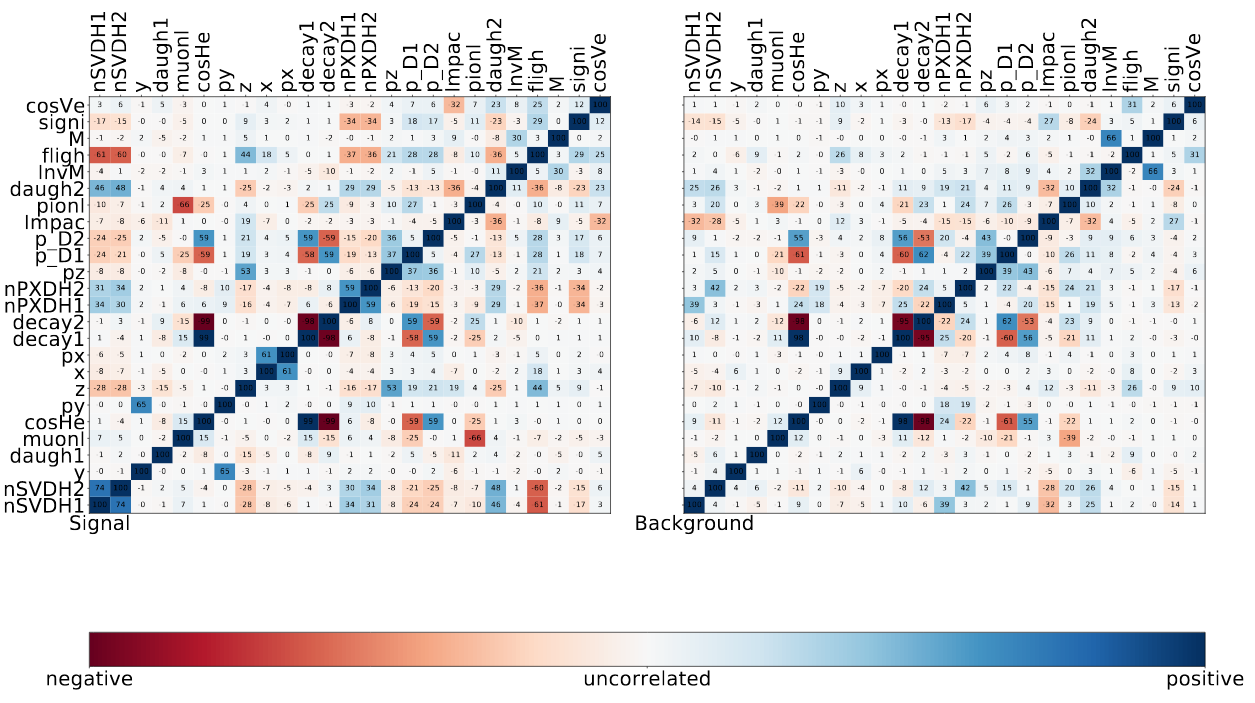
\includegraphics[width=0.8\linewidth]{ks_cov}
\caption{The correlation between input variables for KsFinder. As the given example, flight length has negative correlation with SVD hits in signal while un-correlated in background.}
\label{fig:ks_cov}
\end{figure}

 \begin{table}[htpb]
 	\begin{minipage}[ht]{0.5\linewidth}
 		\centering
 		%\caption{The Abbreviations.}
 		\begin{tabular}{c|c}
 			\hline
 			Observables &  Abbreviations\\
 			\hline
 			nPXDHits\_D1 &  nPXDH1 \\
 			decayAngle\_D1 & decay1 \\
 			nPXDHits\_D2 & nPXDH2\\
 			y & y \\
 			decayAngle\_D2 & decay2\\
 			px & px\\
 			z & z \\
 			cosHelicityAngleMomentum & cosHe\\
 			x & x \\
 			daughtersDeltaZ & daugh1\\
 			nSVDHits\_D1 & nSVDH1\\
 			py & py\\
 			muonID\_pi & muonI\\
 			nSVDHits\_D2 & nSVDH2\\
 			p\_D1 & p\_D1\\
 			p\_D2 & p\_D2\\
 			pz & pz \\
 			flightDistance & fligh\\
 			pionID\_pi & pionI\\
 			InvM & InvM \\
 			daughterAngle2body & daugh2\\
 			ImpactXY & Impac \\
 			significanceOfDistance & signi \\
 			M & M \\
 			cosVertexMomentum & cosVe \\
 			\hline
 		\end{tabular}
 		%\label{fig:side:a} 
 	\end{minipage}
 	\begin{minipage}[ht]{0.5\linewidth}
 		\centering 
 		%\caption{Importance rank }
 		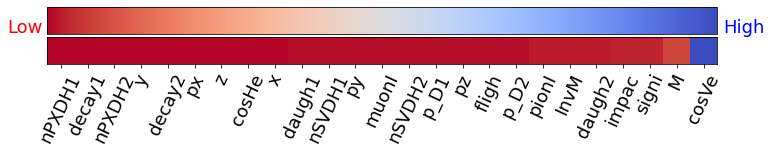
\includegraphics[width=4cm]{rank1}
 		%\label{fig:side:b} 
 	\end{minipage}
 \caption{The abbreviations (left) and importance rank (right) of input variables from KsFinderTest, where the most important variable is ``cosVertexMomentum".}
 \label{tab:ks_import}
 \end{table}




 % 2021.02.05 mid
\subsection{Training, Applying and Testing of KsFinder}
The variables are internally registered inside the KsFinder so it can automatically retrieve their values from a mDST file in BASF2. The first step of using KsFinder is to call KsFinderSampler on a MC sample to generate training and testing data sample. To show the flexibility and stability of KsFinder on different modes, KsFinderSampler extracts MC data points from both signal MC and generic MC (see MC definition in section 2.9), respectively.  KsFinder configures that the depth of each DT is 3 and boosting steps is 200. In both MC samples, the ratio of true and fake $K_S^0$ is set to 1:1 and each component contains 200000 data points. The distribution of input variables in signal MC is shown in Appendix A. 

To train the KsFinder, KsFinderTeacher function is called for the training samples from signal/generic MC and weight files are saved. To apply the classification of $K_S^0$, KsFinderApplier reads in the testing samples of signal/generic MC and calculate output using saved weight files, so that each $K_S^0$ candidate is assigned with a goodness index named \textit{FBDT\_Ks}. It ranges from 0 to 1 where 1 stands for the best goodness. After the applying of KsFinder on the testing samples, KsFinderTest is called to check the performance and over-training of KsFinder on the testing samples, which will be discussed in the next section. 

\subsection{The Performance and Over-fitting check}
To evaluate the performance of KsFinder on both signal and generic MC samples, signal efficiency and background rejection are calculated by cutting on the different values on \textit{FBDT\_Ks}, as defined in Equation \ref{eq:ks_eff} and \ref{eq:ks_rej}.

\begin{eqnarray}
	\text{signal efficency} = \frac{\text{Number of true $K_S^0$ with FBDT\_Ks $>$ cut value}}{\text{Number of all true $K_S^0$ }} \label{eq:ks_eff}\\
	\text{background rejection} = \frac{\text{Number of fake $K_S^0$ with FBDT\_Ks $<$ cut value}}{\text{Number of fake true $K_S^0$ }} \label{eq:ks_rej}
\end{eqnarray}

The ROC (receiver operating characteristics) curve is usually taken as an indicator of the performance where the curve shows the dependence of rejection power with respect to the signal purity. The larger area under a ROC curve means that the better performance is achieved since background rejection drops slower when increasing the cut. The ROC curves and efficiency/background rejections are shown in Figure \ref{fig:3Ks_performance} and \ref{fig:gen_performance}, where the former is for signal MC and the latter is for generic MC.

\begin{figure}[H]
	\begin{minipage}[b]{0.5\linewidth}
		\centering 
		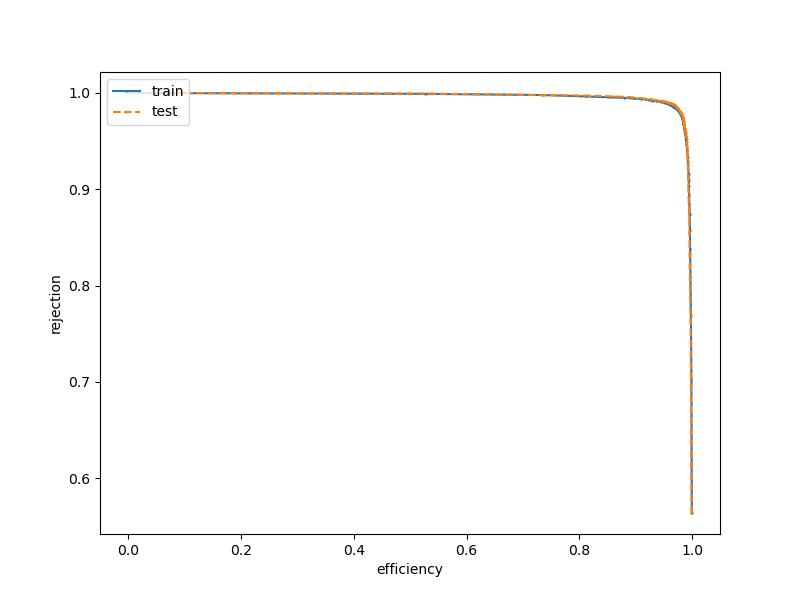
\includegraphics[height=6cm]{ROC_3Ks}
		\label{fig:ROC_3Ks}
	\end{minipage}
	\begin{minipage}[b]{0.5\linewidth}
		\centering 
		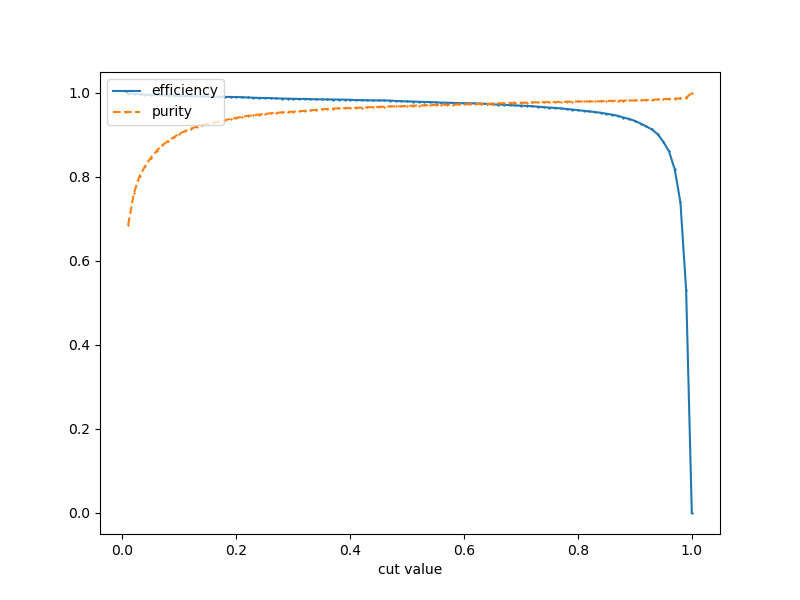
\includegraphics[height=6cm]{eff_3Ks}
		\label{fig:eff_3Ks}
	\end{minipage}
\caption{The left is ROC curve(blue for training and orange for testing) and the right is efficiency and purity (blue for efficiency and orange for purity) depending on cut of KsFinder output. Results are from signal MC sample.}
\label{fig:3Ks_performance}
\end{figure}

\begin{figure}[H]
	\begin{minipage}[b]{0.5\linewidth}
		\centering 
		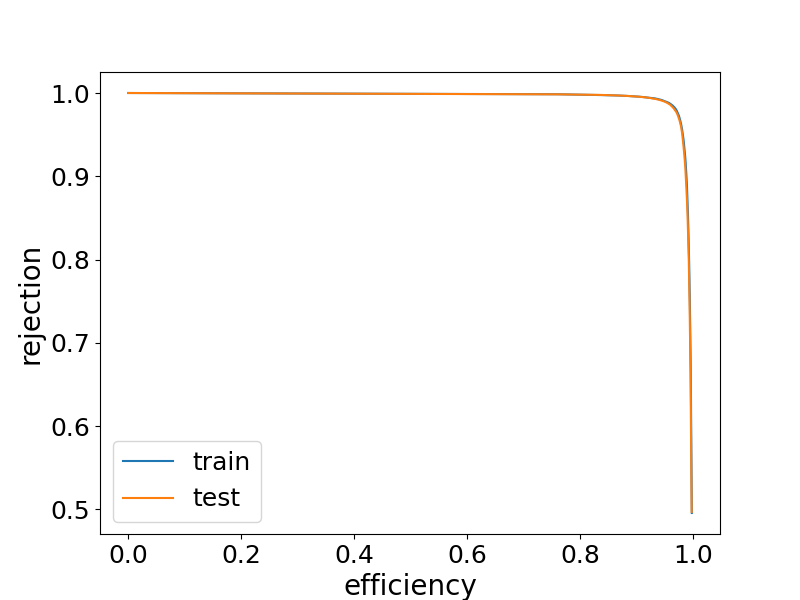
\includegraphics[height=6cm]{ROC_gen}
		%\label{fig:side:a}
	\end{minipage}
	\begin{minipage}[b]{0.5\linewidth}
		\centering 
		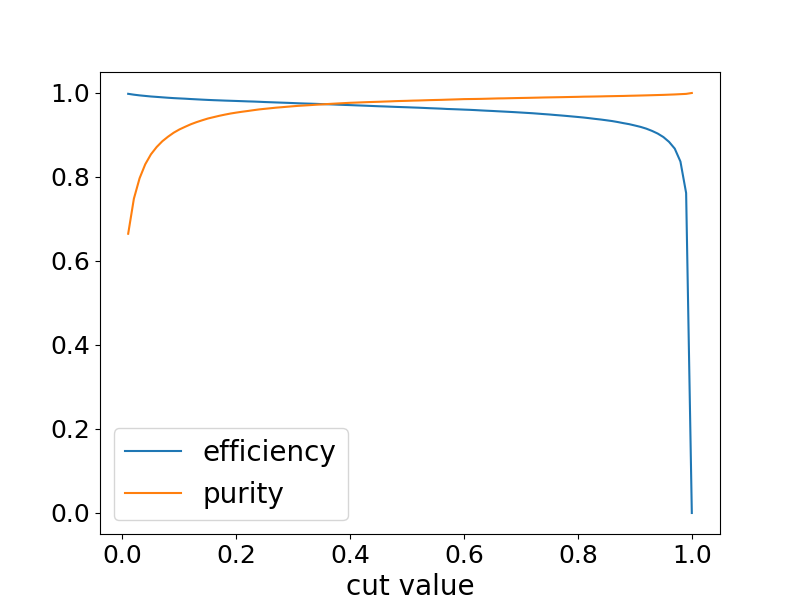
\includegraphics[height=6cm]{eff_gen}
		%\label{fig:side:b}
	\end{minipage}
	\caption{The left is ROC curve (blue for training and orange for testing) and the right is efficiency and purity (blue for efficiency and orange for purity) depending on cut of KsFinder output. Results are from generic MC sample.}
	\label{fig:gen_performance}
\end{figure}

\begin{comment}
\begin{figure}[H]
	\begin{minipage}[b]{0.5\linewidth}
		\centering 
		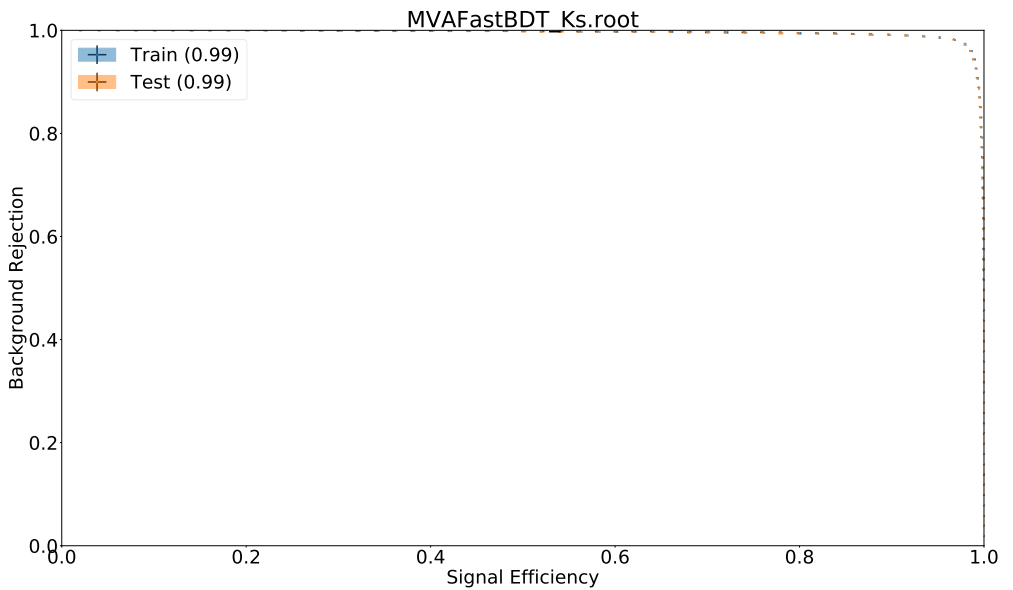
\includegraphics[height=4cm]{jpsi-jpsi}
		\label{fig:side:a}
	\end{minipage}
	\begin{minipage}[b]{0.5\linewidth}
		\centering 
		\includegraphics[height=4cm]{jpsi-jpsi-pur}
		\label{fig:side:b}
	\end{minipage}
	\caption{The left is ROC curve and the right is efficiency and purity depending on cut of classifier output. Results are from $B^0 \to J/\psi K_S^0$ generic decay sample.}
\end{figure}
\end{comment}

% 2021.02.08 mid
With increasing the efficiency, the cut on the output of KsFinder is getting loose. The background rejection only starts to drop when the efficiency exceeds about 90\% in both training and testing sample. To be noted, the curves are consistent in training and testing samples. 
While the ROC curve has shown the absence of noticeable over-fitting in classification, the detailed check can be made by comparing the distributions of classifier output on true and fake $K_S^0$ in training and testing samples. Therefore, the distribution of signal and background in training and testing sample with respect to the KsFinder output is plotted, where a distinctive separation for both signal MC and generic MC is shown and no over-training is found, as shown in Figure \ref{fig:ks_overtraining}.
\begin{figure}[H]
	\begin{subfigure}{1\linewidth}
		\centering
		\includegraphics[height=6cm]{over-3ks}
		\caption{Over-fitting check for signal MC sample.}
	\end{subfigure}
  	\vspace{0.3cm}

	\begin{subfigure}{1\linewidth}
		\centering
		\includegraphics[height=6cm]{over-gen}
		\caption{Over-fitting check for generic MC sample.}
	\end{subfigure}
\caption{The over-training check based on the comparison between training/testing data points in both signal and generic MC.}
\label{fig:ks_overtraining}
	\vspace{0.3cm}
	
%	\begin{subfigure}{1\linewidth}
%		\centering
%		\includegraphics[height=6cm]{over-jpsi}
%		\caption{Over-fitting check for  $B^0 \to J/\psi K_S^0$.}
%	\end{subfigure}
%\caption{Over-fitting check for classifiers.}
\end{figure}

The cut value for \textit{FBDT\_Ks} is determined by maximizing the ``Figure of Merit" (FOM), as shown Equation \ref{eq:fom}, where S and B is the number of true and fake $K_S^0$ after the cut, respectively. The FOM distribution depending on the cut value of FBDT\_Ks is shown in Figure \ref{fig:ks_fom}. The maximum FOM is achieved at FBDT\_Ks $= 0.74$ in signal MC, which is going to be used as the cut value to further reject fake $K_S^0$.

\begin{equation}\label{eq:fom}
	\text{FOM} = \frac{S}{\sqrt{S+B}}
\end{equation}

\begin{figure}[H]
	\centering
	\includegraphics[width=0.6\linewidth]{fom3ks}
	\caption{FOM of classifier output (FBDT\_Ks) in signal MC, the maximum value is achieved at 0.74 and the curve is almost flat between $0.5\sim 0.9$.}
	\label{fig:ks_fom}
\end{figure}

In the signal MC sample, the true $K_S^0$ fraction before applying KsFinder cut is 39\%, and 95.3\% of them are kept after the cut is applied. In the meantime, the fake $K_S^0$ fraction before applying the cut is 61\%, and 97.6\% of them are rejected after the cut is applied. The purity of the $K_S^0$ candidates is improved largely as shown in Figure \ref{fig:ks_cutused}.

\begin{figure}[htpb]
	\centering
	\includegraphics[width=0.7\linewidth]{kscutM}
	\caption{$K_S^0$ purity improvement with cut value of FBDT\_Ks at 0.74 applied. The blue solid line is true $K_S^0$ without KsFinder and green dashed line is the true $K_S^0$ with the cut applied. The orange solid line is fake $K_S^0$ without the cut and the red dashed line is fake $K_S^0$ with the cut. About 95.3\% of true $K_S^0$ are kept while 97.6\% of the fake ones are rejected by applying the cut.}
	\label{fig:ks_cutused}
\end{figure}

%2021/02/17 mids
\subsection{Data Validation for KsFinder}
The results from MC studies show an excellent performance of KsFinder. However, the validation of such a tool on the real experiment data is necessary. Since there's no MC truth on target variable in real data, the FastBDT method is based on variables in MC samples. If these variables shows close distribution among MC and data, the classification performance is expected to be similar.

In addtion, due to the fact that $K_S^0$ candidates are used for further reconstruction of $B^0$, the  mass and energy distributions may change after applying the cut, thus the validation that approves no clear bias on $B^0$'s variables that are used for signal extraction is also required. For comparison between MC and data, a small data sample from Belle II  experiment 7 and 8 is used. The integral luminosity at $\Upsilon(4S)$ resonance for this data sample is about 5.17 $\text{fb}^{-1}$. The MC sample is extracted from generic MC with equivalent luminosity.


 The Figure \ref{fig:ksvalid_1} shows the invariant mass and momentum distributions from data and MC samples, where the data and generic MC agree well. The uncertainties in data are calculated based on three times the Poisson standard deviation in each bin. The variable with the highest importance is the cosine angle between $K_S^0$ vertex and the direction of momentum, named as \textit{cosVertexMomentum}, of which distribution is shown in Figure \ref{fig:cosVex_dataMC}. In these comparison plots, the generic MC is shown in blue solid lines with no KsFinder cut used. Similarly, data without using cut of KsFinder are shown in yellow dots, which are closely distributed as the generic MC, indicating a good data MC consistency. Since the FastBDT algorithm relies on the probability density functions to seperate signal and backgrounds in each tree node, the similar distribution can lead to close classification power in data. The purple solid lines are presenting the true $K_S^0$ distribution in generic MC, while the red dots are the $K_S^0$ in data after using the cut value at 0.74. The reduced fraction of $K_S^0$ in data  is close to the signal MC. All distributions comparison between data and generic MC by using KsFinder cut are shown in Appendix B.

%\begin{comment}
\begin{figure}[htpb]
\begin{subfigure}{0.5\linewidth}
\includegraphics[page=2,width=1.1\linewidth]{dataVarsPlot_Ks}
\end{subfigure}
\begin{subfigure}{0.5\linewidth}
\includegraphics[page=7,width=1.1\linewidth]{dataVarsPlot_Ks}
\end{subfigure}
\bigskip
\begin{subfigure}{0.5\linewidth}
\includegraphics[page=8,width=1.1\linewidth]{dataVarsPlot_Ks}
\end{subfigure}
\begin{subfigure}{0.5\linewidth}
\includegraphics[page=9,width=1.1\linewidth]{dataVarsPlot_Ks}
\end{subfigure}
\caption{The distribution of invariant mass from charged pions and the momentum of $K_S^0$ in $x,y,z$ directions. The blue line is from all generic MC where the purple line is the true $K_S^0$ in it. The yellow dots are data with no KsFinder cut applied and the solid red dots are data after applying KsFinder cut at 0.74.}
\label{fig:ksvalid_1}
\end{figure}
%\end{comment}

 \begin{figure}[htpb]
	\centering
	\includegraphics[page=6,width=0.7\linewidth]{dataVarsPlot_Ks}
	\caption{The distribution of {cosVertexMomentum} in data and MC with/without KsFinder cut applied.}
	\label{fig:cosVex_dataMC}
\end{figure}

\subsection{Data and MC correction by KsFinder}
Implementing KsFinder cut on data may induce bias on the event numbers for $K_S^0$ because the training set of KsFinder is extracted from MC. To compensate such potential effect, a ratio as the data and MC correction is calculated based on the expected signal yield after using KsFinder. A maximum likelihood fit on invariant mass $M_{\pi^+\pi^-}$ for $K_S^0$ after applying cut value at 0.74 of KsFinder output is performed, where signal shape is modeled as a triple-Gaussian and background shape is modeled as a Chebyshev polynomial. The signal yield fraction is defined as Equation \ref{eq:S_ratio}.

\begin{equation}\label{eq:S_ratio}
	f_{K_S} = \frac{N_{sig}}{N_{tot}}
\end{equation}

where $N_{sig}$ is the signal number from the fit result and $N_{tot}$ is the total events number.
The fit is performed on both generic MC and data to obtained $f_{K_S} $, respectively.
The $\mathcal{R}_{K_S}$ is defined as the ratio of signal yield fraction  $f_{K_S} $ from MC and data as shown in Equation \ref{eq:R_Ks}. The ratio at cut value of 0.74 is $\mathcal{R}_{K_S} = 1.009\pm 0.011$ from the fit, as shown in Figure \ref{fig:Rfit}. Since the final state consists of three $K_S^0$, the expected ratio between MC and data for $B^0$ is expected to be the cube of $\mathcal{R}_{K_S}$, with the uncertainty propagated from the uncertainty of $\mathcal{R}_{K_S}$.  Therefore, the upper and lower limit for the correction ratio  $\mathcal{R}_{B^0}$ is expected to be $1.060$ and $0.994$. The result of $\mathcal{R}_{B^0}$ is $1.027 \pm 0.033$, which is close to 1 within its uncertainty. Hence, the correction $\mathcal{R}_{B^0}$ is not applied in signal extraction of $B^0$, but the uncertainty is taken into account as a possible systematic uncertainty term. 
 
\begin{equation}\label{eq:R_Ks}
\mathcal{R}_{K_S} = \frac{f_{K_S}^{MC}}{f_{K_S}^{data}}
\end{equation}

%\begin{equation}\label{eq:R_B}
%\mathcal{R}_{B^0} = \mathcal{R}_{K_S}^3
%\end{equation}

\begin{figure}[htpb]
	\begin{subfigure}{0.5\linewidth}
		\caption{Data,cut=0.74}
		\includegraphics[width=1\linewidth]{ksDatamva0.75.png}
	\end{subfigure}
\begin{subfigure}{0.5\linewidth}
	\caption{MC,cut=0.74}
	\includegraphics[width=1\linewidth]{ksMCmva0.75.png}
\end{subfigure}
\caption{The fit on invariant mass $M_{\pi^+\pi^-}$ where signal component is modeled as a triple-Gaussian and background component is modeled as a Chebyshev polynomial. The signal fraction is slight higher in MC compared to that in data.}
\label{fig:Rfit}
\end{figure}

\begin{comment}
\begin{subfigure}{0.5\linewidth}
\caption{Data,cut=0.9}
\includegraphics[width=1\linewidth]{ksDatamva0.9.png}
\end{subfigure}
\begin{subfigure}{0.5\linewidth}
\caption{MC,cut=0.9}
\includegraphics[width=1\linewidth]{ksMCmva0.9.png}
\end{subfigure}
\caption{Invariant mass fit of $K_S^0$ using cut at 0.2(loose) and 0.9(tight) to calculate $S_{data/MC}$.}
\end{figure}
\end{comment}

\begin{comment}
\subsection{Summary}
The development of Belle II $K_S^0$ classifier is enlighten by the experience from Belle. A comprehensive study of training observables from $K_S^0$ decay characteristics has been exploited. It takes the advantage of FastBDT algorithm to achieve a high fake rejection power. As a result, classifier is able to give a output which can be used as a cut to select good $K_S^0$ candidates with high purity. The classifier is validated with real experimental data as well. A primary data validation study of KsFinder is conducted with implementing correction on data and MC along with its contribution to $B^0$. The performance of KsFinder is in a good shape and no clear bias is found on the yield of the number of $K_S^0$. For the reconstruction of $B^0 \to K_S^0  K_S^0  K_S^0$, the development of KsFinder is critical to suppress large fraction of combination background from fake $K_S^0$.
\end{comment}

\chapter{$B^0$ reconstruction and event selection}

\begin{comment}
\section{Time Dependent \textit{CP} violation measurement}
The measurement of \textit{CP} violation in transitions of 
$B^0$ mesons to their common \textit{CP}
eigenstate $K_S^0 K_S^0 K_S^0$ requires the analysis of the time-dependent differential decay rates. The distribution of events based on the decay time difference $\Delta t$ and flavor is dependent on mixing induced and/or direct \textit{CP} parameters $\mathcal{S}$ and  $\mathcal{A}$. 

\begin{equation}
\mathcal{P}(\Delta t, q ) = 
\frac{e^{-|\Delta t|/\tau_{B^0}}}{4\tau_{B^0}}
\begin{Bmatrix}
1 + q \cdot 
\begin{bmatrix}
\mathcal{S}sin(\Delta M_d \Delta t) + 
\mathcal{A}cos(\Delta M_d \Delta t)
\end{bmatrix}
\end{Bmatrix}
\end{equation}

Here, same as discussed in Chapter 1, $\Delta M_d$ is the mass difference of two $B^0$ mass eigenstates, $\Delta t$ is the decay time difference of signal-side and tag-side $B^0$, namely $\Delta t = t_{CP} - t_{tag}$.  $\tau_B^0$ is the lifetime of $B^0$. And $q = + 1 (-1)$ is the indicator of flavor when tag-side meson is $B^0$ ($\bar{B^0}$). To a good aproximation using Eq(1.47), $\mathcal{A}$ is expected to be zero and $\mathcal{S} = -\text{sin}(2\phi_1)$, given the final states of $K_S^0 K_S^0 K_S^0$ corresponding to \textit{CP}-even ($n_f = + 1$). The previous result from Belle and Babar are shown in Fig 4-1. 

\begin{figure}
\centering 
\includegraphics[height=5cm]{belle_babar_result}
\caption{The results of Belle (2007) and Babar on -sin(2$\phi_1$)}
\end{figure}
\end{comment}


%\section{Data Sample and Event Selection}
\begin{comment}
The simulation data (MC) is taken from Belle II official MC campaign 13, named MC13. Both\textit{signal MC} and \textit{signal MC} are produced. In\textit{signal MC}, one of the $B^0$ from $\Upsilon(4S)$ decays into final states 3$K_S^0$ then into 6 charged pions, while the other $B^0$ decays generically using all possible channels. In \textit{signal MC},  $B^0$ from  $\Upsilon(4S)$ all decay generically using all possible channels.
The\textit{signal MC} sample is produced by EvtGen package with provided ``decay.dec" file that describes the required decay mode and branching fraction. As $K_S^0 \to \pi^0 \pi^0$ leads to large background with poor vertex quality, only the final states to 6 charged pions is used.
\end{comment}

As introduced in Section 2.9, the branching fraction of $B^0 \to K_S^0  K_S^0  K_S^0$ is $6.0 \times 10^{-6}$. The simulation sets the $\Upsilon(4S)$ as the mother particle then $\Upsilon(4S)$ decays into to two scalar $B^0$ mesons with mixing. $B^0 \to K_S^0  K_S^0  K_S^0$ decay process is simulated based on the possible phase-space the final state particles could obtain, where no $\it{CP}$ violation is implemented in the generator level, meaning that the input of $\mathcal{S}$(sin2$\phi_1$) and $\mathcal{A}$ are both zero. 
\section{$K_S^0$ Selection}
$K_S^0$ is first reconstructed by the cut-based method using two charged pions which contains a large fraction of fake candidates, as discussed in Chapter 3 and Table \ref{tab:kspipi_select}. In addition, a cut on $K_S^0$ is used considering momentum distribution of $B^0 \to K_S^0  K_S^0  K_S^0$, where the huge fake $K_S^0$ appear in low momentum region. Only the $K_S^0$ candidates with momentum larger than 0.05 GeV are selected, as shown in Figure \ref{fig:ks-p}. To further reduce the fake candidates in $K_S^0$ using \textit{KsFinder}, only $K_S^0$ with \textit{FBDT\_Ks} larger than 0.74 are kept.
\begin{figure}[ht]
	\centering
	\includegraphics[width=1\linewidth]{ks-p}
	\caption{The distribution of $K_S^0$ momentum. Candidates smaller than 0.05GeV/c are rejected.}
	\label{fig:ks-p}
\end{figure}
%The vertex fit of $K_S^0$ is performed using \textit{TreeFit}. 

\begin{comment}
If we check out the distribution of fitted invariant mass based on SVD hits number associated with daughter tracks as section 3.1 discussed, \textit{SVD00} $K_S^0$ shows a large dispersion from the central region of the distribution of invariant mass after vertex fit, while \textit{SVD11} $K_S^0$ shows a small dispersion as shown in Figure \ref{fig:invm1}. Therefore, considering the $K_S^0$ candidates with different SVD hits, see Figure \ref{fig:ks-r-svdxx} and Table \ref{tab:svdxx}, reflecting the different tracking quality of daughter $\pi^{\pm}$, the different cut on invariant mass M$_{\pi^+\pi^-}$ after vertex fit is applied depending on the SVD hits number of pion tracks. As shown in Figure \ref{fig:invm}, the sideband regions where fake $K_S^0$ is much higher than true $K_S^0$ are excluded. The cut windows are listed in Table \ref{tab:ks_invm}. This improves the reconstruction purity.
\end{comment}
 
 
 


\section{$B^0$  Reconstruction}
By combining three $K_S^0$ particles from selected $K_S^0$ candidates, $B^0$ candidates can be reconstructed. The beam-constraint mass $M_{bc}$ and energy difference $\Delta E$ are used to extract signal, as defined in Equation \ref{eq:mbc} and \ref{eq:dE}, respectively. 

\begin{equation}\label{eq:mbc}
M_{bc} = \sqrt{\frac{s}{4}-p^{*2}_B} 
\end{equation}
\begin{equation}\label{eq:dE}
\Delta E = E^*_B - \frac{\sqrt{s}}{2}
\end{equation}
For $M_{bc}$, $\sqrt{s}$ is defined as the invariant mass of the center-of-mass which is calculated from the beam energies and $p^*_B$ is the reconstructed $B$ momentum in the center-of-mass frame. For $\Delta E$, $E^*_B$ is the reconstructed energy in the center-of-mass frame. These two variables are quite useful for discriminating signal and background events for hadronic $B$ decay with fully reconstructed final states. In Belle II, the $B^0$ candidates with $M_{bc} > 5.2$ GeV and $|\Delta{E}| < 0.2$ GeV are required. 

The vertex information of the fully reconstructed $B^0 \to K_S^0  K_S^0  K_S^0$, called as $\it{CP}$-side, is obtained by the vertex fit using \textit{TreeFit} and the $\chi^2$ probability of the fit is calculated.  Only $B^0$ candidates with converged vertex fit results are kept by a very loose cut of  $P(\chi^2)> 0.001$. On the other hand, the $\it{CP}$ violation measurement does not require the certain decay mode of the other $B^0$ meson in the Rest-Of-Event which includes all particles except for the ones used on the $\it{CP}$-side reconstruction. The $B$ meson in the Rest-Of-Event is called as tag-side $B$ since this $B$ is used to tag the flavor of $\it{CP}$-side $B$. Thus, no full $B^0$ reconstruction on the tag-side is performed, meaning that the vertex information can not be obtained by the specific final states. Considering this strategy, the vertex fit on the tag-side is done by \textit{KFit} that only takes advantage of well-reconstructed charged particle tracks. The vertex on the tag-side are required to be located inside the standard PXD region, despite that PXD is not fully installed yet. In future, such requirement is subjected to be modified by the PXD hits requirements. 
 
 After performing the vertex fit for both $\it{CP}$-side and tag-side, we check the potential impact of applying \textit{KsFinder} on the reconstructed vertex positions, as well as the impact on the $M_{bc}$ and $\Delta E$. It is necessary for mainly two reasons. First, the \textit{KsFinder} might change the original distributions of $M_{bc}$ and $\Delta E$ of $B^0$ candidates, which are used for the signal extraction. The signal extraction will provide the signal fraction information that is used during the $\it{CP}$ parameter measurement. Second, the \textit{KsFinder} might introduce the bias on the distribution of the vertex positions of $B^0$. The $K_S^0$ candidates with less SVD hits on their daughter pion tracks usually have poorer reconstruction quality and more likely to be rejected as fake candidates. Therefore, we check the distribution of $M_{bc}$ and $\Delta E$ before and after the applying \textit{KsFinder}, as well as the distribution of vertex positions on the $z$-axis. The details about the comparison can be found in the Appendix E. In conclusion, applying \textit{KsFinder} has a negligible impact on $M_{bc}$, $\Delta E$ and the vertex positions on the $z$-axis. The contribution of \textit{KsFinder} as a possible systematic uncertainty source mainly comes from the different data and MC responses of the $K_S^0$ classification, as discussed in the Section 3.2.7. 
 
When multiple $B^0$ candidates are obtained in a single event, the best candidates selection (BCS) is performed by ranking their $\chi^2$ of the $\it{CP}$-side vertex fit. Since the BCS is based on the $\chi^2$ that might introduce bias in the vertex positions for $\it{CP}$ fit, we check the distribution of the vertex $\chi^2$, as shown in Figure \ref{fig:b0dist} top left where the data and \textit{generic MC} present a good consistence within $1\sigma$ on average. The distribution of the candidate number per event without BCS is shown in top right of Figure \ref{fig:b0dist} as well, showing an agreement between data and \textit{generic MC} within around 1$\sigma$. The distribution of the candidate number per event from the \textit{signal MC} is also in the bottom left of Figure \ref{fig:b0dist}. The 2D distribution of $M_{bc}$ and $\Delta E$ from $B^0 \to K_S^0  K_S^0  K_S^0$ \textit{signal MC} is shown in Figure \ref{fig:b0dist}  bottom right, where the correlation factor is about 15\% between two observables. 
 
\begin{figure}[htpb]
	\begin{minipage}[b]{0.5\linewidth}
		\centering 
		\includegraphics[width=1\linewidth, height=6cm]{figures/best_treeFitChi2_noBCS}
		
	\end{minipage}
	\begin{minipage}[b]{0.5\linewidth}
		\centering 
		\includegraphics[width=1\linewidth, height=6cm]{figures/best_ncands_noBCS}
		
	\end{minipage}
	\begin{minipage}[b]{0.5\linewidth}
		\centering 
		\includegraphics[width=1\linewidth, height=6cm]{figures/best_ncands_sig}
		
	\end{minipage}
	\begin{minipage}[b]{0.5\linewidth}
		\centering 
		\includegraphics[width=1\linewidth, height=6cm]{figures/hist_sig_MC_Mbc_dE}
		
	\end{minipage}
	
	\caption{Top left is the $\chi^2$ for data and \textit{generic MC} before BCS. Top Right is the $B^0$ candidates per event in data and \textit{generic MC} before the BCS. Bottom left is the number of $B^0$ candidates per event from \textit{signal MC}. Bottom right is the 2D $M_{bc}$ and $\Delta E$ distribution from \textit{signal MC}.}
	\label{fig:b0dist}
\end{figure}
% move to after CS
\section{Continuum Suppression}
The generic decay of $\Upsilon$(4S) produces neutral and charged $B$ mesons, as well as other flavor mesons $q\bar{q}$. Since the branching fraction of $B^0 \to K_S^0  K_S^0  K_S^0$ is relatively low, the $B^0$ candidates after the reconstruction contain a large fraction of fake ones if no special reduction on $q\bar{q}$ is applied. 
The $q\bar{q}$ background events are distributed as a continuum-like shape in the distribution of $M_{bc}$ and $\Delta E$. This calls a demand to distinguish $B\bar{B}$ decay events from $q\bar{q}$ events, which is called as continuum suppression (CS). The rejection is essential because it is the dominated background in this analysis. The most useful information to reject $q\bar{q}$ events is to use the event shape information. In a $B\bar{B}$ event, two mesons are produced almost at rest in the CMS frame since the resonance state $\Upsilon(4S)$ is just slightly lighter than the beam energy. As a result, decay products are emitted more isotropically compared to continuum background events which are more jet-like, back-to-back flying out from the interaction region. The ARGUS and CLEO collaboration developed a set of variables to suppress the continuum background~\cite{Bevan_2014}, which has also been implemented into BASF2 framework. The two major sets of variables are the CLEO cone momentum variables and the modified Super Fox-wolfram momentum variables.

CLEO cone momentum can be presented as Equation \ref{eq:ln}, where $ p_i $ is momentum of i-th particle in the Rest-Of-Event (ROE). The particles used in a reconstructed $\it{CP}$-side $B^0$ are therefore excluded. The $\theta_i$ is an angle between $\vec{p_i}$ and the momentum thrust axis of the reconstructed $\it{CP}$-side \textit{B} meson. The angle is divided into the binned intervals in nine cones of 10 degrees around the thrust.  The $L_n$ stands for the combination that includes particles in a certain cone. The demonstration of the intervals of the CLEO cone is shown in Figure \ref{fig:cleocone}. The distribution of the first CLEO cone momentum variable in the signal and continuum background events is shown in Figure \ref{fig:cleo1}.
\begin{equation}\label{eq:ln}
L_n = \sum_{i\in ROE}^{} p_i \times |\text{cos}\theta_i|
\end{equation}

\begin{figure}[htpb]
\centering
\includegraphics[width=0.6\linewidth]{cleocone}
\caption{A graphical illustration of the CLEO cone. The $h^+$ and $h^{'-}$ present the hadronic tracks from a $B$ decay. The first three cones are drawn~\cite{Bevan_2014}. The nine CLEO cone momentum can be calculated using the particles in each cone. }
\label{fig:cleocone}
\end{figure}
\begin{figure}[htpb]
	\centering
	\includegraphics[width=0.7\linewidth]{cleo1.png}
	\caption{The distribution of the first CLEO cone momentum variable in the signal and continuum background events.}
	\label{fig:cleo1}
\end{figure}

The modified Super Fox-wolfram momentum (KSFW momentum) can be defined as shown in Equation \ref{eq:ksfw}.
\begin{equation}\label{eq:ksfw}
KSFW = \sum_{l=0}^{4}( R_l^{so} + R_l^{oo}) + \gamma \sum_{n=1}^{N_t}|P(t)_n|
\end{equation} 
The $R_l^{so}$ and $R_l^{oo}$ are the functions which depend on both $\it{CP}$ and tag-side particles. Their values are also affected by whether $l$ is even or odd. The $P(t)_n$ is the scalar sum of the transverse momentum of
each particle multiplied by a free parameter $\gamma$ and $N_t$ is
the total number of particles. The detailed  definition for each KSFW momentum is described in Ref.~\cite{Bevan_2014}. As an example, the distribution of one of the KSFW momentum variables is shown in Figure \ref{fig:ksfw4}.

\begin{figure}[htpb]
	\centering
	\includegraphics[width=0.7\linewidth]{ksfw4.png}
	\caption{The distribution of the variable \textit{KSFWV9} in the signal and continuum background events.}
	\label{fig:ksfw4}
\end{figure}

\begin{comment}

where the first term is shown in Equation \ref{eq:rlso}.
\begin{equation}\label{eq:rlso}
R_l^{so} = \frac{\alpha_{cl}H_{cl}^{so} +
				\alpha_{nl}H_{nl}^{so}+
			\alpha_{ml}H_{ml}^{so}}{E^*_{beam}-\Delta E}
\end{equation}

when l is odd in Equation \ref{eq:rlso}: 
\begin{equation}
	H_{nl}^{so}=H_{ml}^{so}=0
\end{equation}
and $H_{cl}^{SO}$ is defined as shown in Equation \ref{eq:hclso}: 
\begin{equation}\label{eq:hclso}
	H_{cl}^{so} = \sum_i \sum_{jx}Q_i Q_{jx}|p_{jx}|P_l(cos\theta_{i,jx})
\end{equation}
\textit{i} runs over \textit{B} daughter particles and \textit{jx} for other particles in ROE. \textit{Q} is charge and $p_{jx}$ is momentum for each particle. $P_l(cos\theta_{i,jx})$ is the \textit{i}-th order Legendre polynomial of cosine of \textit{i} and \textit{jx}-th particles.
On the other hand, for \textit{l} is even, $H_{xl}^{SO}$ can be written in Equation \ref{eq:hxlso}.
\begin{equation}\label{eq:hxlso}
	H_{xl}^{so}=\sum_i \sum_{jx}|p_{jx}|P_l(cos\theta_{i,jx})
\end{equation}
The second term in Equation \ref{eq:ksfw}, when \textit{l} is odd, can be defined as Equation \ref{eq:roo}.
\begin{equation}\label{eq:roo}
	R^{oo}_l = \sum_j \sum_k \beta_l Q_j Q_k |p_j||p_k|P_l(cos\theta_j,k)
\end{equation}
\textit{j} and \textit{k} runs over ROE particles and others are same as Equation \ref{eq:hclso}.
For an even \textit{l}: 
\begin{equation}
	R^{oo}_l = \sum_j \sum_k \beta_l |p_j||p_k|P_l(cos\theta_j,k)
\end{equation}
$\beta$ is Fisher coefficients to be determined. 
\end{comment}


\begin{comment}
Besides, two other variables, cos$\theta_B$ and $\Delta Z$, are also quite useful for CS, where the former is the cosine of the angle between $B$ momentum and the beam direction and the latter is the distance between $\it{CP}$ and tag-side $B$ vertices along the beam direction. Both of them are calculated in the CMS frame.
Using these two variables and KSFW momentum, we can form the possibility density functions in the signal and continuum background events. The product of the probability density values for each event is presented as a likelihood of being signal or background, as shown in the Equation \ref{eq:Lsb}. Then we can calculate a ratio $\mathcal{R}$ as Equation \ref{eq:Rcs} shows. It is clear that for a event with very high probability of being a signal, $\mathcal{R}$ is close to 1.

\begin{equation}\label{eq:Lsb}
L_{S/B} = P(KSFW)_{S/B} \times P(cos\theta_B)_{S/B} \times P(\Delta Z)_{S/B}
\end{equation}

\begin{equation}\label{eq:Rcs}
\mathcal{R} = \frac{L_S}{L_S+L_B}
\end{equation}

\end{comment}

In addition to the CLEO cone and KSFW momentum, a few other variables that are related to the event-shape topology are also used in the Belle II CS framework in order to obtain a better continuum background rejection performance. 
This includes $R_2$, $cosTBz$, $cosTBTO$, $thrustOm$, and $thrustBm$.
$R_2$ is defined as the normalized second Fox-Wolfram moment ratio, which is widely used in the decay shape studies. The distribution of $R_2$ is shown in Figure \ref{fig:R2}.
The $cosTBTO$ is cosine of angle between thrust axis of the $\it{CP}$-side $B$ meson and thrust axis of Rest-Of-Event.
The $cosTBz$ is cosine of angle between thrust axis of the $\it{CP}$-side $B$ meson and $z$-axis.
The $thrustOm$ and $thrustBm$ are the magnitude of the $\it{CP}$-side $B$ thrust axis and Rest-Of-Event thrust axis, respectively. 


 


\begin{figure}[htpb]
	\centering
	\includegraphics[width=0.7\linewidth]{r2}
	\caption{$R_2$ is the ratio of the second to the zeroth KSFW momentum in Equation \ref{eq:ksfw} of which the distribution in \textit{signal MC} sample which serves as the highest weight as a variable in discriminating the continuum events, having a quite different distribution between signal and background.}
	\label{fig:R2}
\end{figure}

For the Belle II CS strategy, the default method is to use the above variables as an input for a FastBDT classifier to discriminating the signal and continuum background. For the specific decay mode $B^0 \to K_S^0  K_S^0  K_S^0$, the training and testing samples prepared from \textit{signal MC} and \textit{generic MC} are used. The target variable of the training is the continuum event truth named $NotContinuumEvent$, where for signal~(continuum background) the value is 1~(0).  The same event-reconstruction procedure for $B^0$ is applied for both MC samples. Events passing the selection using $M_{bc}$ and $\Delta E$ are used for training the CS classifier. The fraction of signal and background is set to 1:1. The output of CS classifier is called \textit{FBDT\_CS}.  We determine the cut value at 0.66 based on the maximum of \textit{FOM} curve, as shown in Figure \ref{fig:cs_fom}. The input variables are listed in Table \ref{tab:cs_abr} with their abbreviations in the training. After the training, the importance of the input variables can be evaluated, shown as Figure \ref{tab:cs_imp-h}.

\begin{figure}[htpb]
	\centering
	\includegraphics[width=0.6\linewidth]{cs-fom}
	\caption{\textit{FOM} depending on the cut value of continuum classifier output, cut value at 0.66 is used for continuum suppression. }
	\label{fig:cs_fom}
\end{figure}

\begin{figure}[htpb]
	\centering 
	\caption{The importance rank of the input variables for the Belle II CS framework.}
	\label{tab:cs_imp-h}
	\includegraphics[width=0.9\linewidth]{cs-imp-h}
\end{figure}

The correlation between these training variables are shown in Figure \ref{fig:cs_cor} which are varied between signal and continuum background events. The ROC curve and the efficiency/purity using the testing samples with respect to the classifier output are shown in Figure \ref{fig:cs_roc}, yielding a close performance to the training.
\begin{table}[htpb]
	\begin{minipage}[t]{1\linewidth}
		\centering
		\caption{Input variables and the abbreviations in the continuum suppression framework of BASF2.}
		\label{tab:cs_abr}
		\begin{tabular}{c|c}
			\hline
			Observables &  Abbreviations\\
			\hline
			CleoConeCS(9) &  CleoC1 \\
			KSFWVariables(hoo1,) & KSFWV1 \\
			CleoConeCS(7) & CleoC2\\
			CleoConeCS(5) & CleoC3\\
			KSFWVariables(hso22) & KSFWV2\\
			KSFWVariables(hoo3) & KSFWV3\\
			CleoConeCS(4) & CleoC4 \\
			KSFWVariables(hoo4,) &  KSFWV4\\
			CleoConeCS(3) & CleoC5 \\
			CleoConeCS(6) & CleoC6\\
			CleoConeCS(8) & CleoC7\\
			KSFWVariables(hso14) &   KSFWV5\\
			KSFWVariables(hso00) & KSFWV6\\
			KSFWVariables(et) & KSFWV7\\
			KSFWVariables(hso24) & KSFWV8\\
			KSFWVariables(hso04) & KSFWV9\\
			KSFWVariables(hso20) & KSFWV10 \\
			KSFWVariables(mm2)  & KSFWV11\\
			KSFWVariables(hoo2) &  KSFWV12\\
			thrustOm & thrus1 \\
			cosTBz & cosTB1\\
			CleoConeCS(1) & CleoC8 \\
			CleoConeCS(2) & CleoC9 \\
			KSFWVariables(hso02) &  KSFWV13\\
			KSFWVariables(hoo0) &  KSFWV14 \\
			KSFWVariables(hso12) &  KSFWV15\\
			KSFWVariables(hso10) & KSFWV16\\
			cosTBTO & cosTB2\\
			thrustBm & thrus2\\
			R2 & R2\\
			\hline
		\end{tabular}
	\end{minipage}
\end{table}

\begin{figure}[htpb]
	\begin{minipage}[b]{0.5\linewidth}
		\centering 
		\includegraphics[width=1\linewidth]{figures/corr_cs_kine_sig}	
	\end{minipage}
\begin{minipage}[b]{0.5\linewidth}
	\centering 
	\includegraphics[width=1\linewidth]{figures/corr_cs_kine_bkg}	
\end{minipage}
	\caption{The correlation in variables for continuum suppression. The left is for signal and the right is for background.}
	\label{fig:cs_cor}
\end{figure}
\begin{figure}[htpb]
	\begin{minipage}[b]{0.5\linewidth}
		\centering 
		\includegraphics[height=6cm]{figures/ROC_CS}	
	\end{minipage}
	\begin{minipage}[b]{0.5\linewidth}
		\centering 
		\includegraphics[height=6cm]{figures/eff_CS}	
	\end{minipage}
\caption{The left is the ROC curve (blue for training and orange for testing)
	and the right is the efficiency~(blue) and purity~(orange) regarding the classifier output \textit{FBDT\_CS}.}
	\label{fig:cs_roc}
\end{figure}

The overtraining check is made by comparing the distribution of signal and background depending on the classifier output in both training and testing samples. The testing sample shows about 1\% lower in each bin for both signal and background events, which is within the acceptable range.  
\begin{figure}[htpb]
	\centering
	\includegraphics[width=1\linewidth]{cs-overtrain}
	\caption{Over training check of continuum classifier, where a very small difference in training and testing (1\%) is shown.}
\end{figure}


\subsection{Event selection summary}
The summary of Event selections is listed in Table \ref{tab:b0select}, including the application of \textit{KsFinder} (by \textit{FBDT\_Ks}) and continuum suppression (by \textit{FBDT\_CS}).
\begin{table}[htpb]
	\centering 
	\begin{tabular}{c|c|c|c|c|c|c|c} 
		\hline
		$B^0$  & $M_{bc}$(GeV/$c^2$)& $\Delta E$(GeV) & $P(\chi^2)$ & \textit{Rank} & \textit{FBDT\_CS} & \textit{FBDT\_Ks}\\
		\hline
		Criteria & $> 5.20$ \& $< 5.29$  &  $ |\Delta E|< 0.2$ & $> 0.001$  & $=1$ & $>0.66$ & $>0.74$\\
		\hline
	\end{tabular}
	\caption{$B^0$ selection criteria, $P(\chi^2)$ is from $B^0$ $\it{CP}$-side vertex fit and \textit{Rank} is from the BCS}
	\label{tab:b0select}
\end{table}

Combined with the previous paragraph, the reconstruction performance of $B^0$ is summarized in Table \ref{tab:b0stats}. The efficiency, purity, fraction of multiplicity events and best candidates fraction of $B^0$ are slightly improved in the Belle II compared to the ones referenced from Belle~\cite{kang2020measurement}.
\begin{table}[H]
	\centering
	\begin{tabular}{c|c|c|c|c}
		\hline
		event selection & efficiency & purity  & $f_{MB}$  & BCS \\
		\hline
		\hline
		Belle Standard & 35\%(33\%) & 96\%(99\%) & 6\%(6\%) & 83\%(96\%)\\
		\hline 
		Belle II (\textit{BG1}) & 36\%(34\%) & 96\%(98\%) & 4\%(4\%) & 95\%(96\%)\\
		\hline
		Belle II (\textit{BG0}) & 40\%(36\%) & 96\%(99\%) & 3\%(3\%) & 97\%(97\%)\\
		\hline
	\end{tabular}
	\caption{The efficiency is defined by the fraction of best candidates among the MC input number. Purity is the fraction of true $B^0$ in best candidates. $f_{MB}$ stands for multiple $B^0$ events fraction in true signal events. BCS is the fraction of best candidates being a true signal. All values in the parenthesis are calculated in $| M_{bc} |- 5.28 < 0.1$ and $|\Delta E| < 0.1$, called as ``signal region" where efficiency is lower but purity is higher, compared to the full range of $M_{bc}$ and $\Delta E$ in Table \ref{tab:b0select}. \textit{BG1} and \textit{BG0} indicate that the corresponding values are obtained using \textit{signal MC} with or without the beam background respectively, which the \textit{BG0} sample yields a slightly better reconstruction performance. }
	\label{tab:b0stats}
\end{table}


% summary of $B^0$ stats goes here
\section{Resonance Background}

The $\it{CP}$ eigenvalue of $B^0 \to K_S^0  K_S^0  K_S^0$ is $\eta_f = +1$ if it is a loop-level $b\to s$ transition, called $\it{CP}$-even. However, the charmonium resonances from $b \to c$ tree-level transition can give an odd $\textit{CP}$ eigenvalue ($\eta_f = -1$) while producing the same final states as $B^0 \to K_S^0  K_S^0  K_S^0$.  This would cause the contamination to the $\it{CP}$ measurement due to the fact that $\mathcal{S} = -\eta_f\text{sin}(2\phi_1)$. The loop-level $\it{CP}$-even processes are demonstrated in the left and middle diagrams of Figure \ref{fig:3ksfey}, including the phase-space based decay and resonance decays. Both are considered as the signal events. The tree-level $\it{CP}$-odd process is shown in the right diagram of Figure \ref{fig:3ksfey}, which is usually referred as the resonance background and can be rejected by applying cut on the invariant mass of two $K_S^0$ around the possible charmonium resonant states. Therefore, to check wether a resonance decay is a signal or background event, a list of possible $B^0 \to X(\to K^0_S K^0_S) K^0_S$ processes are considered. For the resonance decays of signal events, $X$ could be $f_2(1270)$, $f_0(1500)$, $f_{2}^{'}(1525)$, $f_0(980)$, $f_0(1710)$ and $f_2(2010)$. For the resonance background, \textit{X} could be $D^0$, $\eta$, $J/\psi$, $\psi(2S)$,  $\chi_{c0}$, $\chi_{c1}$, and $\chi_{c2}$.
The branching fraction of these decay modes in the PDG and the Belle II decay profile are both checked and compared, where some of them are not yet measured or not implemented in the Belle II simulation. Thus it is hard to precisely evaluate all the contributions from these decay modes. The expected contributions are calculated by using $2.14\times 10^8 B\bar{B}$ pairs corresponding to 400 fb$^{-1}$ as shown in the Table \ref{tab:f_res}. The main contribution from the resonance background is $B^0\to \chi_{c0} K^0_S$ and the main contribution from the resonant signal is $B^0\to f_0(980)K^0_S$. Given the very limited statistics of data accumulation we used in this analysis, the contribution of $\it{CP}$-odd resonance background should be smaller than one event. Besides, the comparison of two $K_S^0$ invariant mass using data and \textit{generic MC} is performed, while the small number of reconstructed events in data can not provide reasonable information on the distribution, see Appendix C. Hence, currently no veto of two $K_S^0$ invariant mass is applied to avoid potential bias in this low statistics scenario. In the future with more data collected, the veto will be first checked by the proper comparison between data and MC, then applied according to mass of the main contributive resonance states.
\begin{sidewaystable}
	\caption{Expected yield for signal and background resonances $2.14\times 10^8 B\bar{B}$ in \textit{generic MC}. The branching fraction of $B\to X K_S$ and $X \to 2K_S$ are listed from both the PDG values and the values used in Belle II generic decay profile. The number of events from $\it{CP}$-odd resonance background is expected to be smaller than one at current luminosity 62.8 fb$^{-1}$.}
	\label{tab:f_res}
	\centering
	\begin{tabular}{|c|c|c|c|c|c|c|}
		\hline
		Resonances & Br($B \to X K_S$)PDG  & Br($X \to2K_S$) & Br($B \to X K_S$)Dec. & Br($X \to2K_S$)Dec. & $B\bar{B}$ pairs & Expected yields \\
		\hline
		$D^0 K_S$ & $2.6 \times 10^{-5}$ & $1.7\times 10^{-4}$ & $2.6 \times 10^{-5}$ & $1.8\times 10^{-4}$ & $2.14\times 10^8$ & 0.134 \\
		\hline
		$\eta K_S$ & $3.45\times 10^{-4}$ & $<3.1\times 10^{-4}$ & $4\times 10^{-4}$ & No Value & $2.14\times 10^8$ & No Value  \\
		\hline
		$J/\psi K_S$ & $4.35\times 10^{-4}$ & $<1.4\times 10^{-8}$ & $4.35\times 10^{-4}$ & 0 & $2.14\times 10^8$ & 0 \\
		\hline
		$\psi(2S)K_S$ & $2.9\times 10^{-4}$ & $<4.6\times 10^{-6}$ & $2.9\times 10^{-4}$ & 0 & $2.14\times 10^8$ & 0 \\
		\hline
		$\chi_{c0}K_S$ & $7.3\times 10^{-5}$ & $3.16\times 10^{-3}$ & $7.35\times 10^{-5}$ & $3.1\times 10^{-3}$ & $2.14\times 10^8$ & 6.21 \\
		\hline
		$\chi_{c1}K_S$ & $1.96\times 10^{-4}$ & $6\times 10^{-5}$ & $1.96\times 10^{-4}$ & $1\times 10^{-5}$ & $2.14\times 10^8$ & 0.05 \\
		\hline
		$\chi_{c2}K_S$ & $7.5\times 10^{-6}$ & $2.6\times 10^{-4}$ & $7.5\times 10^{-6}$ & $5.5\times 10^{}-4$ & $2.14\times 10^8$ & 0.11 \\
		\hline
		$f_2(1270)K_S$ & $1.35\times 10^{-6}$ & $1.15\times 10^{-2}$ & $1.35\times 10^{-6}$ & $1.15\times 10^{-2}$ & $2.14\times 10^8$ & 0.42 \\
		\hline
		$f_{2}^{'}(1525)K_S$ & $1.5\times 10^{-7} $ & $2.22\times 10^{-2}$ & No value & 0.22 & $2.14\times 10^8$ & No Value \\
		\hline
		$f_2(2010)K_S$ & $5\times 10^{-7}$ & No Value  & No Value  & No Value  & $2.14\times 10^8$ & No Value \\
		\hline
		$f_0(980)K_S$ & $2.7\times 10^{-6}$ & No Value & $2.75\times 10^{-6}$ & No Value & $2.14\times 10^8$ & 43.3 \\
		\hline
		$f_0(1710)K_S$ & $5\times 10^{-7}$ & No Value  & No Value  & No Value  & $2.14\times 10^8$ & No Value \\
		\hline
		$f_0(1500)K_S$ & $6.5\times 10^{-5}$ & 0.022 & No Value & 0.022 & $2.14\times 10^8$ & No Value \\
		\hline
		Total  & - & - & - & - & - & $\simeq$50 \\
		\hline
	\end{tabular}
\end{sidewaystable}


% 2021.02.10 mid
\section{$B\bar{B}$ background}
Another possible contribution of background comes from $B\bar{B}$ events. Both neutral and charged $B\bar{B}$ pairs could produce the background events. Compared to the event number from the continuum background, the number of $B\bar{B}$ background is much fewer. By counting the background event number from $B\bar{B}$ and $q\bar{q}$ using \textit{generic MC}, the fraction of $B\bar{B}$ takes about 3\% among all background events, and no special treatment is implemented. 

\section{Signal Extraction}
The event selections defined in Table \ref{tab:b0select} is applied to \textit{signal MC}, \textit{generic MC} and experiment data for extracting signal events. The integral luminosity in \textit{generic MC} is 1 ab$^{-1}$ and experiment data used in this analysis is 62.8 fb$^{-1}$ from the latest official processing. The distribution of $M_{bc}$ and $\Delta E$ from \textit{generic MC} are shown in Figure \ref{fig:2Dgenstack} which contains about 21 signal events, 44 continuum background events and 2 $B\bar{B}$ background events if it is normalized to the data luminosity. The distribution of $M_{bc}$ and $\Delta E$ from data are also shown in Figure \ref{fig:2Ddatastack}, where 119 events are observed.

\begin{figure}[htpb]
	\begin{minipage}[b]{0.5\linewidth}
		\centering 
		\includegraphics[width=1\linewidth]{figures/hist_stacked_generic_mbc_oldksfinder}
	\end{minipage}
	\begin{minipage}[b]{0.5\linewidth}
		\centering 
		\includegraphics[width=1\linewidth]{figures/hist_stacked_generic_dE_oldksfinder}
	\end{minipage}
	\caption{The distribution  of $M_{bc}$ and $\Delta E$ for selected events from \textit{generic MC}, where each background components are stacked with signal normalized to 62.8 fb$^{-1}$. The blue component is the continuum background. The green and the black are the background from charged and neutral $B\bar{B}$ events. The red component is the signal component by checking MC truth matching. }
	\label{fig:2Dgenstack}
\end{figure}
\begin{figure}[htpb]
	\begin{minipage}[b]{0.5\linewidth}
		\centering 
		\includegraphics[width=1\linewidth]{figures/hist_stacked_data_mbc_}
		\label{}
	\end{minipage}
	\begin{minipage}[b]{0.5\linewidth}
		\centering 
		\includegraphics[width=1\linewidth]{figures/hist_stacked_data_dE_}
		\label{}
	\end{minipage}
	\caption{The distribution  of $M_{bc}$ and $\Delta E$ for selected events from the experiment data of 62.8 fb$^{-1}$.}
	\label{fig:2Ddatastack}
\end{figure}

The unbinned maximum likelihood fit using RooFit is performed to extract the signal. The 2D fit using both $M_{bc}$ and $\Delta{E}$ are done by taking the probability density function:
\begin{equation}\label{eq:pmbcde}
\mathcal{P}(M_{bc},\Delta{E}) = 
f_{sig}\times \mathcal{P}_{sig}^{M_{bc}}\times\mathcal{P}_{sig}^{\Delta{E}}
+ 
(1-f_{sig})\mathcal{P}_{bkg}^{M_{bc}}\times\mathcal{P}_{bkg}^{\Delta{E}} ~,
\end{equation}
where $\mathcal{P}_{sig}^{M_{bc}}$ and $\mathcal{P}_{sig}^{\Delta{E}}$ are the probability density function (P.D.F) for the distributions of $M_{bc}$ and $\Delta E$. The $f_{sig}$ is the fraction of signal events. We use the single Gaussian function as $\mathcal{P}_{sig}^{M_{bc}}$  in the distribution of $M_{bc}$ and triple Gaussian functions as $\mathcal{P}_{sig}^{\Delta{E}}$  in the distribution of $\Delta E$ to model the signal component. 

On the other hand, the dominated background comes from the continuum events, which is modeled as the Argus function~\cite{albrecht1990search} in the distribution of $M_{bc}$:
\begin{equation}\label{eq:Argus}
\mathcal{P}_{bkg}^{M_{bc}}(x;c,\chi)=\frac{\chi^3}{\sqrt{2\pi}\Psi(\chi)}\cdot
\frac{x}{c^2}\sqrt{1-\frac{x^2}{c^2}}\cdot
\exp \begin{Bmatrix}
-\frac{1}{2}\chi^2(1-\frac{x^2}{c^2}) ~
\end{Bmatrix}~,
\end{equation}
where $x$ presenting $M_{bc}$ is defined in $0<x<c$ with a preset mass threshold at $c = 5.29$ GeV. The $\chi$ is a parameter of the distribution. The $\Psi(\chi)=\Phi(\chi)-\chi\phi(\chi)-\frac{1}{2}$ where $\Phi(\chi)$ and $\phi(\chi)$ are cumulative distribution and probability density function of the standard normal distribution, respectively. The $\Delta E$ distribution of continuum events is modeled by the first order Chebyshev polynomial function. The scattered distribution of $M_{bc}$ and $\Delta E$ in the 2D plane is shown in Figure \ref{fig:hist_2Dplot}.

\begin{figure}[htbp]
		\centering 
		\includegraphics[width=0.6\linewidth]{hist_2Dplot}
		%\label{fig:side:b}
	\caption{The 2D distribution of $M_{bc}$ and $\Delta E$ in the 62.8 fb$^{-1}$ experiment data.}
	\label{fig:hist_2Dplot}
\end{figure}

The unbinned maximum likelihood fit is first performed to obtain the parameters for signal functions using \textit{signal MC}, and then fixed them as the constants latter for 2D fit. The fit results on \textit{signal MC} are shown in Figure \ref{fig:mbcde1D}. The continuum background is fitted by using $q\bar{q}$ events from \textit{generic MC} to determine the shapes then fix them as the constants latter for 2D fit. The fit results on \textit{$q\bar{q}$} events are shown in Figure \ref{fig:bkgmbcde}.
 \begin{figure}[htbp]
 	\begin{minipage}[b]{0.5\linewidth}
 		\centering 
 		\includegraphics[height=6cm]{mbc_sig_fit}
 		%\label{fig:side:a}
 	\end{minipage}
 	\begin{minipage}[b]{0.5\linewidth}
 		\centering 
 		\includegraphics[height=6cm]{de_sig_fit}
 		%\label{fig:side:b}
 	\end{minipage}
 	\caption{The distribution of $M_{bc}$ and $\Delta E$ of \textit{signal MC} of $B^0 \to K_S^0  K_S^0  K_S^0$ fitted with single and triple Gaussian functions, respectively. The bottom plots are the pull of the data points and the fit result.}
 	\label{fig:mbcde1D}
 \end{figure}
\begin{figure}[htbp]
	\begin{minipage}[b]{0.5\linewidth}
		\centering 
		\includegraphics[height=6cm]{figures/mbc_cs_fit}
		\label{}
	\end{minipage}
	\begin{minipage}[b]{0.5\linewidth}
		\centering 
		\includegraphics[height=6cm]{figures/de_cs_fit}
		\label{}
	\end{minipage}
	\caption{The distribution of $M_{bc}$ and $\Delta E$ of continuum events in \textit{generic MC} fitted with Argus and Chebyshev polynomial functions, respectively.  The bottom plots are the pull of the data points and the fit result.}
	\label{fig:bkgmbcde}
\end{figure}

Then we set the number of signal and background events as floating parameters and use Equation \ref{eq:pmbcde} as the 2D model to fit on 1 ab$^{-1}$ \textit{generic MC} as shown in the Figure \ref{fig:2Dgen}.

\begin{figure}[htpb]
	\begin{minipage}[b]{0.5\linewidth}
		\centering 
		\includegraphics[height=6cm]{figures/mbc_data_fit}
		\label{}
	\end{minipage}
	\begin{minipage}[b]{0.5\linewidth}
		\centering 
		\includegraphics[height=6cm]{figures/de_data_fit}
		\label{}
	\end{minipage}
	\caption{Top is the stacked plots for \textit{generic MC} of $M_{bc}$ and $\Delta E$, where each background components are stacked with signal. The bottom is the 2D fit on 1 ab$^{-1}$ \textit{generic MC} projected on $M_{bc}$(GeV/$c^2$) and $\Delta E$(GeV), the red is signal component from the fit result in both plots.}
	\label{fig:2Dgen}
\end{figure}

Before performing 2D fit on experiment data, the distribution of $K_S^0$ invariant mass from the reconstructed $B^0$ candidates is compared between \textit{generic MC} and experiment data. The selection criteria in Table \ref{tab:b0select} are applied to both samples. The distributions are shown in Figure \ref{fig:b0ksmass}, where the \textit{generic MC} is scaled to the luminosity of experiment data and an agreement within $\sim 1\sigma$ is observed. 

\begin{figure}[htbp]
\begin{minipage}[b]{0.5\linewidth}
	\centering 
	\includegraphics[width=1\linewidth]{figures/best_KsM}	
\end{minipage}
\begin{minipage}[b]{0.5\linewidth}
	\centering 
	\includegraphics[width=1\linewidth]{figures/best_KsInvM}	
\end{minipage}
\caption{Invariant mass before (left) and after (right) $B^0$ vertex fit from \textit{generic MC} and the 62.8 fb$^{-1}$ experiment data.}
\label{fig:b0ksmass}
\end{figure}

\begin{figure}[htbp]
	\begin{minipage}[b]{0.5\linewidth}
		\centering 
		\includegraphics[height=5.8cm]{figures/mbc_2d_fit}
		\label{}
	\end{minipage}
	\begin{minipage}[b]{0.5\linewidth}
		\centering 
		\includegraphics[height=5.8cm]{figures/de_2d_fit}
		\label{}
	\end{minipage}
\caption{$M_{bc}$(GeV) and $\Delta E$(GeV) 2D fit on 62.8 fb$^{-1}$data, the red is the signal component.}
\label{fig:2Ddata}
\end{figure}

As the fit procedure for the \textit{generic MC}, the 2D fit of the experiment data is done and the distributions projected on $M_{bc}$ and $\Delta E$ are shown in Figure \ref{fig:2Ddata}.  The number of signal events is extracted by the integral of fit model over the signal region which is defined as $5.27 < M_{bc} < 5.29 $ GeV and $-0.1 < \Delta E < 0.1$ GeV. Using 62.8 fb$^{-1}$ data, we extract the number of signal events to be $N_{sig} = 17.4 \pm 4.2$ from the signal region. The number of background events in the signal region is $7.2\pm 3.6$. When we directly count the number of events from the data, there are 30 events in the signal region and 60 events in the sideband region which is defined as $M_{bc} < 5.26 ~ \text{GeV}/c^2$. The events in the signal region will be used as the input data points for the $\it{CP}$ parameters measurement later.
 
In the meantime, the number of events can also be estimated by using Equation \ref{eq:b0nsig}:
 \begin{equation}\label{eq:b0nsig}
  {N_{sig}}=
\mathcal{B}(B^0 \to K_S^0  K_S^0  K_S^0) \times {\mathcal{B}(K_S^0\to \pi^+\pi^-)^3\times
 	\epsilon_{rec}\times N_{B\bar{B}}\times 2} ~,
 \end{equation}
where the $N_{B\bar{B}}$ is the number of neutral $B$ meson pairs calculated from the integrated luminosity and $\epsilon_{rec}$ is the reconstruction efficiency. The factor 2 accounts for the fact that both $B^0$ and $\overline{B^0}$ can decay to three $K_S^0$ in the final states. Thus, the number of signal and background events in 62.8 fb$^{-1} $ \textit{generic MC} is calculated to be $\sim$ 20.6 and $\sim$ 4.1, respectively. The calculated results are in an agreement with the normalized event number from Figure \ref{fig:2Dgenstack}, as well as the ones from the 2D fit of data. The number of signal and background events inside the signal region from the 2D fit using data and \textit{generic MC} are summarized in Table \ref{tab:recoB}.

\begin{comment}
In 1 ab$^{-1}$ \textit{generic MC}, the number of the expected signal events, where $\epsilon_{rec} = 34\%$ is taken from Table \ref{tab:b0stats}, is obtained by $7.7\times 10^8 \times 6\times 10^{-6} \times 21\% \times 34\% \simeq 329$. The 2D fit result from $M_{bc}$ and $\Delta E$ yields $341\pm 20$ events which agrees with expected number within $1\sigma$. The number of events in sideband defined as $M_{bc}<5.26$ GeV/$c^2$ in \textit{generic MC} is 507.
Using the Belle result with $772\times 10^6$ $B\overline{B}$ pairs, the number of signal events is estimated to be $327\pm 19$~\cite{kang2020measurement}.
\begin{figure}[htpb]
\centering
\includegraphics[width=0.7\linewidth]{scatter_2D}
\caption{The 2D scattered plot of $M_{bc}$(GeV) and $\Delta E$(GeV) of data.}
\label{fig:2Dscatter}
\end{figure}
The scattered plots on $M_{bc}$ and $\Delta E$ is shown in Figure \ref{fig:2Dscatter}.
\end{comment}
 

 \begin{table}[htpb]
 	\centering 
 	\caption{Reconstructed signal and background events using $M_{bc}$ and $\Delta E$ 2D fit, compared with expected numbers from \textit{generic MC}.}
 	\label{tab:recoB}
 	\begin{tabular}{|c|c|c|} 
 		\hline
 		Events (signal region) & Signal &  Background\\
 		\hline
 		%1 ab$^{-1}$ generic MC fit & $341\pm 20$ & $61 \pm 17$\\
 		%\hline
 		%1 ab$^{-1}$ generic MC expected & $\sim$ 328 & $\sim$ 65\\
 		%\hline
 		%$\sim$ 1 ab$^{-1}$ Belle data &  $327\pm 19$ & $56 \pm 16$\\
 		%\hline
 		62.8 fb$^{-1}$ \textit{generic MC} & $\sim$ 20.6 & $\sim$ 4.1\\
 		\hline
 	    62.8 fb$^{-1}$ data & $17.4\pm 4.2$ & $7.2\pm 3.6$\\
 		\hline
 	\end{tabular}
 \end{table}
 
 
To check reliability of the number of events fitted from the $M_{bc}$ and $\Delta E$ in this low statistics case, we test the 2D fit method using MC, by merging the background events and the different number of signal events, to check the linearity of the input and output. In the full range of $M_{bc}$ and $\Delta E$, \textit{generic MC} yields about 44 continuum events and 2 $B\bar{B}$ background events at the luminosity of 62.8 fb$^{-1}$, where both of these two background components are included in the model of Argus function and first order Chebyshev polynomial function. Therefore,  46 background events from the \textit{generic MC} is used as a constant background component in the linearity test. Then the number of signal events from 5 to 30 with 5 events per step are injected into the background events, to perform the $M_{bc}$ and $\Delta E$ 2D fit to obtain the output signal events number.
\begin{comment}
For every round of the injection test, the signal and continuum events are randomly sampled into 10 data collection and the 2D fit is performed for each of them. The center value and statistical uncertainty of the fitted number of events are averaged using these 10 results in each injection test.
\end{comment}
The $M_{bc}$ and $\Delta E$ distributions and fit results in each injection test are shown in Figure \ref{fig:2Dinject}. The output signal and background events depending on the injected number of the signal events are presented in Figure \ref{fig:2Dinjectline}, where the dependence on both signal and background events are fitted with a linear function $y = ax+b$. The error bar on each data point is taken from the statistical uncertainty of the number of signal or background events of the 2D fit results. The fit results show a good linearity on the input and output of the number of signal events while the number of continuum events remain close the constant 46 as the input number. Due to this fact, the signal event yield from the current low luminosity is considered as a reliable result. 


\begin{figure}[htpb]
	\begin{subfigure}{0.5\linewidth}
		\includegraphics[page=1,height=6cm]{figures/injection_sig_5/ds_gen_Mbc_2D.pdf}
		\caption{signal injected: 5}
	\end{subfigure}
	\begin{subfigure}{0.5\linewidth}
		\includegraphics[page=1,height=6cm]{figures/injection_sig_5/ds_gen_deltaE_2D.pdf}
		\caption{signal injected: 5}
	\end{subfigure}
	\begin{subfigure}{0.5\linewidth}
		\includegraphics[page=1,height=6cm]{figures/injection_sig_10/ds_gen_Mbc_2D.pdf}
		\caption{signal injected: 10}
	\end{subfigure}
	\begin{subfigure}{0.5\linewidth}
		\includegraphics[page=1,height=6cm]{figures/injection_sig_10/ds_gen_deltaE_2D.pdf}
		\caption{signal injected: 10}
	\end{subfigure}
		\begin{subfigure}{0.5\linewidth}
		\includegraphics[page=1,height=6cm]{figures/injection_sig_30/ds_gen_Mbc_2D.pdf}
		\caption{signal injected: 30}
	\end{subfigure}
	\begin{subfigure}{0.5\linewidth}
		\includegraphics[page=1,height=6cm]{figures/injection_sig_30/ds_gen_deltaE_2D.pdf}
		\caption{signal injected: 30}
	\end{subfigure}
	\caption{The fit results of $M_{bc}$ and $\Delta E$ in signal injection test, where the number of signal events of 5, 10, and 30, injected with 46 continuum events, are shown. The full results including other values of the number of signal events are included in the Appendix D. }
	\label{fig:2Dinject}
\end{figure}


\begin{figure}[htpb]
	\begin{minipage}[b]{0.5\linewidth}
		\centering 
		\includegraphics[height=6cm]{figures/inject_line_sig}
		\label{}
	\end{minipage}
	\begin{minipage}[b]{0.5\linewidth}
		\centering 
		\includegraphics[height=6cm]{figures/inject_line_bkg}
		\label{}
	\end{minipage}
	\caption{Injection test for signal extraction. The linearity is clearly observed between the input and output signal events numbers. The error bar on each point is taken from the statistical uncertainty of the number of signal or continuum events from 2D fit results.}
	\label{fig:2Dinjectline}
\end{figure}

\begin{comment}
\begin{figure}[htpb]
\centering 
\includegraphics[width=0.7\linewidth]{data-mbc-fit}
\caption{$M_{bc}$ fit in data, signal is Gaussian and background is Argus.}
\end{figure}
\begin{figure}[htpb]
\centering 
\includegraphics[width=0.7\linewidth]{data-dE-fit}
\caption{$\Delta{E}$ fit in data, signal is double-Gaussian and background is Chebyshev polynomial.}
\end{figure}
\begin{table}[htpb]
\centering
\caption{Fit results from RooFit on $M_{bc}$ and $\Delta E$}
\begin{tabular}{|c|c|c|}
\hline
Floating Parameters  & Mean Value & +/- Error  \\
\hline
N\_sig & 12.8 & 3.93\\
\hline
N\_bkg  & 41.2 & 6.62 \\
\hline
a0 & -0.34 & 0.264\\
\hline
$\chi_{argus}$ & -15.0 & 16.7\\
\hline
\end{tabular}
\end{table}

The fraction of signal and background can be obtained by integral over signal box region using 2D P.D.F. We define signal box using\textit{signal MC} distribution in Fig 4.13 and 4.14, which $5.269 < M_{bc} < 5.287$ GeV and $-0.09 < \Delta E < 0.12$ GeV. The results are: 

\begin{eqnarray}
N_{sigbox} = 12.6 \pm 3.9\\
N_{bkgbox} = 2.6 \pm 0.2 
\end{eqnarray}

Compared with Belle experience, which similar analysis is done by using about 1$ab^{-1}$ data, signal yield is $327.1 \pm 19.4$. The estimated branching fraction of $B^0 \to K_S^0  K_S^0  K_S^0$ is: 
\end{comment}


	


\begin{comment}
\section{Kinematics and Vertexing Dependence on \textit{KsFinder}} 

\textit{KsFinder} largely reduce the combinatorial background of $B^0$ by improving $K_S^0$ purity. 
\begin{figure}[htpb]
\centering
\includegraphics[width=0.7\linewidth]{mbc-noks}
\caption{$M_{bc}$ distribution in data(red) and MC(blue) without $K_S^0$ finder}
\end{figure}
\begin{figure}[htpb]
\centering
\includegraphics[width=0.7\linewidth]{dE-noks}
\caption{$\Delta{E}$ distribution in data(red) and MC(blue) without $K_S^0$ finder}
\end{figure}


 However, it's essential to check the potential impact on $M_{bc}$ and $\Delta E$, as well as vertex positions on $z$-axis of $B^0$ due the implementation of \textit{KsFinder}. The $K_S^0$ classification uses information such as invariant mass and decay vertex positions which may propagate bias into $B^0$ signal extraction, eventually may affect the measurement of $\it{CP}$ parameters. Given each type of $B^0$ based on how many CDC-only tracks it has in the final states, the comparison on $M_{bc}$ and $\Delta{E}$ with or without \textit{KsFinder} is performed by fitting the distribution in \textit{signal MC}. $M_{bc}$ and $\Delta{E}$ are modeled by signal and double Gaussian, respectively. Comparing corresponding fit results, no clear bias on $M_{bc}$ and $\Delta{E}$ is found by using \textit{KsFinder} where fit results are agreed well within one standard deviation. The fit results are shown in Figure \ref{fig:mbc_bias} and \ref{fig:de_bias}. To be noted, the $\Delta E$ distributions show a small shift positively when more CDC-only tracks are used to reconstructed $B^0$ because the reconstructed energy from charged pions is slightly higher due to the less energy loss in VXD.
 
 \begin{figure}[htpb]
 	\centering
 	\includegraphics[width=0.9\linewidth]{mbc_noKs}
 	\includegraphics[width=0.9\linewidth]{mbc_Ks}
 	\caption{$M_{bc}$ distribution based on the number of CDC-only tracks in final states. Top: no \textit{KsFinder} used; Bottom: \textit{KsFinder} used. The $\mu$ and $\sigma$ are the mean and standard deviation of the Gaussian function.}
 	\label{fig:mbc_bias}
 \end{figure}
 \begin{figure}[htpb]
	\centering
	\includegraphics[width=0.9\linewidth]{dE_noKs}
	\includegraphics[width=0.9\linewidth]{dE_Ks}
	\caption{$\Delta{E}$ distribution based on the number of CDC-only tracks in final states. Top: no \textit{KsFinder}; Bottom: \textit{KsFinder} used. The $\mu$ is the common mean for double Gaussian. The $\sigma_1$ and $\sigma_2$ are the standard deviations of the Gaussian function.}
	\label{fig:de_bias}
\end{figure}

Similar to the comparison of $M_{bc}$ and $\Delta{E}$, the $z$ direction vertex position and the vertex position difference $\Delta z$ between $\it{CP}$ and tag sides are also checked, in which no clear bias are found either. The $z$ and $\Delta z$ are modeled using single Gaussian with the same mean but different standard deviation. The results are shown in Figure \ref{fig:bias-z} and \ref{fig:bias-zerr}. It is obvious that in Figure \ref{fig:bias-z}, the $\it{CP}$-side resolution of vertex on $z$-axis is wider when the final states of $B^0$ have more CDC-only tracks, especially when all the tracks only contains CDC hits (6 CDC-only tracks).

\begin{figure}[htpb]
	\centering
	\includegraphics[width=0.9\linewidth]{z_noKs}
	\includegraphics[width=0.9\linewidth]{z_Ks}
	\caption{$\Delta z$ distribution based on the number of CDC-only tracks in final states. Top: no \textit{KsFinder}; Bottom: \textit{KsFinder} used. The $\mu$ and $\sigma$ are the mean and standard deviation of the Gaussian function.}
	\label{fig:bias-z}
\end{figure}
\begin{figure}[htpb]
	\centering
	\includegraphics[width=0.9\linewidth]{dz_noKs}
	\includegraphics[width=0.9\linewidth]{dz_Ks}
	\caption{$\Delta z$ distribution based on th number of CDC-only tracks in final states. Top: no \textit{KsFinder}; Bottom: \textit{KsFinder} used. The $\mu$ and $\sigma$ are the mean and standard deviation of each Gaussian function.}
	\label{fig:bias-zerr}
\end{figure}
Above all, no clear appearance of bias on $M_{bc}$ and $\Delta E$ distributions, as well as vertex positions from using \textit{KsFinder} has been found, \textit{KsFinder} may implement a small shift on the vertex position which is negligible compared to the large statistical uncertainty due to the current low luminosity. Hence, there's no correction on these observables are applied in this analysis, and the systematic uncertainty from \textit{KsFinder} is evaluated by taking into account of $R_{B^0}$ in signal fraction calculation.
\end{comment}
\chapter{\textit{CP} parameters measurement}

The measurement of $\it{CP}$ parameters $\mathcal{S}$ and $\mathcal{A}$ are perform by fitting  Equation \ref{eq:tdcpv_sig} to the distribution of events with respect to the decay time difference $\Delta t$ and flavor $q$, where $\Delta t = t_{CP}-t_{tag}$ and $q =  +1(-1)$ when the tag-side $B$ meson is $B^0$($\bar{B^0}$). 

\begin{equation}\label{eq:tdcpv_sig}
\mathcal{P}_{sig}(\Delta t, q ) = 
\frac{e^{-|\Delta t|/\tau_{B^0}}}{4\tau_{B^0}}
\begin{Bmatrix}
1 + q \cdot 
\begin{bmatrix}
\mathcal{S}sin(\Delta M_d \Delta t) + 
\mathcal{A}cos(\Delta M_d \Delta t)
\end{bmatrix}
\end{Bmatrix}
\end{equation}

The Equation \ref{eq:tdcpv_sig} describes the physics distribution of signal events only. To perform the unbinned maximum likelihood fit on data, a complete model for \textit{i}-th event that includes the overlay of background components and outlier bands can be defined as Equation \ref{eq:tdcpv_all}.

\begin{equation}\label{eq:tdcpv_all}
\begin{split}
\mathcal{P}(\Delta t_i,q_i,f_i^{sig},\mathcal{S},\mathcal{A})
&=(1-f_{ol})\begin{bmatrix}f_{sig}\mathcal{P}_{sig}(\Delta t_i,q_i,\mathcal{S},\mathcal{A})+(1-f_{sig}\mathcal{P}_{bkg}(\Delta t_i))
\end{bmatrix}\\
&+f_{ol}\mathcal{P}_{ol}(\Delta t_i)
\end{split}
\end{equation}

where $f_{sig}$ and $f_{ol}$ are the fraction of signal and outlier components, respectively. The $\mathcal{P}_{bkg}$ and $\mathcal{P}_{ol}$ are defined by Equation \ref{eq:p_bkg} and \ref{eq:p_out}.

\begin{equation}\label{eq:p_bkg}
\mathcal{P}_{bkg} (\Delta t_i)=
f_{bkg}^{\delta}\delta(\Delta t_i-\mu_{bkg}^{\delta})+(1-f_{bkg}^{\delta})
\frac{1}{2\tau_{bkg}}e^{-|\Delta t_i-\mu_{\tau}^{bkg}|/\tau_{bkg}}
\end{equation}

\begin{equation}\label{eq:p_out}
\mathcal{P}_{ol} (\Delta t_i)=
G(\Delta t_i, \sigma_{ol})
\end{equation}

where $\delta(\Delta t_i-\mu_{bkg}^{\delta})$ is Dirac $\delta$ function and $G$ is single Gaussian. The outlier component is to improve the fit quality with large $\Delta t$ events.

\section{Vertex Resolution Model}

The Equation \ref{eq:tdcpv_all} presents an ideal distribution of $\Delta t_i$ for each event without considering the difference between measured and the true position of the vertex. The difference can be described by introducing resolution functions. This turns Equation \ref{eq:tdcpv_all} into Equation \ref{eq:tdcpv_all_res}.
\begin{equation}\label{eq:tdcpv_all_res}
\begin{split}
\mathcal{P}(\Delta t_i,q_i,f_i^{sig},\mathcal{S},\mathcal{A})
&=(1-f_{ol})\text{[}f_{sig}\mathcal{P}_{sig}(\Delta t_i)\otimes R_{sig}(\Delta t_i)\\
&+(1-f_{sig})\mathcal{P}_{bkg}(\Delta t_i)\otimes R_{bkg}(\Delta t_i)
\text{]}\\
&+f_{ol}\mathcal{P}_{ol}(\Delta t_i)\otimes R_{ol}(\Delta t_i)
\end{split}
\end{equation}

The $R_{sig}$ stands for the resolution function for signal events, which receives smearing effect from \textit{CP} and tag side separately, namely $R_{cp}$ and  $R_{tag}$. The treatment of \textit{CP} side and tag side is different because of vertexing strategies. For \textit{CP} side, vertex of $B^0$ is reconstructed by fully fitting all the daughter particles. Instead, in tag side, there's no full reconstruction of $B^0$ so vertex fit is applied for the selected charged tracks in ROE. The background events have its own resolution model which is independent from  $\it{CP}$ violation parameters. The outlier is used to compensate and smooth the long tails when $\Delta t$ becomes very large. In the early stage of Belle II, we don't include the outlier to have a more realistic model under very low statistics. 

For signal events, the resolution functions are studied for $\it{CP}$-side and tag-side based on each possible degradation such as detector resolutions, effect of tracks from non-primary $B$ vertex and so on. Such a method is used in Belle analysis and named as artificial model. Details are summarized in \cite{Yusa-note}. Considered the vertex position difference $\Delta z$ for signal events as shown in Equation \ref{eq:dz}. 

\begin{equation}\label{eq:dz}
\Delta z 
=\Delta z^{'} + (z_{cp}^{}- z_{cp}^{'}) - (z_{tag}^{}- z_{tag}^{'}) 
\end{equation}where the primed ones stands for physics truth of the position and the non-primed is the measured value, the resolution function receives contribution from both $\it{CP}$ and tag-side effects. In the meantime, the resolution functions on both sides also depend on the applied constraint. Considering that the fine structure of IP profile is not yet fully understood and small discrepancies have been observed between data and simulation\cite{jpsiks_ichep}, there's no IP constraint applied for both sides in vertex fit, which avoids potential bias from  IP profile under this low statistical situation. The combined contributions can be presented as Equation \ref{eq:Rsig}.

\begin{equation}\label{eq:Rsig}
R_{sig}=R_{cp}\otimes R_{tag}
\end{equation}

\subsection{$\it{CP}$-side resolution function}

$\it{CP}$-side vertex is fitted with all tracks from a reconstructed $B^0$, thus the resolution models only depend on detectors' effect. For each event, the resolution effect can be different based on event-by-event reconstruction quality, primarily presented by the reduced $\chi^2$ called $\chi_2/N$ from \textit{TreeFit}, which N is the degree of freedom of the fit. The distribution of $\chi_2/N$ in data are shown in Figure \ref{fig:redchi2}. 

\begin{figure}[H]
	\centering
	\includegraphics[height=6cm]{redChi2.png}
	\caption{$\chi_2/N$ of selected events from data.}
	\label{fig:redchi2}
\end{figure}

Therefore, we model the resolution functions on $\it{CP}$-side by using a double Gaussian function, where the mean is fixed to zero and the standard deviation is scaled by $\chi_2/N$ and the error of reconstructed vertex $\sigma_{z_{cp}}$, as shown in Equation \ref{eq:Rcp}.
\begin{equation}\label{eq:Rcp}
R_{cp}(\delta z_{cp}) = (1-f_{cp}^{tail})G(0,s_{cp}^{main})+
f_{cp}^{tail}G(0,s_{cp}^{tail})
\end{equation} where $s_{cp}^{main}$ and $s_{cp}^{tail}$ are defined in Equation \ref{eq:scp_mt}.
\begin{eqnarray}\label{eq:scp_mt}
\begin{split}
s_{cp}^{main}&=(s_0^{main} + s_1^{main}\cdot \chi^2_{cp}/N )\cdot \sigma_{z_{cp}}\\
s_{cp}^{tail}&=(s_0^{tail} + s_1^{tail}\cdot \chi^2_{cp}/N )\cdot \sigma_{z_{cp}}
\end{split}
\end{eqnarray} 
The dependence of resolution models on $\chi_2/N$ is shown in Figure \ref{fig:redchi2fit}. Restrictively speaking, the $\it{CP}$-side resolution for $B^0 \to K_S^0  K_S^0  K_S^0$ is slight different from $B^0\to J/\psi K_S^0$, due to the absence of the direct charged tracks from the $B^0$ vertex. The modification of the resolution function on $\it{CP}$-side will be further studied when more data becomes available in future. Given the current low statistics, the Equation \ref{eq:Rcp} works well as an approximation. By fitting the resolution function using signal MC on $\it{CP}$-side, we can determine the parameters which are listed in Table \ref{tab:Rcp}.
\begin{figure}[htbp]
	\begin{subfigure}{0.5\linewidth}
		\caption{$0<\chi_2/N<10$}
		\includegraphics[height=5cm]{figures/residual0_10}
		
	\end{subfigure}
	\begin{subfigure}{0.5\linewidth}
		\caption{$0<\chi_2/N<0.4$}
		\includegraphics[height=5cm]{figures/residual0_0.4}
		%\caption{Tagging efficiency $\epsilon$ and $\mu$ in r-bins for $B^0 \to K_S^0  K_S^0  K_S^0$.}
	\end{subfigure}
	
	
	\begin{subfigure}{0.5\linewidth}
		\caption{$0.4<\chi_2/N<0.8$}
		\includegraphics[height=5cm]{figures/residual0.4_0.8}
		%\caption{Tagging efficiency $\epsilon$ and $\mu$ in r-bins for $B^0 \to K_S^0  K_S^0  K_S^0$.}
	\end{subfigure}
	\begin{subfigure}{0.5\linewidth}
		\caption{$0.8<\chi_2/N<1.2$}
		\includegraphics[height=5cm]{figures/residual0.8_1.2}
		%\caption{Tagging efficiency $\epsilon$ and $\mu$ in r-bins for $B^0 \to K_S^0  K_S^0  K_S^0$.}
	\end{subfigure}
	
	\begin{subfigure}{0.5\linewidth}
		\caption{$1.2<\chi_2/N<1.6$}
		\includegraphics[height=5cm]{figures/residual1.2_1.6}
		%\caption{Tagging efficiency $\epsilon$ and $\mu$ in r-bins for $B^0 \to K_S^0  K_S^0  K_S^0$.}
	\end{subfigure}
	\begin{subfigure}{0.5\linewidth}
		\caption{$1.6<\chi_2/N<10$}
		\includegraphics[height=5cm]{figures/residual1.6_10}
		%\caption{Tagging efficiency $\epsilon$ and $\mu$ in r-bins for $B^0 \to K_S^0  K_S^0  K_S^0$.}
	\end{subfigure}
	\caption{Resolution functions on $\it{CP}$-side, which shows dependence on the $\chi_2/N$}
	\label{fig:redchi2fit}
\end{figure}

\begin{table}[H]
	\begin{minipage}[b]{1.0\linewidth}
		\centering
		\caption{Parameters in $R_{cp}$.}
		\label{tab:Rcp}
		\begin{tabular}{|c|c|}
			\hline
			$f_{cp}^{tail}$ & $0.07424 \pm 0.0008$\\
			$s_0^{main}$&  $0.9151 \pm 0.0077$ \\
			$s_1^{main}$ & $0.2142\pm 0.0064$\\
			$s_0^{tail}$ &  $2.0477\pm 0.0779$\\
			$s_1^{tail}$  & $1.3470\pm 0.0720$ \\
			\hline
		\end{tabular}
	\end{minipage}
\end{table}

\subsection{Tag-side resolution function}

For the tag-side, the vertexing is done by using \textit{KFit} and no IP constraint used. Due to the charged tracks from non-primary $B$ vertex, the resolution functions on tag-side not only receives contribution from detectors' effect $R_{det}^{tag}$ but also the resolution degradation from secondary vertex, called $R_{np}^{tag}$. To the contrary, if all tracks that are used for tag-side vertexing are primary tracks, the resolution will only be affected by the detectors' effect. The vertex position difference is defined as Equation \ref{eq:ztag}. Therefore, the effects from both detectors and non-primary tracks contributes to the total resolution on tag-side as Equation \ref{eq:Rtag} shows.
\begin{equation}\label{eq:ztag}
\begin{split}
z_{tag} - z_{tag}^{'} =& (z_{tag}^{'} + \delta z_{tag}^{det} + \delta z_{tag}^{np}) - z_{tag}^{'}\\
=&\delta z_{tag}^{det} + \delta z_{tag}^{np}
\end{split}
\end{equation}
\begin{equation}\label{eq:Rtag}
R_{tag}( z_{tag}- z_{tag}^{'}) = R_{det}^{tag}(\delta z_{tag}^{det}) \otimes
R_{np}^{tag}( \delta z_{tag}^{np})
\end{equation}

Similarly to $\it{CP}$-side resolution function, detectors' effect is presented in Equation \ref{eq:Rtagdet}
\begin{equation}\label{eq:Rtagdet}
R_{det}^{tag}(\delta z_{tag}^{det}) = (1-f_{tag}^{tail})G(0,s_{tag}^{main}\cdot\sigma_{z_{tag}})+
f_{tag}^{tail}G(0,s_{tag}^{tail}\cdot\sigma_{z_{tag}})
\end{equation} where main and tail Gaussian functions have the same central value at zero, but the standard deviation is scaled by $\chi^2_{tag}/N$ on the tag-side as shown in Equation \ref{eq:stag}.

\begin{equation}\label{eq:stag}
s_{tag}^{main/tail} = s_0^{main/tail} + s_1^{main/tail}\cdot\chi^2_{tag}/N
\end{equation} 
Technically $R^{tag}_{det}$ can be fitted with MC samples of which tag-side tracks are all from primary vertex. After obtaining the fitted parameters of $R^{tag}_{det}$ , $R^{tag}$ will only be dependent on $R^{tag}_{np}$. The fit model of $R_{np}^{tag}$ is shown in Equation \ref{eq:Rnp}. It consists of three functions, including one Dirac $\delta$ function and two single-side exponential functions $E_p$ and $E_n$. The $E_p(x,\tau_p)=(1/\tau_p)e^{-x/\tau_p} $ when $x > 0$ and the $E_n(x,\tau_n)=(1/\tau_n)e^{x/\tau_n} $ when $x < 0$.
The exponential factors in both positive and negative components are scaled by the tag-side vertex uncertainty $\sigma_{z_{tag}}$. 

\begin{equation}\label{eq:Rnp}
R_{np}^{tag}(\delta z_{tag}^{np})=f_{\delta}\delta(\delta z_{tag}^{np}) + 
(1-f_{\delta})[f_p E_p(\delta z_{tag}^{np},\tau_p\cdot \sigma_{z_{tag}}) +
(1-f_p)E_n(\delta z_{tag}^{np},\tau_n\cdot \sigma_{z_{tag}}) ]
\end{equation} 


Also, since tag-side has no dependence on how $\it{CP}$-side is reconstructed, the resolution functions on tag-sdie are almost mode-independent. We use the parameters that is obtained by fitting to the control sample data. The details about control sample study are here\cite{jpsiks_ichep}. The fit plots for tag-side resolution functions are shown in Figure \ref{fig:Rtagdet} and \ref{fig:Rtagnp}. The parameters obtained from the fit are listed in Table \ref{tab:Rtagdet} and Table \ref{tab:Rtagnp}.


\begin{figure}[H]
	\begin{minipage}[b]{0.5\linewidth}
		\centering
		\includegraphics[height=5cm]{figures/Rdet}
		\caption{$R_{det}^{tag} $ fit}
		\label{fig:Rtagdet}
	\end{minipage}
	\begin{minipage}[b]{0.5\linewidth}
		\centering
		\includegraphics[height=5cm]{figures/Rnp}
		\caption{$R_{np}^{tag}$ fit}
		\label{fig:Rtagnp}
	\end{minipage}
\end{figure}

\begin{table}[H]
	\begin{minipage}[b]{0.5\linewidth}
		\centering
		\caption{Parameters in $R^{tag}_{det}$}
		\label{tab:Rtagdet}
		\begin{tabular}{|c|c|}
			\hline
			$f_{tag}^{tail}$ & $0.0523 \pm 0.0025$\\
			$s_0^{main}$&  $1.1446 \pm 0.0061$ \\
			$s_1^{main}$ & $0.0443\pm 0.0022$\\
			$s_0^{tail}$ &  $3.4480\pm 0.0897$\\
			$s_1^{tail}$  & $0.2666\pm0.0276$ \\
			\hline
		\end{tabular}
	\end{minipage}
	\begin{minipage}[b]{0.5\linewidth}
		\centering
		\caption{Parameters in $R^{tag}_{np}$}
		\label{tab:Rtagnp}
		\begin{tabular}{|c|c|}
			\hline
			$f_{\delta}$ & $0.6256\pm 0.0049$\\
			$f_p$ &  $0.8316 \pm 0.0051$ \\
			$\tau_n$ & $2.9141\pm 0.0758$\\
			$\tau_p$ &  $2.4846\pm 0.0269$\\
			\hline
		\end{tabular}
	\end{minipage}
\end{table}


 The boost direction of each event is not constant event-by-event, so the position of vertex may not be optimized by calculating $\Delta t_i = \Delta z / \beta\gamma c$. This effect can be reduced by replacing vertex position difference on z-axis with the relative distance along the boosting direction, or introducing another resolution function called $R_k$\cite{tajima2004proper}. The $R_k$ has not been implemented in Belle II resolution model. Therefore, $\Delta z$ projection on the boosted direction of each event is used for reducing this kinematics effect on resolution function.



\subsection{Background events $\Delta t$ distribution}
The $R_{bkg}$ is uncorrelated to vertex reconstruction method approximately. Because the background mainly comes from continuum events passing the selection, it's reasonable to model its resolution by a Gaussian-like function. A double-Gaussian with its standard deviation scaled by the measured uncertainties from both sides is used as Equation \ref{eq:Rbkg}. To be noted, unlike resolution functions on $\it{CP}$ or tag-side, the standard deviations of the double Gaussian are scaled by both the vertex position uncertainties $\sigma_{z_{cp}}$ and $\sigma_{z_{tag}}$. 

\begin{equation}\label{eq:Rbkg}
R_{bkg} = (1-f^{bkg}_{tail})G(\Delta t_i, \sigma^{bkg}_{main}\sqrt{\sigma^2_{z_{cp}}+\sigma^2_{z_{tag}}})
+ f^{bkg}_{tail}G(\Delta t_i, \sigma^{bkg}_{tail}\sqrt{\sigma^2_{z_{cp}}+\sigma^2_{z_{tag}}})
\end{equation}

The background events $\Delta t$ shapes $\mathcal{P}_{bkg}\otimes R_{bkg}$ can be determined by fitting to side-band data. There are totally seven floating parameters which are listed in Table  \ref{tab:Pbkg} with fitted values using 60 sideband events at $M_{bc} < 5.26$ GeV, shown in Figure \ref{fig:Pbkg}

\begin{figure}[htpb]
	%	\begin{minipage}[b]{0.5\linewidth}
	%		\centering
	%		\includegraphics[height=5cm]{figures/bkg-cpfit-gen-mbc526}
	%		\caption{Background fit on generic sideband}
	%	\end{minipage}
	%	\begin{minipage}[b]{0.5\linewidth}
	\centering
	\includegraphics[height=5cm]{figures/bkg-cpfit-data-mbc526}
	\caption{$\mathcal{P}_{bkg}\otimes R_{bkg}$ fit  using 60 sideband events at $M_{bc} < 5.26$ GeV.}
	\label{fig:Pbkg}
	%	\end{minipage}
\end{figure}
\begin{table}[H]
	\centering
	\begin{tabular}{|c|c|}
		\hline
		$\mu^{bkg}_{\delta}$ & $0.1310 \pm 0.1902$\\
		$\mu^{bkg}_{l}$&  $0.1638 \pm 0.5030$ \\
		$\tau_{bkg}$ & $1.0541\pm 0.4370$\\
		$f_{\delta}^{bkg}$ &  $0.5861\pm 0.2570$\\
		$f^{bkg}_{tail}$  & $0.0417\pm 0.0408$ \\
		$\sigma^{bkg}_{main}$ & $1.4348\pm 0.3940$\\
		$\sigma^{bkg}_{tail}$ & $28.0930 \pm 8.8221$\\
		\hline
	\end{tabular}
	\caption{Parameters in Background $\Delta t$ distribution. }
	\label{tab:Pbkg}
\end{table}


\section{Flavor Tagging}
 In order to determine the flavor of tag side $B^0$, flavor tagging algorithm is being developed. The flavor tagging uses information from $\mu^{\pm}$, $\pi^{\pm}$,$K^{\pm}$ and $\Lambda^{}$ which are categorized into 13 different types as illustrated in Figure \ref{fig:flavortagger}. 

\begin{figure}[H]
\centering
\includegraphics[width=0.7\linewidth]{tagger}
\caption{Particles and their categories used in flavor tagging algorithm\cite{flavortagger}.}
\label{fig:flavortagger}
\end{figure}
 
 
For each particle that has been used from above categories, PID and kinematics information are extracted and feed to the combiner as training variables, to obtained a classifier response corresponding to each category. Then for all responses from these categories, a total classifier is trained to present the likelihood of flavor $q$. This algorithm is called category-based method which is used in this thesis. To be specific, after the reconstruction on the \textit{CP}-side $B^0$ is done, the rest-of-events tracks that are used to form the particle lists \ref{fig:flavortagger} are selected. The FastBDT as the back-end algorithm is chosen for performing training on the classifier of flavor tagging. Targeted variable is true $q$ of tag-side neutral $B$ in MC. To minimize impact of the reconstruction performance on $\it{CP}$-side, MC sample of $B^0 \to \nu \nu$ is used as the training sample where the final states are completely invisible. 

Considering the limited power of flavor tagging accuracy, there is a certain fraction of events that are wrongly tagged, among all events that can be flavor tagged based on the final states. Thus, the flavor tagging efficiency $\epsilon$ and wrong tag fraction $w$ are defined, respectively. Taking into account of the performance of flavor tagging, the observed distribution of Equation \ref{eq:tdcpv_all} becomes Equation \ref{eq:tdcpv_all_ft}.

\begin{equation}\label{eq:tdcpv_all_ft}
\small
\mathcal{P}_{sig}^{obs}(\Delta t, q, \epsilon, w) = 
\frac{e^{-|\Delta t|/\tau_{B^0}}}{4\tau_{B^0}}
\epsilon
\begin{Bmatrix}
1 - q\cdot \Delta w+ q(1-2w)\cdot 
\begin{bmatrix}
\mathcal{S}sin(\Delta M_d \Delta t) + 
\mathcal{A}cos(\Delta M_d \Delta t)
\end{bmatrix}
\end{Bmatrix}
\end{equation} 
Compared to the original, the term with $\mathcal{S}$ and $\mathcal{A}$ is reduced by factor $r\equiv |1-2w|$, defined as the dilution factor. 

The statistical uncertainty of $\mathcal{S}$ now receives contribution from $\epsilon$ and $w$: $\delta(\mathcal{S}) \propto \frac{1}{\epsilon (1-2w)N_{rec}}$, which means it's quite important to correctly measure $\epsilon$ and $w$ . The uncertainty of $w$ is much larger than $\epsilon$ which makes $w$ an important source of systematic uncertainty. The validation of flavor tagger using flavor specific control sample is summarized here: \cite{flavortagger}. The $w$ for each single event is defined as a probability which can be presented by the average wrong tag fraction within a close range. The binned values of dilution factor $r$ is defined for the calculation of $w$ as $[0,0.1,0.25,0.5,0.625,0.75,0.875,1]$, which is called $r$-bin. For all events that have been successful tagged, they are projected into histogram of $r$-bin, and $w$ is calculated in each bin by the fraction of events with $q\cdot r$ opposite to its MC flavor. The distribution of $q\cdot r$ is shown in Figure \ref{fig:ft_qr} using signal MC of $B^0 \to K_S^0  K_S^0  K_S^0$. 

Besides, $w$ can be different between $B^0$ and $\overline{B^0}$, where
$\bar{w} = (w_{B^0}+w_{\overline{B^0}})/2$ and $\Delta w = w_{B^0}-w_{\overline{B^0}}$. Due to the small value of $\Delta w$, the contribution from $\Delta w$ can be safely treated as zero in Equation \ref{eq:tdcpv_all_ft}. Similarly, for $\epsilon$, the values calculated based on each $r$-bin are used in Equation \ref{eq:tdcpv_all_ft} as well. The difference $\mu = \epsilon_{B^0}-\epsilon_{\overline{B^0}} $ is about 1\% to 2\% in each $r$-bin, thus treated as zero, too. The distributions of $w$, $\Delta w$, $\epsilon$, and $\mu$ in each $r$-bin are shown in Figure \ref{fig:ft_wtag}.
 \begin{figure}[H]
 	\centering
 	\includegraphics[width=0.7\linewidth]{figures/qr}
 	\caption{The distribution of flavor tagger output $(q\cdot r)$ for both tag-side of $B^0$ and $\overline{B^0}$}
 	\label{fig:ft_qr}
 	\end{figure}
 \begin{figure}[htpb]
 	\includegraphics[height=9cm]{flavor_values}
 	\caption{The flavor tagging efficiency, wrong tagging fraction, and their difference between different flavors in each of the $r$-bin.}
 	\label{fig:ft_wtag}
 \end{figure}

\section{$\it{CP}$ Fitter}

The parameters that are needed for measuring $\mathcal{S}$ and $\mathcal{A}$ are studied and obtainable. Using observed $\Delta t$ distribution from selected events, Equation \ref{eq:tdcpv_all_res} can be fitted using unbinned maximum likelihood fit. The fit takes $\Delta t$, signal fraction $f_{sig}$, the flavor charge $q$ as observables, and in the meantime the vertexing error $\sigma_{z_{cp}}$, $\sigma_{z_{tag}}$ and $\chi_2/N$ are used as event-by-event conditional variables.
For Belle II, a new $\it{CP}$ fitter is developed based on Python (version 3.7) and RooFit, which is naturally easy to use and maintained with BASF2. The fitter requires a configuration files which contains all the parameters' definitions including their ranges, initial values, floating states and uncertainties. 

\begin{comment}
\begin{figure}[H]
\centering
\includegraphics[height=6cm]{cpfitter-pict}
\caption{The structure of $\it{CP}$ fitter for Belle II. Users provide configuration file containing the definitions of all parameters and observables in the $\it{CP}$ fit. Data input files are used to create dataset for fitting. External library called ``SignalPdf.cxx" are generated in runtime to calculate the integral of resolutions and physics distribution event by event, which the fit is performed by maximizing the ``fcn\_core" function, presenting the likelihood of the dataset to the fit model. }
\end{figure}
\end{comment}



%2021/02/11 mid
\section{Blind analysis and fit}
As a required procedure to make sure the $\it{CP}$ parameters are measured without bias due to the preconceived results, a blind analysis procedure is conducted before the fit is actually performed using the experimental data. The blind fit procedure includes the $\it{CP}$ fit on signal MC and generic MC, with different number of events used. To check the reliablity of fit result from $\it{CP}$ fitter, a linearity test and toy MC study is also performed. 

\subsection{$\it{CP}$ fit on MC samples}
Using $\it{CP}$ fitter, we first perform the $\it{CP}$ fit on events in signal MC and generic MC.
The signal and generic MC are generated with phase-space model which contains zero $\it{CP}$ violation ($\mathcal{S}=\mathcal{A}=0$). The events that pass the selections in Table \ref{tab:cutCP} are used for $\it{CP}$ parameters fit.
\begin{table}
	\centering
\begin{tabular}{c|c}
	\hline
	Observables & Selections \\
	$\Delta t$ & $-70 < \Delta t < 70$ ps\\
	$\it{CP}$-side $\chi_2/N$ & $0 < (\chi_2/N)_{cp} < 8 $ \\
	tag-side $\chi_2/N$  & $0 < (\chi_2/N)_{tag} < 50 $\\
	$\sigma_{z_{tag}}$ &  $\sigma_{z_{tag}} < 0.1$ cm\\
	signal region & $5.27 < M_{bc} < 5.29$ GeV and $|\Delta E| < 0.1$ GeV\\
	\hline

\end{tabular}
\caption{The selection criteria for events that are used for $\it{CP}$ parameters fit.}
\label{tab:cutCP}
\end{table}



We have 10000 (8873 passing selections) events from signal sample and 415 (373 passing selections) events from 1 ab$^{-1}$ generic MC to fit $\it{CP}$ parameters. To mimic the events number expected in data sample, 30 events randomly taken from generic MC are used to perform the fit as well. The fit results are shown in Figure \ref{fig:cpfit_sig}, \ref{fig:cpfit_gen} and \ref{fig:cpfit_gen_data}. The fit results of $\mathcal{S}$ and $\mathcal{A}$ are summarized in Table \ref{tab:cpfit_result_mc}
\begin{figure}[H]
	\begin{minipage}{0.5\linewidth}
		\includegraphics[height=5cm]{figures/cpfit-10000sig}
		\caption{$\it{CP}$ fit on 8873 signal MC.}
		\label{fig:cpfit_sig}
	\end{minipage}
	\begin{minipage}{0.5\linewidth}
		\includegraphics[height=5cm]{figures/cpfit-373gen}
		\caption{$\it{CP}$ fit on 373 generic MC.}
		\label{fig:cpfit_gen}
	\end{minipage}
	\begin{minipage}{0.5\linewidth}
		\includegraphics[height=5cm]{figures/cpfit-30gen}
		\caption{$\it{CP}$ fit on 30 generic MC.}
		\label{fig:cpfit_gen_data}
	\end{minipage}
\end{figure}


\begin{table}
	\centering
\begin{tabular}{|c|c|c|}
	\hline
	MC sample (events)& $\mathcal{S}$ &  $\mathcal{A}$\\
	\hline
	signal MC (8873) & sin$(2\phi_1) = 0.00 \pm 0.04 $ &  $\mathcal{A} = -0.01 \pm 0.02$\\
	\hline
	generic MC (373) &  sin$(2\phi_1)  = 0.00 \pm 0.21$ & $\mathcal{A}  = -0.05 \pm 0.07$ \\
	\hline
	generic MC (30) & sin$(2\phi_1) = 0.20 \pm 0.85 $& $\mathcal{A} = -0.06 \pm 0.30$ \\
	\hline
\end{tabular}
\end{table}
\begin{comment}
The fit result for 8873 signal MC is:
\begin{equation}
\begin{split}
sin(2\phi_1) & = 0.00 \pm 0.04 \\
\mathcal{A} & = -0.01 \pm 0.02\\
\end{split}
\end{equation} 
the fit result for 373 generic MC is:
\begin{equation}
\begin{split}
sin(2\phi_1) & = 0.00 \pm 0.21 \\
\mathcal{A} & = -0.05 \pm 0.07\\
\end{split}
\end{equation} 
the fit result for 30 events generic MC is:
\begin{equation}
\begin{split}
sin(2\phi_1) & = 0.20 \pm 0.85 \\
\mathcal{A} & = -0.06 \pm 0.30\\
\end{split}
\end{equation} 
\end{comment}

The fit results are consistent with expectation in non-$\it{CP}$ violation from MC input, and the statistical uncertainties has the tendency $\delta \propto 1/\sqrt{N}$ as poission distribution, where $N$ is events number used for $\it{CP}$ fit. To test fit on non-zero $\it{CP}$ violating MC, the fit on $B^0\to J/\psi K_S^0$ signal MC is also done, the details of events selection as well as fit model determination can be found\cite{jpsiks_ichep}. The fit result over 10000 events is shown in Figure \ref{fig:cpfit_jpsiks}, which results in sin$(2\phi_1) = 0.70 \pm 0.05 $ and $\mathcal{A} = -0.01\pm 0.02$. The results agree with the input.
\begin{figure}[H]
	\centering
	\includegraphics[height=5cm,width=5cm]{figures/jpsiks_cpfit10000}
	\caption{$\it{CP}$ fit over 10000 $B^0\to J/\psi K_S^0$ signal MC. }
	\label{fig:cpfit_jpsiks}
\end{figure}
%We test the $\it{CP}$ fit on the sideband data with $M_{bc} < 5.27$ GeV.

\subsection{Linearity Test}
To validate the $\it{CP}$ fit linearity, a series of toy MC samples is generated, which the $\chi_2$ from vertex fit, events number $N$ and vertex errors on $\it{CP}$ and tag-side are sampled from the distribution of signal MC. The resolution functions parameters are kept as same as $\it{CP}$ fit on generic MC. The input $\mathcal{A}$ is set to zero while the input value of sin$(2\phi_1)$ is running from 0.1 to 0.9. Each dataset contains 10000 events. The dependence between input and output are shown in Figure \ref{fig:cpfit_line_S}. The linearity fit shows a good agreement between input and output.

\begin{figure}[H]
	\begin{minipage}{0.5\linewidth}
		\includegraphics[height=6cm]{figures/S-test-line}
		%\caption{$\it{CP}$ fit on 8873 signal MC.}
	\end{minipage}
	\begin{minipage}{0.5\linewidth}
		\includegraphics[height=6cm]{figures/A-test-line}
		%\caption{$\it{CP}$ fit on 373 generic MC.}
	\end{minipage}
	\caption{Linearity test of $\it{CP}$ fit.}
	\label{fig:cpfit_line_S}
\end{figure}

Also, we fix sin$(2\phi_1)$ at zero while floating $\mathcal{A}$ from  0.1 to 0.9, the dependence between input and output are as Figure \ref{fig:cpfit_line_A} shows. The linearity fit shows a good agreement as well.
\begin{figure}[H]
	\begin{minipage}{0.5\linewidth}
		\includegraphics[height=6cm]{figures/S-test-line_fixS}
		%\caption{$\it{CP}$ fit on 8873 signal MC.}
	\end{minipage}
	\begin{minipage}{0.5\linewidth}
		\includegraphics[height=6cm]{figures/A-test-line_fixS}
		%\caption{$\it{CP}$ fit on 373 generic MC.}
	\end{minipage}
	\caption{Linearity test of $\it{CP}$ fit.}
	\label{fig:cpfit_line_A}
\end{figure}

\subsection{Toy MC Fit Pull}
In order to check the fit bias with input-output method, a series of 1000 dataset of toy MC has been created containing about 26 events in each. The event number is set based on the expected number from signal region in data after the selection. The $\chi_2$ from vertext fit, events number $N$ and vertex errors on $\it{CP}$ and tag-side are sampled from the distribution of data. The fit to dataset is performed with zero input sin(2$\phi_1$) and $\mathcal{A}$ as floating parameters.
We expect to use the normal distribution to fit the pull of sin(2$\phi_1$) and $\mathcal{A}$. 

\begin{figure}[H]
	\begin{minipage}{0.5\linewidth}
		\includegraphics[height=6cm]{figures/pull_hist_S}
		%\caption{$\it{CP}$ fit on 8873 signal MC.}
	\end{minipage}
	\begin{minipage}{0.5\linewidth}
		\includegraphics[height=6cm]{figures/pull_hist_A}
		%\caption{$\it{CP}$ fit on 373 generic MC.}
	\end{minipage}
	\caption{Pull of sin$(2\phi_1)$ and $\mathcal{A}$ fitted with the standard normal distribution.}
\end{figure}

The fit results shows a good recovery of input sin$(2\phi_1)$ and $\mathcal{A}$ with no clear bias is spotted.


\subsection{Lifetime and $\Delta m_d$ Fit}
Before looking at $\it{CP}$ parameters in data, we need to check if the physics parameters are consistent when setting the $\it{CP}$ fitter to fit them in float. To test lifetime fit, first we use 10000 signal MC events which is generated by $\tau_{B^0} = 1.520$ from PDG value. The sin$(2\phi_1)$ and $\mathcal{A}$ are fixed at zero during the fit, for which the generator level $\it{CP}$ violation is zero. This is equivalent fit to Equation \ref{eq:cpfit_mc_life}.
\begin{equation}\label{eq:cpfit_mc_life}
\mathcal{P}(\Delta t,\tau_{B^0}) = 
\frac{e^{-|\Delta t|/\tau_{B^0}}}{4\tau_{B^0}}
\end{equation}
The fit result on signal MC is $1.537 \pm 0.024$ ps which is consistent with the input. We perform the lifetime fit on data in signal region, and the $\it{CP}$ parameters are fixed based on PDG values to: sin$(2\phi_1)=0.69$ and $\mathcal{A} = 0$. The fitted lifetime from $B^0 \to K_S^0  K_S^0  K_S^0$ is $1.431\pm 0.382$ ps. The result is consistent with PDG value. The distribution of $\Delta t$ in lifetime fit is shown as Figure \ref{fig:cpfit_data_life}.
The $B^0$ and $B^+$ lifetime fit using control sample is also performed and summarized in here\cite{jpsiks_ichep}. The results are consistent with PDG values as input in MC generator. 
\begin{figure}[H]
	\centering
	\includegraphics[height=7cm]{figures/lifetime_data}
	\caption{Lifetime fit on data}
	\label{fig:cpfit_data_life}
\end{figure}
%\subsection{Control Sample fit}

To test the fit on physics parameter $\Delta m_d$, we generate 200 toy MC sets of $B^0 \to K_S^0  K_S^0  K_S^0$ with input $\Delta m_d = 0.507 $ GeV/$c^2$ where each set contains 26 events as same as data. The fit result is close to normal distribution and the pull of $\Delta m_d$ is shown in Figure \ref{fig:cpfit_dm_pull}. 
\begin{figure}[H]
	\centering
	\includegraphics[height=7cm]{figures/pull_hist_dm}
	\caption{Pull of $\Delta m_d$}
	\label{fig:cpfit_dm_pull}
\end{figure}
%\subsection{Control Sample fit}

\section{$\it{CP}$ fit on data}
After the $\it{CP}$ fit procedures are reviewed by Belle II collaboration, the permission of measuring $\it{CP}$ parameters using 62.8 fb$^{-1}$ Belle II data is granted. The events number used for the $\it{CP}$ fit is 26, and the fit result is shown Figure \ref{fig:cpfit_data}.

\begin{figure}[H]
	\centering
	\includegraphics[height=6cm]{cpfit-data}
	\caption{The $\it{CP}$ fit from data.}
	\label{fig:cpfit_data}
\end{figure}

The results of $\it{CP}$ parameters are: 

\begin{equation}
\begin{split}
sin(2\phi_1) & = 0.82 \pm 0.85(stat) \\
\mathcal{A} & = -0.21 \pm 0.28(stat) \\
\end{split}
\end{equation} 

\section{Systematic Uncertainty}
The systematic uncertainty that affects the fit results may come from many aspects of the measurement setup. The contributions that matter at the curent stage of Belle II are summarized as Table \ref{tab:sy_sub}.

\begin{table}
	\centering
	\begin{tabular}{c|c|c} 
		\hline
		Sources &  $\delta \mathcal{S}$ & $\delta \mathcal{A}$\\
		\hline
		signal fraction  & 0.04 & 0.04 \\
		background $\Delta t$ shapes (data) & 0.04 & 0.04\\
		signal $\Delta t$ resolution (MC) & 0.03 & 0.01 \\
		fit bias & 0.01 & 0.01 \\
		flavor tagging  & 0.004 & 0.004 \\
		physics parameters & 0.007 & 0.001\\ 
		KsFinder impact on data & 0.004 & 0.001\\
		vertex reconstruction & 0.019 & 0.021\\
		\hline
		Total & 0.07 & 0.06\\
		\hline
	\end{tabular}
	\caption{The contributions of each source of systematic uncertainty.}
	\label{tab:sy_sub}
\end{table}
\begin{comment}
\begin{itemize}
\item resolution functions parameters
\item signal fraction
\item flavor tagging 
\item background $\Delta t$ shapes
\item fit bias
\item physics parameters
\item KsFinder impact on data
\item vertex reconstruction
\end{itemize}
\end{comment}

For the listed sources of systematic uncertainty, if the parameters are defined with MC study, we float the value by $\pm 2 \sigma$ of their uncertainty, and if the parameters are defined by data, we float the value by $\pm 1 \sigma$, to have a more robust estimation of impact on fit results. The impact of $\it{CP}$ parameters are separately estimated from each sources with positive and negative differentials. With sum of the quadrature of each term, the overall systematic uncertainty is obtained. 



The signal resolution functions' parameters are determined from MC study for signal component. The impact on fit results is summarized as follows Table \ref{tab:sy_res}.
\begin{table}[H]
	\begin{minipage}[b]{1.0\linewidth}
		\centering
		\caption{systematic uncertainty from signal $\Delta t$ shapes}
		\label{tab:sy_res}
		\begin{tabular}{c c c c c}
			\hline
			source & $+\delta \mathcal{S}$ & $+\delta \mathcal{A}$ & $-\delta \mathcal{S}$ &  $-\delta \mathcal{A}$\\
			$f_{cp}^{tail}$ & -0.000096 & -0.000057
			& 0.000014
			& 0.000056
			\\
			$s_0^{main}$& 0.005443
			& 0.001299
			& -0.005675
			& -0.001404
			\\
			$s_1^{main}$ & 0.019934
			& -0.000903
			& -0.020204
			& 0.000633
			\\
			$s_0^{tail}$ &  -0.003233
			& -0.001623
			& 0.00327
			& 0.001596
			\\
			$f_{tag}^{tail}$ & 0.00314
			& -0.001257
			& -0.003117
			& 0.001266
			\\
			$s_0^{main}$&  0.002011
			& -0.001395
			& -0.001956
			& 0.001398
			\\
			$s_1^{main}$ & 0.005059
			& -0.00084
			& -0.004969
			& 0.000825
			\\
			$s_0^{tail}$ &  -0.000135
			& -0.000393
			& 0.00010 & 0.000435
			\\
			$s_1^{tail}$  & 0.000101 & 0.000027 &  -0.000472
			& 0.000129
			\\
			$f_{\delta}$ & -0.007248
			& -0.000552
			& 0.007231
			& 0.000591
			\\
			$f_p$ &  0.003037
			& 0.004347
			& -0.003069
			& -0.004314
			\\
			$\tau_n$ & -0.00101 & -0.002841
			& 0.000937
			& 0.00294
			\\
			$\tau_p$ &  0.004497
			& 0.002502
			& -0.004648
			& -0.002478
			\\
			\hline
		\end{tabular}
	\end{minipage}
\end{table}
The background $\Delta t$ shapes' parameters are determined from data sideband $M_{bc}<5.26$ GeV. The impact on fit results is summarized as follows: 
\begin{table}[H]
	\begin{minipage}[b]{1.0\linewidth}
		\centering
		\caption{systematic uncertainty from background $\Delta t$ shapes}
		\begin{tabular}{c c c c c}
			\hline
			source & $+\delta \mathcal{S}$ & $+\delta \mathcal{A}$ & $-\delta \mathcal{S}$ &  $-\delta \mathcal{A}$\\
			$\mu^{bkg}_{\delta}$ & -0.014294
			& -0.016581
			& 0.006758
			& 0.006537
			\\
			$\mu^{bkg}_{l}$&  -0.002798
			& -0.012567
			& 0.003789
			& 0.012783
			\\
			$\tau_{bkg}$ & 0.001377
			& 0.001689
			& -0.004159
			& 0.000085\\
			$f_{\delta}^{bkg}$ &  -0.011315
			& 0.001365
			& 0.011187
			& -0.001395
			\\
			$f^{bkg}_{tail}$  &-0.002661
			& 0.00153
			& 0.00248
			& -0.001368
			\\
			$\sigma^{bkg}_{main}$ & 0.0207015
			& 0.022041
			& -0.0236175
			& -0.01569
			\\
			$\sigma^{bkg}_{tail}$ & -0.000275 & -0.000159
			& 0.000179
			& 0.000141
			\\
			\hline
		\end{tabular}
	\end{minipage}
\end{table}
The flavor tagging parameters wrong tagging fraction $ w$ in each rbin is determined from signal MC. The impact in each rbin on fit results is summarized as follows: 
\begin{table}[H]
	\begin{minipage}[b]{1.0\linewidth}
		\centering
		\caption{systematic uncertainty from wrong tagging fraction}
		\begin{tabular}{c c c c c}
			\hline
			source & $+\delta \mathcal{S}$ & $+\delta \mathcal{A}$ & $-\delta \mathcal{S}$ &  $-\delta \mathcal{A}$\\
			$w_1$ & -0.0018919
			& 0.001911
			& 0.0018549
			& -0.002004
			\\
			$ w_2$ & -0.0016448
			& 0.001104
			& 0.0016085
			& -0.001155
			\\
			$ w_3$ & -0.0004899
			& 0.001344
			& 0.0004726
			& -0.001341
			\\
			$ w_4$ & 0.0006556
			& 0.000264
			& -0.0006542
			& -0.000255 \\
			$ w_5$ & -0.0001228
			& 0.000204
			& 0.0001225 &
			-0.000195
			\\
			$ w_6$ & 0.0000948 & 0.000054 & 0.0000957 & -0.000045 \\
			$ w_7$ & 0.0001911
			& -0.000396
			& -0.0001907
			& 0.000402
			\\
			\hline
		\end{tabular}
	\end{minipage}
\end{table}
The physics parameters $\Delta m_d$ and $\tau_{B^0}$ uncertainties are included using the PDG average value. The impact on fit results is summarized as follows: 
\begin{table}[H]
	\begin{minipage}[b]{1.0\linewidth}
		\centering
		\caption{systematic uncertainty from  physics parameters}
		\begin{tabular}{c c c c c}
			\hline
			source & $+\delta \mathcal{S}$ & $+\delta \mathcal{A}$ & $-\delta \mathcal{S}$ &  $-\delta \mathcal{A}$\\
			$\Delta m_d$  & -0.001767
			& -0.000687
			& 0.001778
			& 0.000696
			\\
			$\tau_{B^0}$  & -0.004561
			& -0.000546
			& 0.004565
			& 0.000555
			\\
			\hline
		\end{tabular}
	\end{minipage}
\end{table}
The signal fraction is determined using 2D fit results of $M_{bc}$ and $\Delta E$ from data. The impact on fit results is summarized as follows: 
\begin{table}[H]
	\begin{minipage}[b]{1.0\linewidth}
		\centering
		\caption{systematic uncertainty from  signal fraction}
		\begin{tabular}{c c c c c}
			\hline
			source & $+\delta \mathcal{S}$ & $+\delta \mathcal{A}$ & $-\delta \mathcal{S}$ &  $-\delta \mathcal{A}$\\
			mu1\_mbc  & 0.000822 &	-0.003888&	-0.0007965&	0.003849
			\\
			sigma1\_mbc & 0.0004755&	0.008442&	-0.000628&	-0.008733
			\\
			m0\_argus & -0.000707&	0.00414	&0.001448&	-0.005781
			\\
			c\_argus & -0.005544&	0.001449&	0.000922&	-0.000078\\
			f1\_de & 0.0278255 &	0.020589&	-0.0192365	&-0.008409
			\\
			f2\_de & 0.020809&	0.017649	&-0.0161285	&-0.007005
			\\
			mu1\_de & -0.000443&	-0.000153&	0.0004955&	0.000088\\
			mu2\_de & -0.000563&	0.001446&	0.0005905&	-0.001446
			\\
			mu3\_de & -0.0031635&	-0.000834&	0.003354&	0.000981
			\\
			sigma1\_de& -0.0001715&	-0.000966&	0.000206&	0.000906
			\\
			sigma2\_de& -0.0031495&	0.002958&	0.0026345&	-0.002475
			\\
			sigma3\_de& -0.001926&	-0.00255&	0.0024695&	0.002985
			\\
			a0\_cheb & 0.0009515&	0.000057&	-0.0008925&	-0.000102
			\\
			N\_sig\_f & -0.0046395&	0.003987&	0.004922&	-0.003504
			\\
			\hline
		\end{tabular}
	\end{minipage}
\end{table}
The fit bias uncertainties is determined by the fit error of 100k signal MC events, which is $\delta {\mathcal{S}}=0.009817$ and $\delta {\mathcal{A}}=0.005702$.
\begin{table}[H]
	\begin{minipage}[b]{1.0\linewidth}
		\centering
		\caption{systematic uncertainty from fit bias}
		\begin{tabular}{c c c}
			\hline
			source & $\delta \mathcal{S}$ & $\delta \mathcal{A}$ \\
			fit bias & 0.009817 & 0.005702\\
			\hline
		\end{tabular}
	\end{minipage}
\end{table}

Applying KsFinder cut at 0.74 based on MC study may introduce small impact on data due to the different response on the classifier between data and MC. Therefore the contribution of systematic uncertainty from KsFinder is considered. At cut threshold  0.74, the $R_{B}$ presenting MC and data signal yield ratio is $R_B = 1.027 \pm 0.033$, where the up and low limit for MC correction is 1.06 and 0.994, respectively. These two ratios are applied on the signal fraction obtained by data to repeat the fit, and the difference of fit results compared to the original values are used as systematic uncertainty, see Table \ref{tab:sy_ks}.

\begin{table}[H]
	\begin{minipage}[b]{1.0\linewidth}
		\centering
		\caption{systematic uncertainty from KsFinder.}
		\label{tab:sy_ks}
		\begin{tabular}{c c c}
			\hline
			source & $\delta \mathcal{S}$ & $\delta \mathcal{A}$ \\
			$R_B=1.06$ & 0.004826
 & -0.000606\\
			$R_B=0.994$ & -0.000508
& 0.000007
\\
			\hline
		\end{tabular}
	\end{minipage}
\end{table}

For the contributions from vertex reconstruction, the impacts from the selections in Table \ref{tab:cutCP} are considered. Given the fact that cut values in Table \ref{tab:cutCP} are very loose and the statistics from data is very limited, the changing of the these values doesn't affect events collected from data so that systematic uncertainty can not be reflected correctly. Therefore, 1 ab$^{-1}$ generic MC is used with the modified ranges to estimate the potential systematic uncertainty from vertex reconstruction. Besides, due to the absence of IP constraint in vertex fit, the impact from the IP constraint options as well as the potential bias are not considered. The summarized systematic uncertainties are listed in Table \ref{tab:sy_vertex}.

\begin{table}[H]
	\begin{minipage}[b]{1.0\linewidth}
		\centering
		\caption{systematic uncertainty from vertex reconstruction}
		\label{tab:sy_vertex}
		\begin{tabular}{c c c}
			\hline
			source & $\delta \mathcal{S}$ & $\delta \mathcal{A}$ \\
			$\sigma_{z_{tag}}<0.05$ cm & 0.004369
& -0.003599
\\
			$\sigma_{z_{tag}}<0.15$ cm & 0.000000 & 0.000000 \\
			$\chi_2/N(CP)<3$ & 0.018197
& -0.020242
\\
			$\chi_2/N(CP)<13$ & 0.000000 & 0.000000\\
			$\chi_2/N(tag)<40$ & 0.000000
& 0.000000
\\
			$\chi_2/N(tag)<60$ & 0.000000 & 0.000000\\
			$|\Delta t|<50 $ ps & 0.003325
& -0.000396
\\
			$|\Delta t|<90 $ ps & 0.000000 & 0.000000\\
			IP constraint & 0.000000& 0.000000\\
						\hline
		\end{tabular}
	\end{minipage}
\end{table}


%\chapter{To replace section 5.5 and 5.6}

\section{$\it{CP}$ fit on data}
After the $\it{CP}$ fit procedures from the previous sections 5.1 to 5.5 is reviewed by Belle II collaboration, the permission of measuring $\it{CP}$ parameters using Belle II 2019 and 2020 Spring/Summer data is granted by the review committee. The event number used for the $\it{CP}$ fit is 26, and the fit result is shown as: 

\begin{figure}[H]
\centering
\includegraphics[height=6cm]{cpfit-data}
\caption{The $\it{CP}$ fit using 26 events from data.}
\end{figure}

The results of $\it{CP}$ parameters are: 

\begin{equation}
\begin{split}
sin(2\phi_1) & = 0.71 \pm 0.72(stat) \\
\mathcal{A} & = -0.15 \pm 0.33(stat)\\
\end{split}
\end{equation} 

\section{Systematic Uncertainty}
The systematic uncertainty that affects the fit results may come from many aspects of the measurement setup. 
In this measurement considering the options we used for signal extraction, vertexing and fit strategy, the major systematic uncertainty receives contribution from following points:

\begin{itemize}
	\item resolution functions parameters
	\item signal fraction
	\item flavor tagging 
	\item background $\Delta t$ shapes
	\item fit bias
	\item physics parameters
\end{itemize}
For the above sources of systematic uncertainty, if the parameters are defined with MC study, we float the value by $\pm 2 \sigma$ of their uncertainty, and if the parameters are defined by data, we float the value by $\pm 1 \sigma$, to have a more robust estimation of impact on fit results. The impact of $\it{CP}$ parameters are separately estimated from each sources with positive and negative differentials. With sum of the quadrature of each term, the overall systematic uncertainty is obtained. 

The signal resolution functions' parameters are determined from MC study for signal component. The impact on fit results is summarized as follows: 
\begin{table}[H]
	\begin{minipage}[b]{1.0\linewidth}
		\centering
		\caption{systematic uncertainty from background $\Delta t$ shapes}
		\begin{tabular}{c c c c c}
			\hline
			source & $+\delta \mathcal{S}$ & $+\delta \mathcal{A}$ & $-\delta \mathcal{S}$ &  $-\delta \mathcal{A}$\\
			$f_{cp}^{tail}$ & -0.000096 & -0.000057
& 0.000014
& 0.000056
\\
			$s_0^{main}$& 0.005443
& 0.001299
& -0.005675
& -0.001404
\\
			$s_1^{main}$ & 0.019934
& -0.000903
& -0.020204
& 0.000633
\\
			$s_0^{tail}$ &  -0.003233
& -0.001623
& 0.00327
& 0.001596
\\
			$f_{tag}^{tail}$ & 0.00314
& -0.001257
& -0.003117
& 0.001266
\\
			$s_0^{main}$&  0.002011
& -0.001395
& -0.001956
& 0.001398
\\
			$s_1^{main}$ & 0.005059
& -0.00084
& -0.004969
& 0.000825
\\
			$s_0^{tail}$ &  -0.000135
& -0.000393
& 0.00010 & 0.000435
\\
			$s_1^{tail}$  & 0.000101 & 0.000027 &  -0.000472
& 0.000129
\\
			$f_{\delta}$ & -0.007248
& -0.000552
& 0.007231
& 0.000591
\\
			$f_p$ &  0.003037
& 0.004347
& -0.003069
& -0.004314
\\
			$\tau_n$ & -0.00101 & -0.002841
& 0.000937
& 0.00294
\\
			$\tau_p$ &  0.004497
& 0.002502
& -0.004648
& -0.002478
			\\
			\hline
		\end{tabular}
	\end{minipage}
\end{table}
The background $\Delta t$ shapes' parameters are determined from data sideband $M_{bc}<5.26$ GeV. The impact on fit results is summarized as follows: 
\begin{table}[H]
	\begin{minipage}[b]{1.0\linewidth}
		\centering
		\caption{systematic uncertainty from resolution models}
		\begin{tabular}{c c c c c}
			\hline
			source & $+\delta \mathcal{S}$ & $+\delta \mathcal{A}$ & $-\delta \mathcal{S}$ &  $-\delta \mathcal{A}$\\
		$\mu^{bkg}_{\delta}$ & -0.014294
& -0.016581
& 0.006758
& 0.006537
\\
		$\mu^{bkg}_{l}$&  -0.002798
& -0.012567
& 0.003789
& 0.012783
\\
		$\tau_{bkg}$ & 0.001377
& 0.001689
& -0.004159
& 0.000085\\
		$f_{\delta}^{bkg}$ &  -0.011315
& 0.001365
& 0.011187
& -0.001395
\\
		$f^{bkg}_{tail}$  &-0.002661
& 0.00153
& 0.00248
& -0.001368
\\
		$\sigma^{bkg}_{main}$ & 0.0207015
& 0.022041
& -0.0236175
& -0.01569
\\
		$\sigma^{bkg}_{tail}$ & -0.000275 & -0.000159
& 0.000179
& 0.000141
\\
			\hline
		\end{tabular}
	\end{minipage}
\end{table}
The flavor tagging parameters $\Delta w$ in each rbin is determined from signal MC. The impact in each rbin on fit results is summarized as follows: 
\begin{table}[H]
	\begin{minipage}[b]{1.0\linewidth}
		\centering
		\caption{systematic uncertainty from wrong tagging fraction}
		\begin{tabular}{c c c c c}
			\hline
			source & $+\delta \mathcal{S}$ & $+\delta \mathcal{A}$ & $-\delta \mathcal{S}$ &  $-\delta \mathcal{A}$\\
			$w_1$ & -0.0018919
& 0.001911
& 0.0018549
& -0.002004
\\
			$ w_2$ & -0.0016448
& 0.001104
& 0.0016085
& -0.001155
\\
			$ w_3$ & -0.0004899
& 0.001344
& 0.0004726
& -0.001341
\\
			$ w_4$ & 0.0006556
& 0.000264
& -0.0006542
& -0.000255 \\
			$ w_5$ & -0.0001228
& 0.000204
& 0.0001225 &
-0.000195
\\
			$ w_6$ & 0.0000948 & 0.000054 & 0.0000957 & -0.000045 \\
			$ w_7$ & 0.0001911
& -0.000396
& -0.0001907
& 0.000402
\\
			\hline
		\end{tabular}
	\end{minipage}
\end{table}
The physics parameters $\Delta m_d$ and $\tau_{B^0}$ uncertainties are included using the PDG average value. The impact on fit results is summarized as follows: 
\begin{table}[H]
	\begin{minipage}[b]{1.0\linewidth}
		\centering
		\caption{systematic uncertainty from  physics parameters}
		\begin{tabular}{c c c c c}
			\hline
			source & $+\delta \mathcal{S}$ & $+\delta \mathcal{A}$ & $-\delta \mathcal{S}$ &  $-\delta \mathcal{A}$\\
		$\Delta m_d$  & -0.001767
& -0.000687
& 0.001778
& 0.000696
\\
		$\tau_{B^0}$  & -0.004561
& -0.000546
& 0.004565
& 0.000555
\\
		\hline
		\end{tabular}
	\end{minipage}
\end{table}
The signal fraction is determined using 2D fit results of $M_{bc}$ and $\Delta E$ from data. The impact on fit results is summarized as follows: 
\begin{table}[H]
	\begin{minipage}[b]{1.0\linewidth}
		\centering
		\caption{systematic uncertainty from  signal fraction}
		\begin{tabular}{c c c c c}
			\hline
			source & $+\delta \mathcal{S}$ & $+\delta \mathcal{A}$ & $-\delta \mathcal{S}$ &  $-\delta \mathcal{A}$\\
			mu1\_mbc  & 0.000822 &	-0.003888&	-0.0007965&	0.003849
\\
			sigma1\_mbc & 0.0004755&	0.008442&	-0.000628&	-0.008733
\\
			m0\_argus & -0.000707&	0.00414	&0.001448&	-0.005781
\\
			c\_argus & -0.005544&	0.001449&	0.000922&	-0.000078\\
			f1\_de & 0.0278255 &	0.020589&	-0.0192365	&-0.008409
\\
			f2\_de & 0.020809&	0.017649	&-0.0161285	&-0.007005
\\
			mu1\_de & -0.000443&	-0.000153&	0.0004955&	0.000088\\
			mu2\_de -0.000563&	0.001446&	0.0005905&	-0.001446
\\
			mu3\_de & -0.0031635&	-0.000834&	0.003354&	0.000981
\\
			sigma1\_de& -0.0001715&	-0.000966&	0.000206&	0.000906
\\
			sigma2\_de& -0.0031495&	0.002958&	0.0026345&	-0.002475
\\
			sigma3\_de& -0.001926&	-0.00255&	0.0024695&	0.002985
\\
			a0\_cheb & 0.0009515&	0.000057&	-0.0008925&	-0.000102
\\
			N\_sig\_f & -0.0046395&	0.003987&	0.004922&	-0.003504
\\
			\hline
		\end{tabular}
	\end{minipage}
\end{table}
The fit bias uncertainties is determined by the fit error of 100k signal MC events, which is $\delta {\mathcal{S}}=0.0098$ and $\delta {\mathcal{A}}=0.0057$.


\section{Summary}
The $\it{CP}$ parameters measurement study targeting the extraction of asymmetry parameters $\mathcal{S}$ and $\mathcal{A}$ has been conducted. Based on physical $\Delta t$ distribution, the model for $\it{CP}$ fit have been properly built. Importantly, corresponding resolution functions for $\mathcal{P}_{sig}$ and $\mathcal{P}_{bkg}$ are built by separating smearing effects from \textit{CP} and tag side. All the fits takes advantage of event-by-event conditional fit so the model has a good robustness in different measurement quality cases. As for flavor tagging, an algorithm based on FBDT classification is developed and implemented to give the estimated dilution factor $r$. To take a good use of these information, a Belle II $\it{CP}$ fitter is developed to perform the fit on desired parameters. The linearity test and fit pull test shows a reliable performance of the fitter using toy MC study. The actual fit on lifetime using data is also consistent with the PDG value with a relatively large uncertainty due to very small amount of data. 

After the blind fit and test for the $\it{CP}$ parameters measurement is conduced, with the permission from Belle II collaboration, we unblind the data in signal box and perform the $\it{CP}$ fit to extract $\mathcal{S}$ and $\mathcal{A}$. Also, the major sources of systematic uncertainty is estimated. The primary result of $\it{CP}$ parameters in this low luminosity stage are:

\begin{equation}
\begin{split}
\mathcal{S}=- sin(2\phi_1) & = -0.82 \pm 0.85(stat) \pm 0.07(syst) \\
\mathcal{A} & = -0.21\pm 0.28(stat) \pm 0.06(syst)\\
\end{split}
\end{equation}  

The results are dominated by the statistical uncertainty due to the very limited data sample in early stage of Belle II. Under such large uncertainty, the results is in an agreement with the Standard Model. 

\chapter{Discussions, conclusions and prospects}


 %The Belle II experiment is crucial in these channels because of the cleaner background environment and better sensitivity compared with LHCb.
\section{Discussions}
Based on the results and current status of the analysis, several important topics need to be discussed. In this section, we discuss the statistical and systematic uncertainty improvements in future based on the current results, as well as the importance of \textit{KsFinder} in this analysis. 
\subsection{Statistical uncertainty in future}
The precision on $\mathcal{S}$ requires the large luminosity of data as shown in Figure \ref{fig:sensitivity}, which includes both statistical and systematic uncertainties. With 50 ab$^{-1}$ luminosity from the full Belle II data sample in future, the statistical uncertainty is expected to be largely reduced. The $\it{CP}$ fit on the MC sample with different amount of events used reflects that the statistical uncertainty is reduced proportionally around factor of $\frac{1}{\sqrt{N}}$, where $N$ is the events used in $\it{CP}$ fit. Also,the wrong tag fraction is contributive to the statistical uncertainty. The performance of flavor tagging algorithm could be slightly improved in future. If so, the expected statistics of correctly tagged events could be increased. The reduced statistical uncertainty from this effect is considered to be marginal. Thus, the reduction of statistical uncertainty is assumed to mainly come from the increased data sample with current reconstruction efficiency, which is shown in Figure \ref{fig:stats_future}. At 50 ab$^{-1}$ luminosity, the statistical uncertainty is estimated to be $\sim 0.03$.

\begin{figure}[htpb]
	\centering
	\includegraphics[width=0.7\linewidth]{stats_b2}
	\caption{Statistical uncertainty of $\mathcal{S}$ extrapolation based on the current result of $B^0 \to K_S^0  K_S^0  K_S^0$ in Belle II, where the orange is the current value and the green is the Belle result at 0.711 ab$^{-1}$ $\Upsilon$(4S) data.}
	\label{fig:stats_future}
\end{figure}

From Table \ref{tab:b0stats}, the current $B^0$ reconstruction efficiency is 34\% which could be further optimized mainly by improving $K_S^0$ reconstruction efficiency. As discussed in Section 3, the reconstruction efficiency and vertexing quality become worse for long-flight $K_S^0$ particles. This is mainly due to the limitation of CDC-only tracking and the hit filters on the SVD layers. The current Belle II track finding algorithm rises a requirement for SVD hits that at least two or more SVD hits have to be associated from a same track so that they can be used together to form a track. If a $K_S^0$ decays outside of layer 5 at 10.4 cm, even though the daughter tracks could pass the SVD layer 6, they are much likely to become two CDC-only tracks unless they pass the overlapped regions at the edges of SVD layers. 

This effect is shown in Figure \ref{fig:svd-r-xx}, where \textit{SVD00} type $K_S^0$ starts to appear at SVD layer 5 instead of layer 6. The requirement of the SVD hits in the current tracking algorithm is needed to suppress the beam background and SVD noise strips that create a large fraction of random single hits. Thus, the actual sensitive volume of SVD is reduced and the $K_S^0$ reconstruction efficiency is negatively affected. 
In future, the improvement of our tracking algorithm is expected to remove this requirement while still be able to effectively reduce single-hit background. The fraction of the \textit{SVD00} type $K_S^0$ will be reduced to provide a better vertexing quality as well.

In general, the expected $B^0$ signal yield can be improved in future and help to further reduce the statistical uncertainty. From Figure \ref{fig:stats_future}, the extrapolated statistical uncertainty at $0.711$ ab$^{-1}$ is comparable with the Belle result. 
When the integrated luminosity reaches about 9 ab$^{-1}$, the statistical uncertainty is reduced to $\sim 0.072$ which is equivalent to the current systematic uncertainty. At 50 ab$^{-1}$ integrated luminosity, the major contribution will be systematic uncertainty if no improvement is assumed. We take the extrapolated statistical uncertainty of $\sim 0.030$ at 50 ab$^{-1}$ as a conservative value for estimating the total uncertainty later.



\begin{figure}[htpb]
	\centering
	\includegraphics[width=0.7\linewidth]{ks-r-svdxx}
	\caption{The $K_S^0$ are categorized into 4 types. \textit{SVD11} (\textit{SVD00}) are the ones whose daughter pion tracks have non-zero (zero) SVD hits. \textit{SVD10} (\textit{SVD01}) stands for the ones whose only positive (negative) charged pion track contains SVD hits.
		 The distribution is the $K_S^0$ flight length on $x-y$ plane for each category of $K_S^0$, where \textit{SVD00} type $K_S^0$ start to appear at about SVD layer 5.}
	\label{fig:svd-r-xx}
\end{figure}

\subsection{Systematic uncertainty in future}
\begin{comment}
As discussed in the section 1, the NP effects that potentially contributes to the $B^0\to \phi K_S^0$ could also affect $B^0 \to K_S^0  K_S^0  K_S^0$. In the current SM correction, the QCD factorization (QCDF) scan approach suggests the expected upper-limit for $\Delta \mathcal{S}$ is about 0.05~\cite{b2book}. 
\end{comment}

When the statistical uncertainty is largely reduced to a comparable level with the systematic uncertainty in future, it is important to evaluate the reducible and irreducible systematic uncertainties in $B^0 \to K_S^0  K_S^0  K_S^0$ for future data collection based on the current measurement result. If no improvement on systematic uncertainty is expected from the current evaluation, it is still challenging to validate the evidence of the NP effects against the small theoretical predictions with the full Belle II luminosity in future.
%QCDF generally predicts definite or preferred signs of the $\Delta \mathcal{S}$ shift, which implies a definite pattern of shifts to be compared with data\cite{b2book}. At present thereis no significant tension between these predictions and data. 

The reducible systematic sources mainly benefit from the increased luminosity of the experiment data or the larger production of the MC samples, depending on how the corresponding parameters are determined.
The  systematic uncertainties from signal $\Delta t$ shape and the fit bias will be reduced possibly by the increased MC sample, including both \textit{signal MC} and \textit{generic MC}. The systematic uncertainties from signal fraction, background $\Delta t$ shape and wrong tag fraction will be reduced by the larger luminosity of data in future. 
As an initial study in early operation with very low statistics, it is assumed that these reducible sources are achieved by the increased number of events where the reduced uncertainties are scaled by the fraction of squared-root of increased events. To the contrary, the irreducible sources mainly refer to the ones that are not improved with increased data luminosity or MC samples, such as the irreducible vertexing related sources and tag-side interference~\cite{b2book}.

For the signal $\Delta t$ shape parameters related to $\it{CP}$-side resolution function, the improvement could also come from the better VXD performance and improved tracking algorithm.
In the Belle II original prospects, the new PXD detector would be contributive to reduce about 50\% of the systematic uncertainties caused by the vertexing resolution. This assumption is made by referencing the evaluation using $J/\psi K^0$ channel in Ref.~\cite{b2book} compared to the Belle result. Current, the vertexing resolution on the $\it{CP}$-side from our analysis is close to that of the Belle. However, such vertex-related improvement might be hard to fully achieved due to the lack of the direct tracks from the IP in our analysis, which makes the vertexing improvement less promising. 
In the mean time, the uncertainties of $\it{CP}$-side resolution parameters can be reduced if more \textit{signal MC} samples are used. This is dependent on the actual MC production plan, where even the signal yield from the current 1 million \textit{signal MC} is already much more than the signal events in 50 ab$^{-1}$ data. Considering both the unclear improvements from the vertexing quality and the future MC, we keep the reduction factor of 2 as the expected value in 50 ab$^{-1}$ data. The current contribution from $\it{CP}$-side resolution parameters is $\sim 0.030$, which can be reduced to $0.015$ based on this assumption. On the other hand, if the improvement from the vertexing quality is very small and the mount of \textit{signal MC} is not changed as a conservative case, we assume the $\it{CP}$-side systematic uncertainty is the same value as the current one.

For the tag-side parameters, the current contribution is $\sim 0.016$ determined from the MC control sample corresponding to 2 ab$^{-1}$ luminosity. Unlike the $\it{CP}$-side, tag-side vertex reconstruction is almost universal for the different decay modes. We only expect that the reduced systematic uncertainties from these parameters come from the same mount of MC control sample as 50 ab$^{-1}$, which is going to be $\sim 0.003$. To be conservative, the vertexing improvement for the tag-side is not assumed because we do not perform the full reconstruction of $B$ mesons. 

In Table  \ref{tab:sig_shape}, the improvement where both $\it{CP}$- and tag-sides uncertainties are reduced is calculated to be $0.015$ while a conservative case that only tag-side is improved is also considered, which is $\sim0.030$.
\begin{table}[H]
		\centering
		\caption{ Signal $\Delta t$ shape systematic uncertainties of $\mathcal{S}$ expected at 50 ab$^{-1}$. The second and third columns are the expected reduced systematic uncertainties for both $\it{CP}$/tag-side improvements or only tag-side improvement.}
		\label{tab:sig_shape}
		\begin{tabular}{c| c| c }
			\hline
			Luminosity (50 ab$^{-1}$) & both ($\it{CP}$/tag) improved & only tag-side improved \\
			\hline
			signal $\Delta t$ shape &  $\sim0.015$ & $\sim0.030$\\
			\hline
		\end{tabular}
\end{table}
For the signal fraction contribution which is the largest source at this moment, it mainly suffers from the very low statistics in data that causes the inaccurate modeling of signal shape parameters. Therefore the uncertainties of signal fraction parameters are expected to be reduced quickly with the increased experiment data in future. To be noted, the uncertainties from signal fraction parameters are not directly included in the $\it{CP}$ fit model. The 2D signal extraction model is changed every time the parameters are floated and $f^{sig}$ is updated for $\it{CP}$ fit. We compare the systematic uncertainty obtained from \textit{generic MC} with the Belle result and the luminosity scaled Belle II result.
 Using 1 ab$^{-1}$ \textit{generic MC}, the combined contribution on $\mathcal{S}$ uncertainty by floating $\pm 1 \sigma$ for each parameter is calculated to be $\sim 0.013$. This estimation is close to the observed systematic uncertainty in the Belle data which is  $\sim0.015$~\cite{kang2020measurement} and the Belle II data scaled value $\sim 0.011$. The luminosity scaling factor $1/\sqrt{N}$ still works well in this case. So we assume this source can be reduced to $\sim 0.0016$ by factor $\sqrt{50/0.063}$ as shown in Table \ref{tab:sig_f} in 50 ab$^{-1}$ Belle II data.

\begin{table}[htpb]
	\centering
	\caption{ Signal fraction systematic uncertainties of $\mathcal{S}$ expected at 50 ab$^{-1}$.}
	\label{tab:sig_f}
	\begin{tabular}{c| c}
		\hline
		Luminosity (50 ab$^{-1}$) & Improved uncertainty \\
		\hline
		Signal fraction &  $\sim0.0016$ \\
		\hline
	\end{tabular}
\end{table}

For the background $\Delta t$ shape, the systematic uncertainties comes from the parameters determined by the sideband data. Thus, the systematic uncertainty is reduced by factor $\sqrt{50/0.063}$ to be $\sim 0.001$ as listed in Table \ref{tab:bkg_shape}.

\begin{table}[htpb]
	\centering
	\caption{ Background $\Delta t$ shape systematic uncertainties of $\mathcal{S}$ expected at 50 ab$^{-1}$.}
	\label{tab:bkg_shape}
	\begin{tabular}{c| c}
		\hline
		Luminosity (50 ab$^{-1}$) & Improved uncertainty \\
		\hline
		Background $\Delta t$ shape &  $\sim0.0014$ \\
		\hline
	\end{tabular}
\end{table}

For the contributions of wrong tag fraction, the uncertainties of $w$ in each $r$-bin is expected to be reduced with more tagging control samples. The current wrong tag fraction is taken from 8.7 fb$^{-1}$ early Belle II data~\cite{abudinen2020first}. The expected uncertainties at 50 ab$^{-1}$ Belle II data is close to zero as listed in Table \ref{tab:wtag_50ab}, regarded as a negligible source.

\begin{table}[htpb]
	\centering
	\caption{ Wrong tag fraction systematic uncertainties of $\mathcal{S}$ expected at 50 ab$^{-1}$.}
	\label{tab:wtag_50ab}
	\begin{tabular}{c| c}
		\hline
		Luminosity (50 ab$^{-1}$) & Improved uncertainty \\
		\hline
		wrong tag fraction &  $\sim0.00049$\\
		\hline
	\end{tabular}
\end{table}

For the fit bias contribution, currently the values are taken by the statistical fit error using 300000 events in \textit{signal MC}. If MC sample used in future could be at least 100 times more than one million, then the fit error is possible to be smaller than input-output difference. From the current MC production plan of the Belle II, the  \textit{signal MC} sample recommended by MC production group is typically in a range of several millions. So the foreseen systematic uncertainty is still going to be the fit error, where we take a 50\% reduction of the value $\sim0.0098$ from Tabel \ref{tab:fitbias} as an estimation, listed in Table \ref{tab:fitbias_full}.
\begin{table}[htpb]
	\centering
	\caption{ Fit bias systematic uncertainties of $\mathcal{S}$ expected at 50 ab$^{-1}$.}
	\label{tab:fitbias_full}
	\begin{tabular}{c| c}
		\hline
		Luminosity (50 ab$^{-1}$) & Improved uncertainty \\
		\hline
		fit bias &  $\sim 0.005$ \\
		\hline
	\end{tabular}
\end{table}

Concluded from the above discussion, the reducible systematic uncertainties by using increased MC and data in the full Belle II luminosity are estimated and summarized in Table \ref{tab:reducedsys}. It is clear that the dominated contribution in future Belle II data for systematic uncertainty is the $\it{CP}$ side resolution, indicating the finer study on $\it{CP}$ side resolution model for no IP-originated tracks is important.

The impact of using \textit{KsFinder} receives contribution from the data-MC mismatch, which can be be improved by a better data-MC consistency. For physics parameters $\Delta m_d$ and $\tau_{B^0}$, the uncertainties could be reduced by the improved physics input. The vertex reconstruction options are not contributing much in this analysis mostly because they are partially reflected by the signal $\Delta t$ shape contributions. Using proper IP constraint and tighter vertex cuts, the signal $\Delta t$ shape will contribute less and vertex reconstruction could contribute more in future. The tag-side interference contribution is referenced to be $\sim0.001$ as a small source from the Belle study~\cite{yosuke2011measurement}.   The current estimations from \textit{KsFinder} ($\sim0.004$), physics parameters ($\sim$0.007), the vertex reconstruction ($\sim$0.019) and tag-side interference($\sim0.001$) are assumed to be unchanged in the 50 ab$^{-1}$ Belle II luminosity to have a conservative expectation on $\mathcal{S}$ systematic uncertainty, shown in Table \ref{tab:unchangedsys}. 

It is worth noting that these estimations on the future systematic uncertainties are very preliminary. Some assumptions and expectations are subject to change in future. The vertexing quality and IP conditions can not be precisely assessed at this moment, so as the potential improvements from them. The models used in the signal extraction, resolution functions and $\it{CP}$ fit could be modified in future based on the new observations from data and MC, which might contain the different sources of systematic uncertainties. The misalignment of the VXD is not studied at the current stage, but should be included as one of the systematic uncertainty if it is found to be not negligible in future. Overall, we keep these estimations rather conservative to be a baseline for the future studies.
 
\begin{table}[htpb]
	\centering
	\caption{ Improved systematic uncertainties of $\mathcal{S}$ expected at 50 ab$^{-1}$. The value in the parenthesis stands for the case that only tag-side resolution is improved and no improvement on $\it{CP}$ side resolution is implemented. }
	\label{tab:reducedsys}
	\begin{tabular}{c| c}
		\hline
		Sources & Improved uncertainty (50 ab$^{-1}$) \\
		\hline
		signal $\Delta t$ shape &  $\sim$0.015($\sim$0.030)\\
		Signal fraction &  $\sim$0.002 \\
		Background $\Delta t$ shape &  $\sim0.001$\\
		wrong tag fraction &  $\sim0.000$\\
		fit bias &  $\sim0.005$\\
		\hline
		Total & $\sim$0.016 (0.030)\\
		\hline
	\end{tabular}
\end{table}

\begin{table}[htpb]
	\centering
	\caption{The unchanged systematic uncertainties at 50 ab$^{-1}$ based on the current luminosity of the Belle II data.}
	\label{tab:unchangedsys}
	\begin{tabular}{c| c}
		\hline
		Sources & Unchanged uncertainty (50 ab$^{-1}$) \\
		\hline
		\textit{KsFinder} & $\sim$0.004\\
		physics parameters &  $\sim$0.007 \\
		vertex reconstruction &  $\sim$0.019\\
		tag-side interference &  $\sim0.001$\\
		\hline
		Total & $\sim$0.021\\
		\hline
	\end{tabular}
\end{table}

\subsection{Total uncertainty of $\Delta \mathcal{S}$ at 50 ab$^{-1}$}
The total systematic uncertainty of $\mathcal{S}$ in the 50 ab$^{-1}$ Belle II luminosity is estimated based on the improved sources from Table \ref{tab:reducedsys} and the unchanged sources from Table \ref{tab:unchangedsys}. If $\it{CP}$ side resolution is not improved, the systematic uncertainty is $\sim$0.037. If the $\it{CP}$ side resolution functions is 50\% improved, the systematic uncertainty is reduced to  $\sim0.026$. Both are shown in Table \ref{tab:sys_full}.
\begin{table}[htpb]
	\centering
	\caption{The systematic uncertainty expected in 50 ab$^{-1}$ Belle II luminosity. The first column is the current value of systematic uncertainty of $\mathcal{S}$ in $B^0 \to K_S^0  K_S^0  K_S^0$. The second and third columns are the systematic uncertainties for both $\it{CP}$/tag-side improvements or only tag-side improvement used in the combined estimation.}
	\label{tab:sys_full}
	\begin{tabular}{c| c | c |c}
		\hline
		Luminosity(ab$^{-1}$) & current~(0.0628) & $\it{CP}$/tag~(50)& only-tag~(50)\\
		\hline
		Syst.Uncert. on $\mathcal{S}$ & $0.072$ & $\sim$0.026 & $\sim0.037$\\
		\hline
	\end{tabular}
\end{table}


By adding in quadrature using estimated statistical and systematic uncertainties, the total uncertainty for $\mathcal{S}$ in $B^0 \to K_S^0  K_S^0  K_S^0$ in 50 ab$^{-1}$ Belle II luminosity is estimated, as shown in Table \ref{tab:err_full}. Total uncertainty of $\sim 0.048$ or $\sim 0.040$ is expected depending on if the $\it{CP}$-side resolution is improved or not. Considering that the total uncertainty from $B^0\to J/\psi K_S^0$ at that time is expected to be $\sim 0.005$~\cite{b2book}, $\Delta S$ sensitivity  will be dominated by the total uncertainty in $B^0 \to K_S^0  K_S^0  K_S^0$. The current Belle result from $B^0 \to K_S^0  K_S^0  K_S^0$ on $\Delta S$ is $0.71-0.67\sim0.04$ without taking into account any uncertainty. Considering the total uncertainty from the current Belle result is about 0.24, the center value of $\mathcal{S}$ is still quite likely to be 5$\sigma$ away from that of $J/\psi K^0_S$ under a future uncertainty at $0.040\sim 0.048$.
In general, a total uncertainty at about $0.040\sim 0.048$ for $\Delta S$ at Belle II full luminosity is expected to be a much better probe for addressing whether the NP effects in $B^0 \to K_S^0  K_S^0  K_S^0$ exist. 

\begin{table}[htpb]
	\centering
	\caption{The total uncertainty of $\mathcal{S}$ in $B^0 \to K_S^0  K_S^0  K_S^0$ expected in 50 ab$^{-1}$ Belle II luminosity, calculated from the expected statistical and systematic uncertainties. The second and third columns are the total uncertainties for both $\it{CP}$/tag-side improvements or only tag-side improvement used in the combined estimation.}
	\label{tab:err_full}
	\begin{tabular}{c|c|c |c}
		\hline
		Luminosity (ab$^{-1}$) & current~(0.0628)&$\it{CP}$/tag~(50) & only-tag~(50)\\
		\hline
		Tot.Ucert. on $\mathcal{S}$ & $0.853$ & $\sim0.040$ & $\sim0.048$ \\
		\hline
	\end{tabular}
\end{table}

\subsection{\textit{KsFinder} importance}
While monitoring the uncertainties of the $\it{CP}$ parameters is crucial in searching the hidden NP effects, avoiding wrongly estimated $\it{CP}$ asymmetry in the measurement is also critical. If a total uncertainty at $\sim 0.03$ is achieved in future, however, the center value of $\mathcal{S}_{3K_S^0}$ is wrongly shifted away from $\mathcal{S}_{J/\psi K_S^0}$, it can lead to a very wrong conclusion about the discovery of the NP effects.
The \textit{KsFinder} contributes to improve the signal purity for measuring $\it{CP}$ parameters, which is essential in controlling the potential effect introduced by the large fraction of background events that yield random $\it{CP}$ asymmetry due to the statistical fluctuation.
The signal extraction and $\it{CP}$ fit on the 1 ab$^{-1}$ \textit{generic MC} sample without \textit{KsFinder} are performed. In this case, we remove the \textit{KsFinder} cut in Table \ref{tab:b0select} and apply the cut $cosVertexMomentum > 0.9$ which can only achieve $\sim 82\%$ purity for $K_S^0$ in \textit{signal MC}. The signal fraction in the signal region defined by $M_{bc}$ and $\Delta E$ is considerately lower than that with using \textit{KsFinder}. The stacked histograms of $M_{bc}$ and $\Delta E$ with much higer background are shown in Figure \ref{fig:hist_2D_highBG} where the red component is signal. There are 352 true signal events and 543 background events inside the signal region by count. In the meanwhile, the 2D fit on $M_{bc}$ and $\Delta E$ are shown in Figure \ref{fig:2Ddata_noks}. From the 2D fit, the signal events number is $389\pm19$ and background events number is $502\pm15$. The comparison of the number of events obtained by different methods is summarized in Table \ref{tab:ksbias}.
\begin{table}[htpb]
	\centering
	\caption{The number of the signal and background events using \textit{KsFinder} or cut on \textit{cosVertexMomentum} are obtained by the 2D fit, which are compared with the numbers by directly counting the events with $isSignal=1 (0)$.
	It is clear that the number of events obtained by using \textit{KsFinder} is closer to the MC truth.}
	\label{tab:ksbias}
	\begin{tabular}{c| c |c}
		\hline
		Selection & signal  & background \\
		\hline
		${FBDT\_Ks>0.74}$ (fit) & $341\pm20$ & $61\pm17$ \\
		${FBDT\_Ks>0.74}$ (MC) & 336 & 68\\
		${cosVertexMomentum>0.9}$ (fit) & $389\pm19$ & $502\pm15$\\
		${cosVertexMomentum>0.9}$ (MC) & 352 & 543\\
		\hline
	\end{tabular}
\end{table}

From Table \ref{tab:ksbias}, by using \textit{KsFinder}, the true average signal fraction in signal region from 1 ab$^{-1}$ \textit{generic MC} is 83.2\%, and the fit result is $(84.8\pm3.7)\%$. To contrary, by only using ${cosVertexMomentum>0.9}$, the true average signal fraction is 39.3\% and the fit result is $(43.7\pm1.4)\%$. In future when the instantaneous luminosity of the SuperKEKB ramps up to a much higher level, the fraction of fake $K_S^0$ could also rise, too. The signal extraction on a high background event collection might be hard to obtain the signal fraction correctly.
Therefore, the development of \textit{KsFinder} is particularly important in the precise $\it{CP}$ measurement for $B^0 \to K_S^0  K_S^0  K_S^0$ by providing high purity signal events. The current performance of \textit{KsFinder} is presenting a purity about 95\% in $K_S^0$ reconstruction which means there is still a margin for the improvements. The targeted purity and background rejection power of \textit{KsFinder} in future is $\sim 99\%$ on average. The data/MC consistency should also be improved so the current correction ratio $R_{B^0}$ is expected to be reduced to $\sim 1.00\pm 0.01$. Thus the systematic uncertainty from different \textit{KsFinder} responses in between data and MC is assumed to be $\mathcal{O}(0.001)$ as a negligible contribution. 



\begin{figure}[htbp]
	\begin{minipage}[b]{0.5\linewidth}
		\centering 
		\includegraphics[height=6cm]{figures/hist_stacked_generic_mbc_noksfinder.png}
		\label{}
	\end{minipage}
	\begin{minipage}[b]{0.5\linewidth}
		\centering 
		\includegraphics[height=6cm]{figures/hist_stacked_generic_dE_noksfinder.png}
		\label{}
	\end{minipage}
	\caption{$M_{bc}$ and $\Delta E$ stacked histogram of  1 ab$^{-1}$ \textit{generic MC} sample replacing $FBDT\_Ks>0.74$ by ${cosVertexMomentum}>0.9$ in Table \ref{tab:b0select} as a selection criteria, showing a much worse signal significance.}
	\label{fig:hist_2D_highBG}
\end{figure}





\begin{figure}[htbp]
	\begin{minipage}[b]{0.5\linewidth}
		\centering 
		\includegraphics[height=6cm]{figures/ds_gen_mbc_2D}
		\label{}
	\end{minipage}
	\begin{minipage}[b]{0.5\linewidth}
		\centering 
		\includegraphics[height=6cm]{figures/ds_gen_deltaE_2D}
		\label{}
	\end{minipage}
	\caption{$M_{bc}$ and $\Delta E$ 2D fit on 1 ab$^{-1}$ \textit{generic MC} sample, replacing $FBDT\_Ks>0.74$ by ${cosVertexMomentum}>0.9$ in Table \ref{tab:b0select}. The red is signal component.}
	\label{fig:2Ddata_noks}
\end{figure}

\section{Conclusions}
In this thesis, we perform the analysis of the $\it{CP}$ parameter measurement in $B^0 \to K_S^0  K_S^0  K_S^0$ using the early Belle II data, which is targeted to search for the NP effects in the penguin dominated $b\to s$ transition. The reconstruction of $K_S^0$ is initially done by using a traditional cut-based method with a large fraction of fake candidates. Thus a new MVA-based \textit{KsFinder} is developed by using FastBDT algorithm  which can effectively improve the signal purity. For the reconstruction of $B^0$, we take advantage of two variable $M_{bc}$ and $\Delta E$ to select the events with a sufficient continuum background suppression. To obtain the signal fraction for each $B^0$ events, a 2D fit model is established and fitted using 62.8 fb$^{-1}$ data. 
The model of the resolution of vertex positions has been studied using MC sample and sideband data based on the understanding of vertex reconstruction performance in the current Belle II detectors. To make a proper use of the reconstructed vertex information and perform a $\it{CP}$ fit compactly, a new $\it{CP}$ fitter is built and being validated, which will serve as a multi-functional analysis tool for the Belle II $\it{CP}$ violation study in future. 
The $\it{CP}$ parameter measurement is performed based on the validation of analysis strategies by the blind analysis that shows a consistent result for $\it{CP}$ parameters compared to the simulation input. The linearity and pull of the $\it{CP}$ fit are checked to demonstrate the reliability of the fit procedures. The fit result on $B^0$ lifetime using the experiment data is also agreed with the current value in PDG with a relatively large statistical uncertainty due to the low statistics of data.

After the $\it{CP}$ fit procedures are validated, the $\it{CP}$ parameters $\mathcal{S}$ and $\mathcal{A}$ using 62.8 ab$^{-1}$ Belle II early data in 2019 and 2020 spring and summer are obtained. The result is

\begin{equation}\label{eq:data_fit_cp}
\begin{split}
\mathcal{S}=- \text{sin}(2\phi_1) & = -0.82 \pm 0.85~(\text{stat}) \pm 0.07~(\text{syst})~, \\
\mathcal{A} & = -0.21\pm 0.28~(\text{stat}) \pm 0.06~(\text{syst})~.\\
\end{split}
\end{equation}  

The result agrees with the prediction of the Standard Model and the previous results from Belle~\cite{kang2020measurement} and BaBar~\cite{Lees:2011nf}. The measurement precision of $\it{CP}$ parameters in this thesis is majorly limited by the large statistical uncertainty.


\section{Prospects}
Even though the current result on $\it{CP}$ parameters are dominated by the large uncertainty, the previous discussions about the future results have shown a good potential of searching for the NP effects in $B^0 \to K_S^0  K_S^0  K_S^0$ based on the current analysis in this thesis. At integral luminosity at 50 ab$^{-1}$, the uncertainty on $\mathcal{S}$ would be reduced to a comparable value around $0.040\sim0.048$ realistically, as shown in Figure \ref{fig:tot_exp}{\protect\footnotemark}, where the statistical and reducible systematic uncertainties are assumed to be scaled by the squared root of the integrated luminosity. The expected sensitivity in full Belle II data is proven to be competitive and the analysis workflow is built which will be further improved along with the future Belle II data taking and MC production. The progress that has been made in this thesis paves a well-constructed and solid path for searching the NP effects in time dependent $\it{CP}$ violation study of $B^0 \to K_S^0  K_S^0  K_S^0$ at the full Belle II luminosity in future.
 
\begin{figure}[htpb]
	\centering
	\includegraphics[width=0.7\linewidth]{tot_unc_1}
	\hspace*{1.5cm}\includegraphics[width=0.7\linewidth]{tot_unc_2}
	\caption{The expected total uncertainty of $\mathcal{S}$ in $B^0 \to K_S^0  K_S^0  K_S^0$, where the dashed lines are the statistical (black), $\it{CP}$/tag-side improved systematic (green) and only tag-side improved systematic (red) uncertainties, with the corresponding solid lines as the total uncertainties. The top is the overview for the whole Belle II luminosity range from now, and the bottom is $y$-axis zoom-in. }
	\label{fig:tot_exp}
\end{figure}
\footnotetext{For the continuous extrapolation of the systematic uncertainties, an assumption is used that the reducible part is approximately scaled by the square-root of the future luminosity and the irreducible part is treated as a constant. Thus two Equations are formed:  $0.072^2=a/0.0628+b$ and $0.026^2~(0.037^2) =a/50+b $ where $a$ and $b$ present the reducible and irreducible part, which are used as the coefficients of the extrapolating function.}

\appendix
\chapter{Training Observables for $K_S^0$ Classifier}

\begin{figure}[H]
	\caption{The distribution of input variables in signal MC for KsFinder. The red is the from fake $K_S^0$ and the blue is from true $K_S^0$}
\begin{subfigure}{0.5\linewidth}
	\includegraphics[page=1,height=4cm]{FastBDT_eval.pdf}
\end{subfigure}
\begin{subfigure}{0.5\linewidth}
		\includegraphics[page=2,height=4cm]{FastBDT_eval.pdf}
\end{subfigure}
\begin{subfigure}{0.5\linewidth}
		\includegraphics[page=3,height=4cm]{FastBDT_eval.pdf}
\end{subfigure}
\begin{subfigure}{0.5\linewidth}
		\includegraphics[page=4,height=4cm]{FastBDT_eval.pdf}
\end{subfigure}
\begin{subfigure}{0.5\linewidth}
		\includegraphics[page=5,height=4cm]{FastBDT_eval.pdf}
\end{subfigure}
\begin{subfigure}{0.5\linewidth}
	\includegraphics[page=6,height=4cm]{FastBDT_eval.pdf}
\end{subfigure}
\end{figure}

\begin{figure}[H]
\ContinuedFloat
\begin{subfigure}{0.5\linewidth}
	\includegraphics[page=7,height=4cm]{FastBDT_eval.pdf}
\end{subfigure}
\begin{subfigure}{0.5\linewidth}
	\includegraphics[page=8,height=4cm]{FastBDT_eval.pdf}
\end{subfigure}
\begin{subfigure}{0.5\linewidth}
	\includegraphics[page=9,height=4cm]{FastBDT_eval.pdf}
\end{subfigure}
\begin{subfigure}{0.5\linewidth}
	\includegraphics[page=10,height=4cm]{FastBDT_eval.pdf}
\end{subfigure}
\begin{subfigure}{0.5\linewidth}
	\includegraphics[page=11,height=4cm]{FastBDT_eval.pdf}
\end{subfigure}
\begin{subfigure}{0.5\linewidth}
	\includegraphics[page=12,height=4cm]{FastBDT_eval.pdf}
\end{subfigure}
\begin{subfigure}{0.5\linewidth}
	\includegraphics[page=13,height=4cm]{FastBDT_eval.pdf}
\end{subfigure}
\begin{subfigure}{0.5\linewidth}
	\includegraphics[page=14,height=4cm]{FastBDT_eval.pdf}
\end{subfigure}
\begin{subfigure}{0.5\linewidth}
	\includegraphics[page=15,height=4cm]{FastBDT_eval.pdf}
\end{subfigure}
\begin{subfigure}{0.5\linewidth}
	\includegraphics[page=16,height=4cm]{FastBDT_eval.pdf}
\end{subfigure}
\end{figure}

\begin{figure}[H]
\begin{subfigure}{0.5\linewidth}
	\includegraphics[page=17,height=4cm]{FastBDT_eval.pdf}
\end{subfigure}
\begin{subfigure}{0.5\linewidth}
	\includegraphics[page=18,height=4cm]{FastBDT_eval.pdf}
\end{subfigure}
\begin{subfigure}{0.5\linewidth}
	\includegraphics[page=19,height=4cm]{FastBDT_eval.pdf}
\end{subfigure}
\begin{subfigure}{0.5\linewidth}
	\includegraphics[page=22,height=4cm]{FastBDT_eval.pdf}
\end{subfigure}
\begin{subfigure}{0.5\linewidth}
	\includegraphics[page=23,height=4cm]{FastBDT_eval.pdf}
\end{subfigure}
\begin{subfigure}{0.5\linewidth}
	\includegraphics[page=24,height=4cm]{FastBDT_eval.pdf}
\end{subfigure}
\begin{subfigure}{0.5\linewidth}
	\includegraphics[page=25,height=4cm]{FastBDT_eval.pdf}
\end{subfigure}
\begin{subfigure}{0.5\linewidth}
	\includegraphics[page=26,height=4cm]{FastBDT_eval.pdf}
\end{subfigure}
\begin{subfigure}{0.5\linewidth}
	\includegraphics[page=27,height=4cm]{FastBDT_eval.pdf}
\end{subfigure}
	
\end{figure}


\clearpage
\newpage % distribution of $K_S^0$ variables.
%\begin{comment}
\chapter{Data Validation Plots for $K_S^0$}

\begin{figure}[H]
\caption{The distribution of the training variables in KsFinder. The blue and purple solid lines in the top plots are the total and true $K_S^0$ distributions from generic MC, respectively. The bottom plots are the data-MC ratio before (blue) and after (red) applying \textit{KsFinder} cut.}
\begin{subfigure}{0.5\linewidth}
\includegraphics[page=1,width=1.1\linewidth]{dataVarsPlot_Ks.pdf}
\end{subfigure}
\begin{subfigure}{0.5\linewidth}
\includegraphics[page=2,width=1.1\linewidth]{dataVarsPlot_Ks.pdf}
\end{subfigure}
\end{figure}

%\begin{comment}
\begin{figure}[H]
\ContinuedFloat
\begin{subfigure}{0.5\linewidth}
	\includegraphics[page=3,width=1.1\linewidth]{dataVarsPlot_Ks.pdf}
\end{subfigure}
\begin{subfigure}{0.5\linewidth}
	\includegraphics[page=4,width=1.1\linewidth]{dataVarsPlot_Ks.pdf}
\end{subfigure}
\begin{subfigure}{0.5\linewidth}
	\includegraphics[page=5,width=1.1\linewidth]{dataVarsPlot_Ks.pdf}
\end{subfigure}
\begin{subfigure}{0.5\linewidth}
	\includegraphics[page=6,width=1.1\linewidth]{dataVarsPlot_Ks.pdf}
\end{subfigure}
\end{figure}

\begin{figure}[H]
\ContinuedFloat
\begin{subfigure}{0.5\linewidth}
	\includegraphics[page=7,width=1.1\linewidth]{dataVarsPlot_Ks.pdf}
\end{subfigure}
\begin{subfigure}{0.5\linewidth}
	\includegraphics[page=8,width=1.1\linewidth]{dataVarsPlot_Ks.pdf}
\end{subfigure}
\begin{subfigure}{0.5\linewidth}
	\includegraphics[page=9,width=1.1\linewidth]{dataVarsPlot_Ks.pdf}
\end{subfigure}
\begin{subfigure}{0.5\linewidth}
\includegraphics[page=10,width=1.1\linewidth]{dataVarsPlot_Ks.pdf}
\end{subfigure}
\end{figure}

\begin{figure}[H]
\ContinuedFloat
\begin{subfigure}{0.5\linewidth}
	\includegraphics[page=11,width=1.1\linewidth]{dataVarsPlot_Ks.pdf}
\end{subfigure}
\begin{subfigure}{0.5\linewidth}
	\includegraphics[page=12,width=1.1\linewidth]{dataVarsPlot_Ks.pdf}
\end{subfigure}
\begin{subfigure}{0.5\linewidth}
\includegraphics[page=13,width=1.1\linewidth]{dataVarsPlot_Ks.pdf}
\end{subfigure}
\begin{subfigure}{0.5\linewidth}
\includegraphics[page=14,width=1.1\linewidth]{dataVarsPlot_Ks.pdf}
\end{subfigure}
\end{figure}

%\begin{comment}
\begin{figure}[H]
	\ContinuedFloat
	\begin{subfigure}{0.5\linewidth}
		\includegraphics[page=15,width=1.1\linewidth]{dataVarsPlot_Ks.pdf}
	\end{subfigure}
	\begin{subfigure}{0.5\linewidth}
		\includegraphics[page=16,width=1.1\linewidth]{dataVarsPlot_Ks.pdf}
	\end{subfigure}
\begin{subfigure}{0.5\linewidth}
\includegraphics[page=17,width=1.1\linewidth]{dataVarsPlot_Ks.pdf}
\end{subfigure}
\begin{subfigure}{0.5\linewidth}
\includegraphics[page=18,width=1.1\linewidth]{dataVarsPlot_Ks.pdf}
\end{subfigure}

\end{figure}

\begin{figure}[H]
	\ContinuedFloat
\begin{subfigure}{0.5\linewidth}
	\includegraphics[page=19,width=1.1\linewidth]{dataVarsPlot_Ks.pdf}
\end{subfigure}
\begin{subfigure}{0.5\linewidth}
	\includegraphics[page=22,width=1.1\linewidth]{dataVarsPlot_Ks.pdf}
\end{subfigure}
\begin{subfigure}{0.5\linewidth}
	\includegraphics[page=23,width=1.1\linewidth]{dataVarsPlot_Ks.pdf}
\end{subfigure}
\begin{subfigure}{0.5\linewidth}
	\includegraphics[page=24,width=1.1\linewidth]{dataVarsPlot_Ks.pdf}
\end{subfigure}
\end{figure}

\begin{figure}[H]
	\ContinuedFloat
	\begin{subfigure}{0.5\linewidth}
		\includegraphics[page=25,width=1.1\linewidth]{dataVarsPlot_Ks.pdf}
	\end{subfigure}
\end{figure}
%\end{comment}

%\end{comment}

%\end{comment}

\chapter{Control Samples}
The tag-side is almost independent from the $\it{CP}$-side reconstruction when it comes to a correctly reconstructed candidate. Thus, we refer to the study of the tag-side vertexing performance used in the $B^0\to J/\psi K^0_S$ to minimize the influence of the different tag-side vertexing method. The control samples are prepared with the equivalent amount of 2 ab$^{-1}$ luminosity, which primarily consider about the decay channels with $D$ or $D^{*}$ mesons that could give fairly misplaced secondary vertices. The summary of the reconstruction criteria of the control samples are listed in Table \ref{tab:controlsample} and the vertex fit is performed by \textit{KFit} without IP constraint to keep it same as the tag-side vertexing method.
\begin{table}
\caption{Hadronic control sample reconstruction criteria, which is used for the tag-side resolution study. The first column stands for the $B$ decay to neutral and charged $D$ or $D^*$. The second column stands for the $D$ decay as intermediate states of the $B$ decay, which includes $D^{*+}\to D^0 \pi^+$, $D^0\to K^-\pi^+,  K^-\pi^+\pi^0,  K^-\pi^+\pi^-\pi^+$ and $\rho^+\to \pi^+\pi^0$~\cite{jpsiks_ichep}. }
\label{tab:controlsample}
\begin{tabular}{|c|c|c|c|c|c|}
	\hline
	$B$ decay    & $D$ decay   & $|M_{Kn\pi}-M_D|$    & $\Delta M_{D^*}$   & $R_2$ & $cos\theta_{th}$  \\
	\hline
	\multirow{3}*{$B^+\to\bar{D}^0\pi^+$}
	& $D^0\to K^-\pi^+$ & $<4\sigma$ & - & - & -\\
	&  $D^0\to K^-\pi^+\pi^0$ & $<3\sigma$ & - & $<0.45$ & -\\
	& $D^0\to K^-\pi^+\pi^-\pi^+$ & $<2\sigma$ & - &  $<0.45$ &-\\
	\hline
	\multirow{3}*{$B^0\to D^{*-}\pi^+$} 
	& $D^0\to K^-\pi^+$ &  $<10\sigma$ & $<5$ MeV/$c^2$ & - & -\\
	& $D^0\to K^-\pi^+\pi^0$ & $<3.5\sigma$ & $<3$ MeV/$c^2$ & - & $<0.98$\\
	&  $D^0\to K^-\pi^+\pi^-\pi^+$ &  $<4\sigma$ & $<4$ MeV/$c^2$ & $<0.6$ & -\\
	\hline
	\multirow{3}*{$B^0\to D^{*-}\rho^+$} 
	& $D^0\to K^-\pi^+$ &  $<7\sigma$ & $<4$ MeV/$c^2$ & $<0.6$ & $<0.95$\\
	& $D^0\to K^-\pi^+\pi^0$ & $<3.5\sigma$ & $<12$ MeV/$c^2$ & - & $<0.98$\\
	&  $D^0\to K^-\pi^+\pi^-\pi^+$ &  $<3.5\sigma$ & $<3$ MeV/$c^2$ & - & $<0.92$\\
	\hline
	$B^0\to D^{-}\pi^+$ & $D^+\to K^-\pi^+\pi-$ & $<2\sigma$ & - & $<0.5$ & $<0.995$\\
	\hline
\end{tabular}
\end{table}


%% This defines the bibliography file (main.bib) and the bibliography style.
%% If you want to create a bibliography file by hand, change the contents of
%% this file to a `thebibliography' environment.  For more information 
%% see section 4.3 of the LaTeX manual.
\begin{singlespace}
\bibliographystyle{unsrtnat}	
\bibliography{main}


\end{singlespace}

\end{document}

